\chapter{Case Study: a Quantum Spin Chain Coupled to Two External Baths}
\label{Chapter3}

%%%%%%%%%%%%%%%%%%%%%%%%%%%%%%%%%%%%%%%%%%%%%%%%%%%%%%%%%%%%%%%%%%%%%
%%%%%%%%%%%%%%%%%%%%%%%%%%%%%%%%%%%%%%%%%%%%%%%%%%%%%%%%%%%%%%%%%%%%%
%%%%%%%%%%%%%%%%%%%%%%%%%%%%%%%%%%%%%%%%%%%%%%%%%%%%%%%%%%%%%%%%%%%%%
\section{The Model}
\label{sec:model}
Non-equilibrium dynamics of quantum many-body systems have become a subject of great interest, due especially to the breakthrough in the experimental methods in the field of ultracold atoms. As already mentioned in chapter~\ref{chapter2}, several platforms, which have been theorised or implemented~\cite{exp_spinChain}, can realize one-dimensional spin chains with great accuracy. 

One of the oldest and paradigmatic model of interacting quantum particles is the Heisenberg model. Despite being exactly solvable by the Bethe ansatz, calculating its properties is definitely not trivial.

In the present work, we have chosen to focus on the anisotropic Heisenberg model (see fig.~\ref{fig:sketch_model} for a sketch of the model): the Heisenberg XYZ chain of \textit{L} $\frac{1}{2}-$spin, coupled to two external reservoirs positioned at its boundaries. The density matrix describing the chain evolves according to the Lindblad master equation
\begin{equation}
    \frac{d\rho}{dt} = -i[H, \rho] - \sum_{i=1}^{N^2-1}\Bigl(\frac{1}{2}L_i^{\dagger}L_i\rho + \frac{1}{2}\rho L_i^{\dagger}L_i - L_i\rho L_i^{\dagger}\Bigl),
\end{equation}
where $N$ is the dimension of Hilbert space, $H$ is the Hamiltonian of the model:
\begin{equation}
\label{ham_chain}
    H = \sum_{i = 1}^{L-1} (J_x \sigma_i^x \sigma_{i+1}^x + J_y \sigma_i^y \sigma_{i+1}^y + J_z \sigma_i^z \sigma_{i+1}^z),
\end{equation}
and $\sigma^x$, $\sigma^y$ and $\sigma^z$ are the Pauli matrices, which are defined as follows:
\begin{equation}
\sigma^x = 
    \begin{pmatrix}
        0 & 1 \\
        1 & 0
    \end{pmatrix}
    , \quad \sigma^y = 
    \begin{pmatrix}
        0 & -i \\
        i & 0
    \end{pmatrix}
    , \quad \sigma^z = 
    \begin{pmatrix}
        1 & 0 \\
        0 & -1
    \end{pmatrix}
    .
\end{equation}
The coupling constant are chosen to be $J_x = 1$, $J_y = 0.5$ all over the dissertation, while $J_z$ will be varied as we will see in the following sections. However, throughout the full chapter, except for sec.~\ref{chapt4_phase_trans}, we will assume $J_z=1$.
The $L_i$ are the Lindblad operators representing the single-spin bath coupled to the first and the last spin of the chain:
\begin{equation}
\label{dissipators}
    L_1 = \sqrt{\gamma} \sigma_1^+ \quad \text{and} \quad L_2 =\sqrt{\gamma}\sigma_L^-,
\end{equation}
where 
\begin{equation*}
    \sigma^+ \equiv \frac{1}{2}(\sigma^x + i\sigma^y), \quad \sigma^- \equiv \frac{1}{2}(\sigma^x - i\sigma^y)
\end{equation*}
and $\gamma$ is the bath-coupling strength parameter.

\begin{figure}[H]
    \centering
    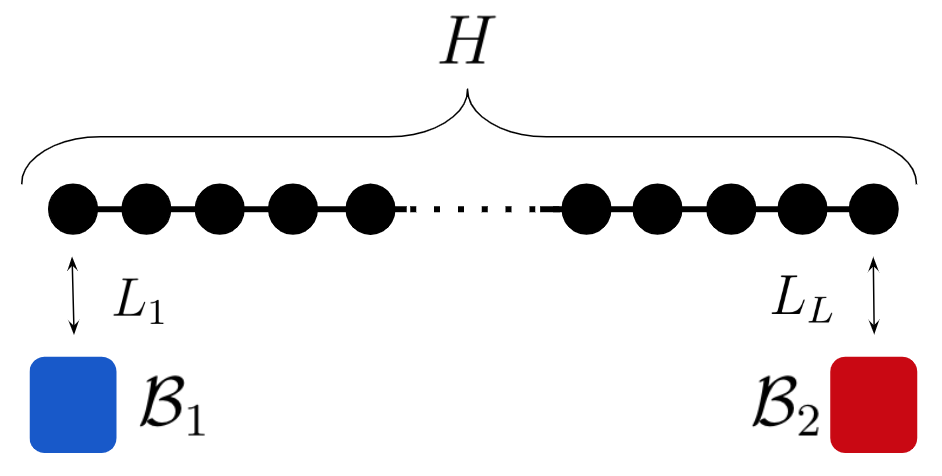
\includegraphics[scale=0.7]{Figures/sketch_model.png}
    \captionsetup{width=1.\linewidth}
    \caption{Sketch of the model under study. The system is described by an Hamiltonian $H$; $\mathcal{B}_1$ and $\mathcal{B}_2$ are the baths coupled to the boundaries of the chain by the Lindblad operators $L_1$ and $L_L$. In this thesis, $\mathcal{B}_1$ ($\mathcal{B}_2$) is the bath that ``pumps'' spin up (down), but another similar system could be coupled to two reservoirs with two different temperatures. In that case, one could study a temperature gradient, instead of magnetization and spin current.}
    \label{fig:sketch_model}
\end{figure}

%B_1(blue) è il bagno che pompa gli spin up, B_2(red) gli spin down; uno può descrivere questo sistema come l'azione ai bordi accoppiati a due bagni (uno l'opposto dell'altro) usando un linguaggio di spin. Un'altra scelta (non fatta nella tesi) potrebbe essere quella di prendere due bagni a diverse temperature: hot and cold reservoir e si genera un gradiente di temperatura. In questa tesi si studia cosa succede alla magnetizzazione quando si dà un bias diverso a sinistra e a destra, ma nulla vieta di prendere due temperature diverse e si va a studiare il gradiente termico o corrente termica/energia.

The physics of this model represents in a realistic way some behaviours of the Hubbard models described in chapter~\ref{chapter2}, i.e. the models tipically studied by quantum simulators.

In the following sections, we will study three fundamental observables: the magnetization profile, the two-point correlation function, the spin current; in particular, we will examine them in chains of different size: 8, 12, 16 sites. 

All fits in the present and in the next chapters are made with Minuit/Migrad and Linear minimizers~\cite{root_cern}.

%%%%%%%%%%%%%%%%%%%%%%%%%%%%%%%%%%%%%%%%%%%%%%%%%%%%%%%%%%%%%%%%%%
%%%%%%%%%%%%%%%%%%%%%%%%%%%%%%%%%%%%%%%%%%%%%%%%%%%%%%%%%%%%%%%%%%
%%%%%%%%%%%%%%%%%%%%%%%%%%%%%%%%%%%%%%%%%%%%%%%%%%%%%%%%%%%%%%%%%%
\section{Magnetization Profile}
\label{sec:magn_profile}
The first observable we want to examine is the magnetization profile of the chain, i.e. the expectation value $\langle \sigma_i^z \rangle$ of the Pauli matrix $\sigma^z$ for each site:
\begin{equation*}
    \langle \sigma_i^z \rangle = \Tr(\sigma_i^z \rho_s),
\end{equation*}
being $\rho_s$ the steady-state density matrix of the system.

The magnetization profile is the first marker of the dynamics of the chain:  it reveals the responsivity of the system to the competing polarizing effects of the two baths; in particular, it allows us to see the effects generated by the presence of the dissipators, described by the Lindblad operators~\ref{dissipators}. One should expect the profile to have the ends polarized toward opposite directions, because of the position (in the first and in the last chain site) of the dissipators.

The behaviour of magnetization along z spin direction is shown in fig.~\ref{fig:LM_comparisonVSsizeJz1Gamma1}; it is congruent with the reasoning made before. The profile is antisymmetric in respect to the center of the chain, while the first half is characterized by positive values of  $\langle \sigma_i^z \rangle$ and the second half by negative values of $\langle \sigma_i^z \rangle$, because the first dissipator (positioned in the first site) forces spins to align along the positive z-axis. The opposite happens for the second dissipator.

%Moreover, in order to make sure the numerical results are under control, a comparison between MPO and QT methods is done for a 8-sites chain. It is clear that the results are overlapping, so it is reasonable to treat them as plausible ones.

%\begin{figure}[H]
    %\centering
    %\includegraphics[scale=0.7]{Figures/8sites/LMComparison_8sJ105%1.pdf}
    %\captionsetup{width=1.\linewidth}
    %\caption{Spin profile for a 8-sites chain characterized by %$\gamma=1, J_x=1, J_y=1, J_z=1$; \\ \emph{i} stands for the %site index.}
    %\label{fig:8sites_LMcomparisonJz1}
%\end{figure}

Now, it is interesting to investigate how the size of the chain influences the magnetization profile. Fig.~\ref{fig:LM_comparisonVSsizeJz1Gamma1} displays a comparison between the magnetization profile of chains with different lengths. In order to do so, we have scaled the x-axis so that the ends are 0 and 1. Two characteristics stand out: the first one is the fact that the peak values of $\langle\sigma_i^z\rangle$ in the ends of the chain are independent of the size of the system; this is true also for different values of $\gamma$: the peak values still remain the same for different lengths of the chain; the second one involves the fact that increasing the length of the chain, the spin profile gets flatter.

\begin{figure}[H]
    \centering
    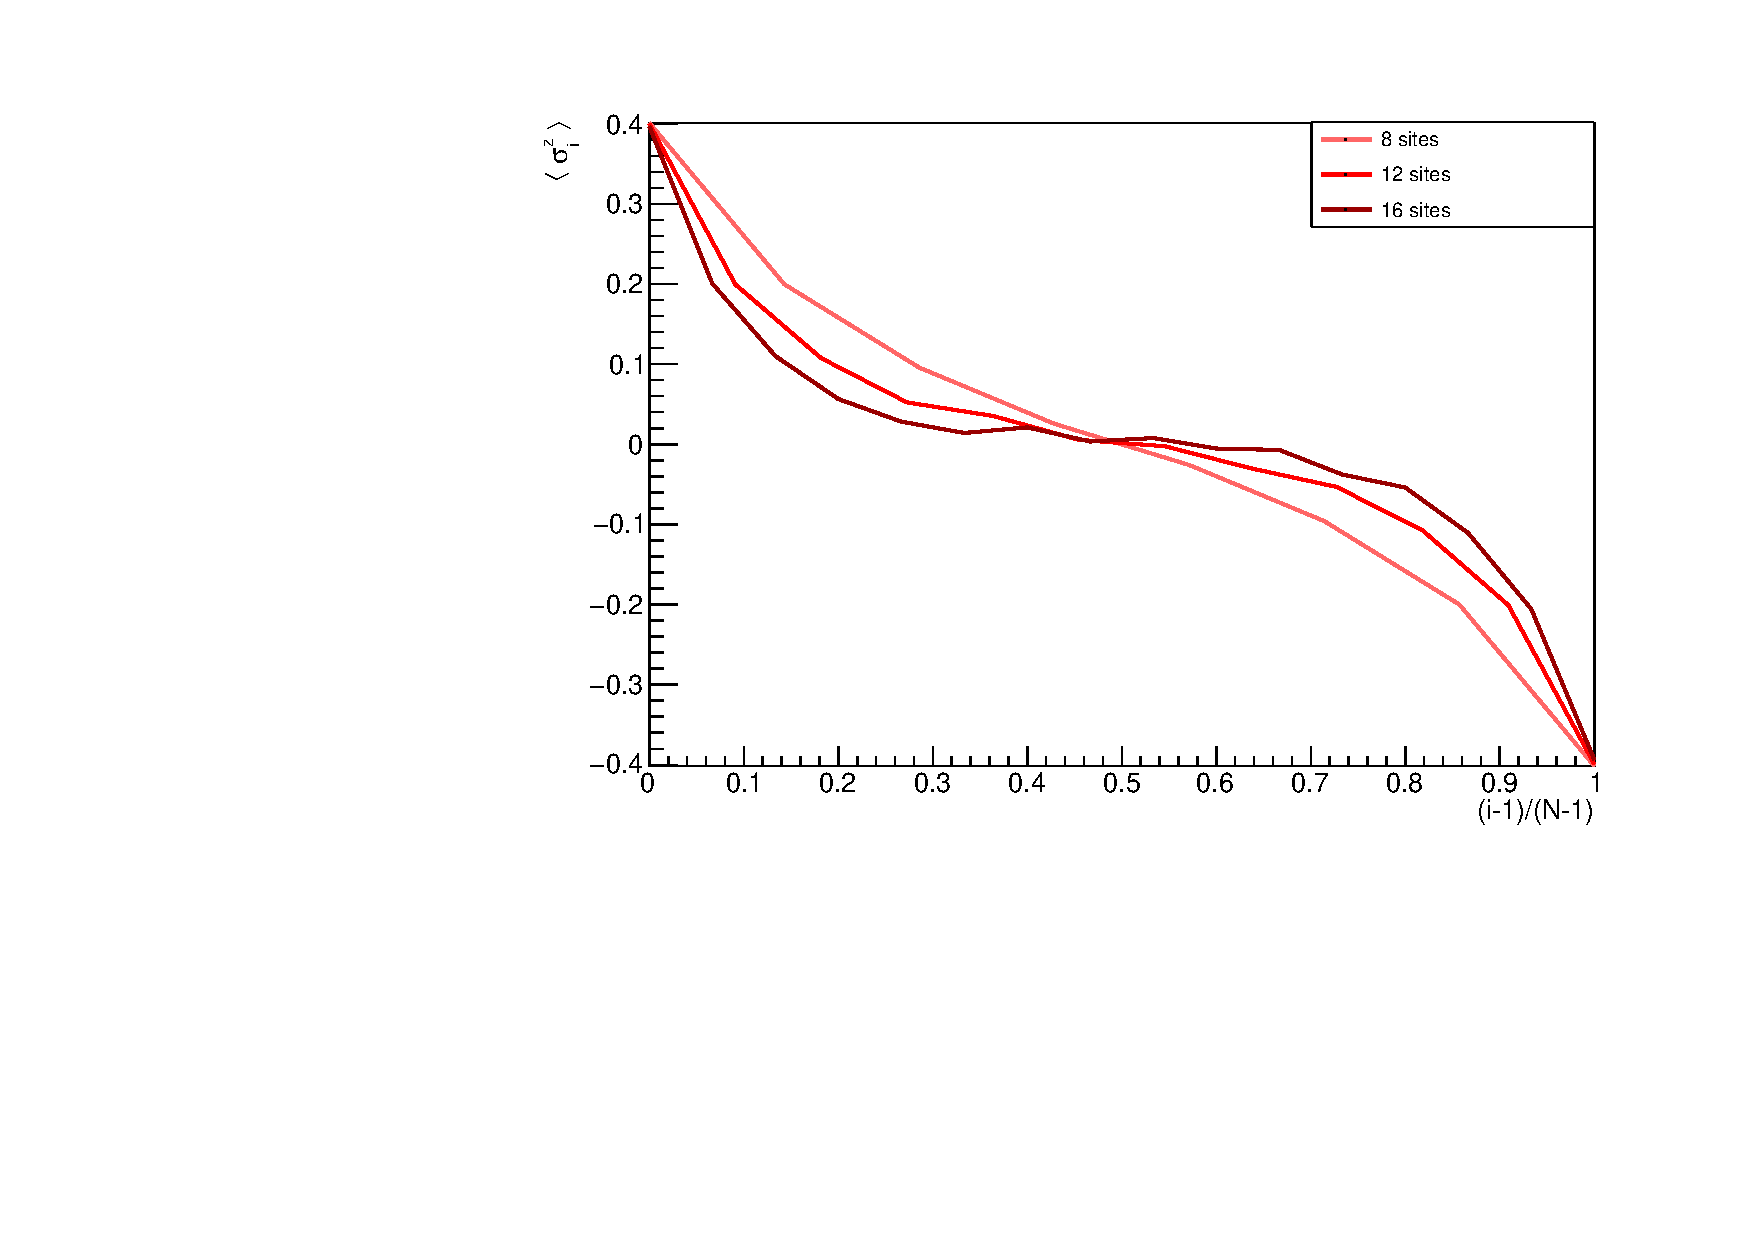
\includegraphics[scale=0.7]{Figures/NORM_LM_comparisonVSsize.pdf}
    \captionsetup{width=1.\linewidth}
    \caption{Spin magnetization profile along the z axis as a function of the position inside the chain, rescaled between 0 and 1, at $J_z = 1$ and $\gamma=1$. Data for different chain lengths are shown and they are obtained from MPO method.}
    \label{fig:LM_comparisonVSsizeJz1Gamma1}
\end{figure}

In order to analyze these properties in more detail, in the following figures we see how the behaviour of magnetization profile changes for different values of dissipation rate $\gamma$. 

First of all, it is convenient to separate the curves for each size (8, 12 and 16 sites) in order to distinguish the profiles. The plots are shown in figures~\ref{fig:LMvsGamma3panelsSizes}.

Several aspects of our numerical outcomes are worth to be noted and commented. First of all, it seems clear that, while increasing $\gamma$, the ends of the chain become more and more polarized. This is true for every length of the chain because, as mentioned previously, the peak values are independent of the length of the chain.

The profile for the 8-sites chain (upper panel in fig.~\ref{fig:LMvsGamma3panelsSizes}) seems to be almost linear, but this is due to size effect: indeed, for 12 and 16-sites chain (middle and bottom panels of fig.~\ref{fig:LMvsGamma3panelsSizes}) the non-linear trend becomes more and more evident as the length increases. Indeed, while $L$ grows, the plots show with increasing clarity the formation of a \emph{plateau} in the bulk of the system, in which the magnetization is zero; only near the edges the profile tends to deviate from the plateau, because of the driving effect of the dissipators.
%Only near the edges it tends to differ from zero, because of the driving effect of the dissipators. 

\begin{figure}[H]
\centering
%\begin{subfigure}{\columnwidth}
%\centering
    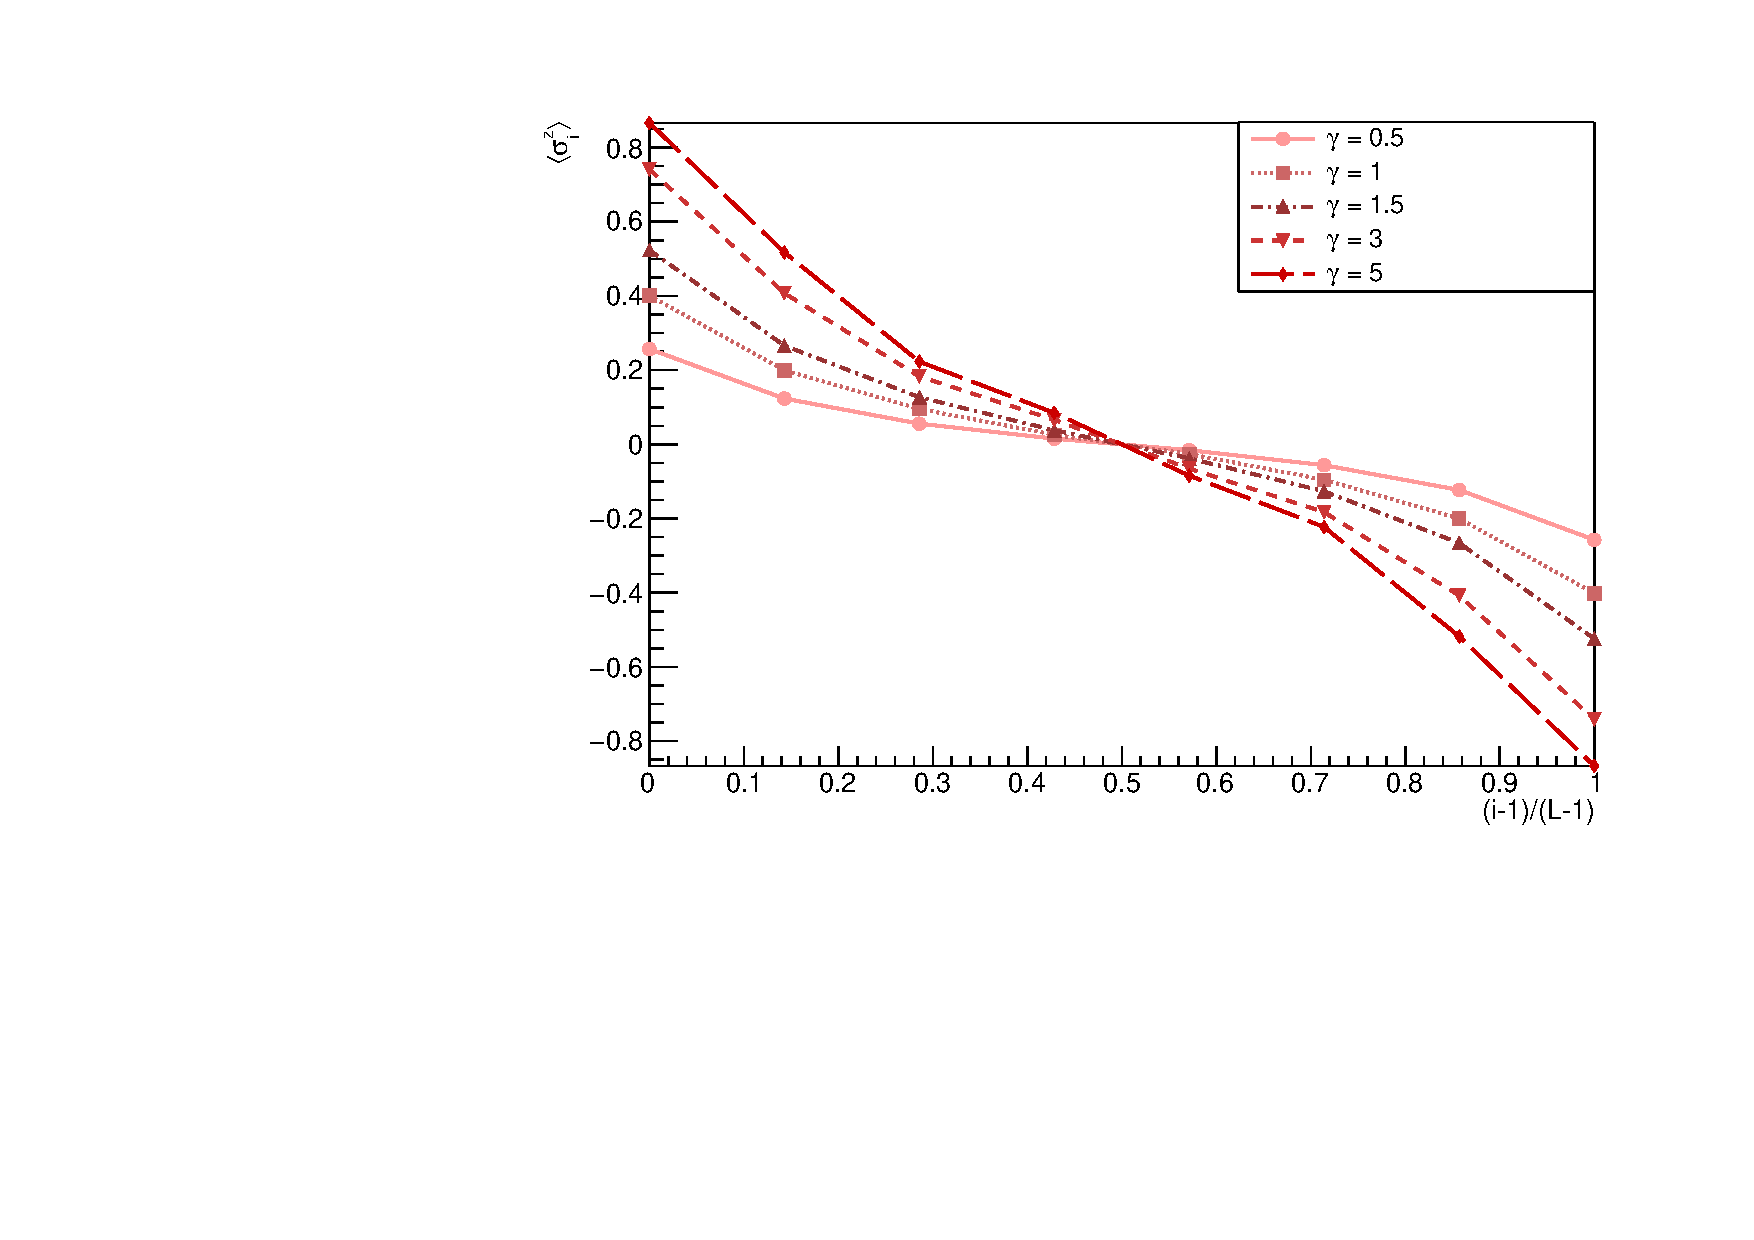
\includegraphics[scale=0.55]{Figures/8sites/8sites_LMvsGamma.pdf}
    \label{fig:8sites_LMvsGamma}
%\end{subfigure}
%\begin{subfigure}{\columnwidth}
%\centering
    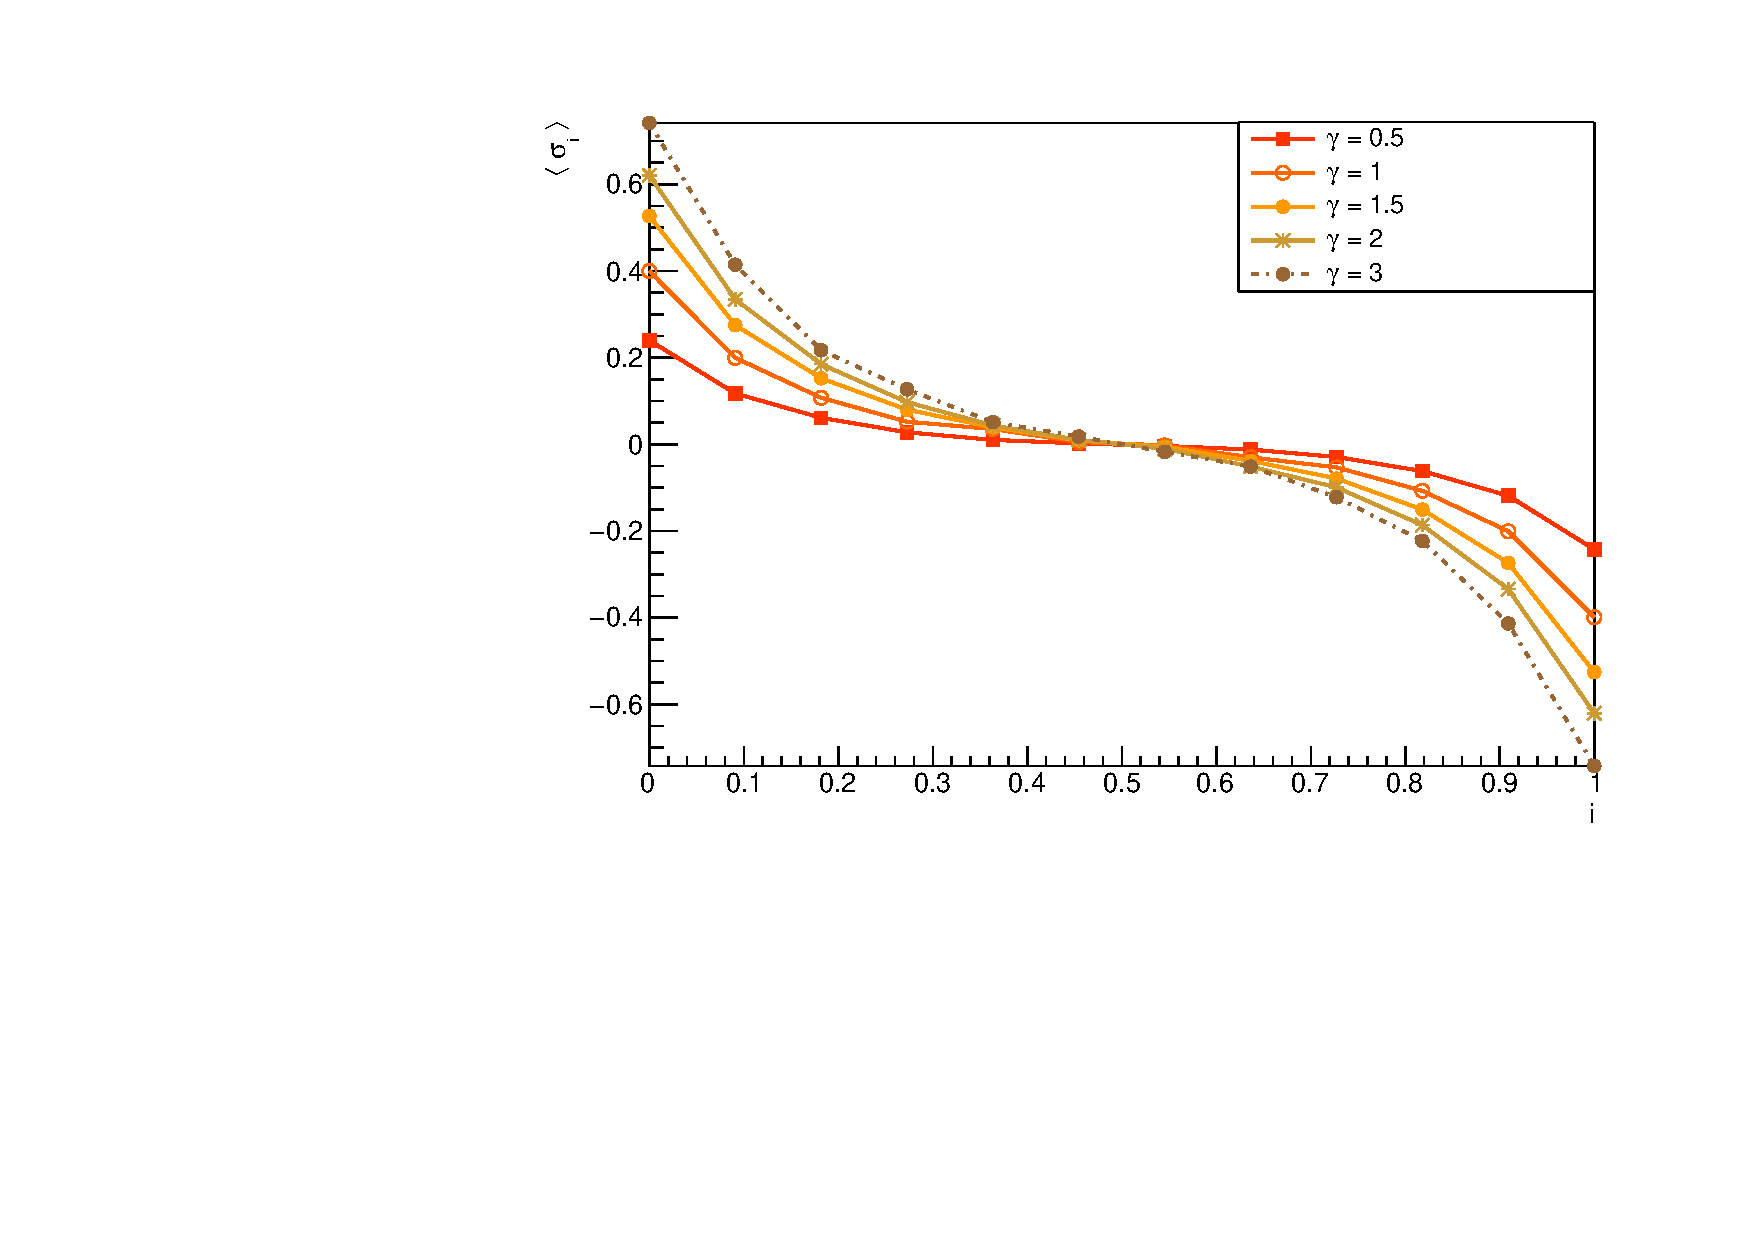
\includegraphics[scale=0.55]{Figures/12sites/12sites_LMvsGamma.pdf}
    \label{fig:12sites_LMvsGamma}
%\end{subfigure}
%\begin{subfigure}{\columnwidth}
%\centering
    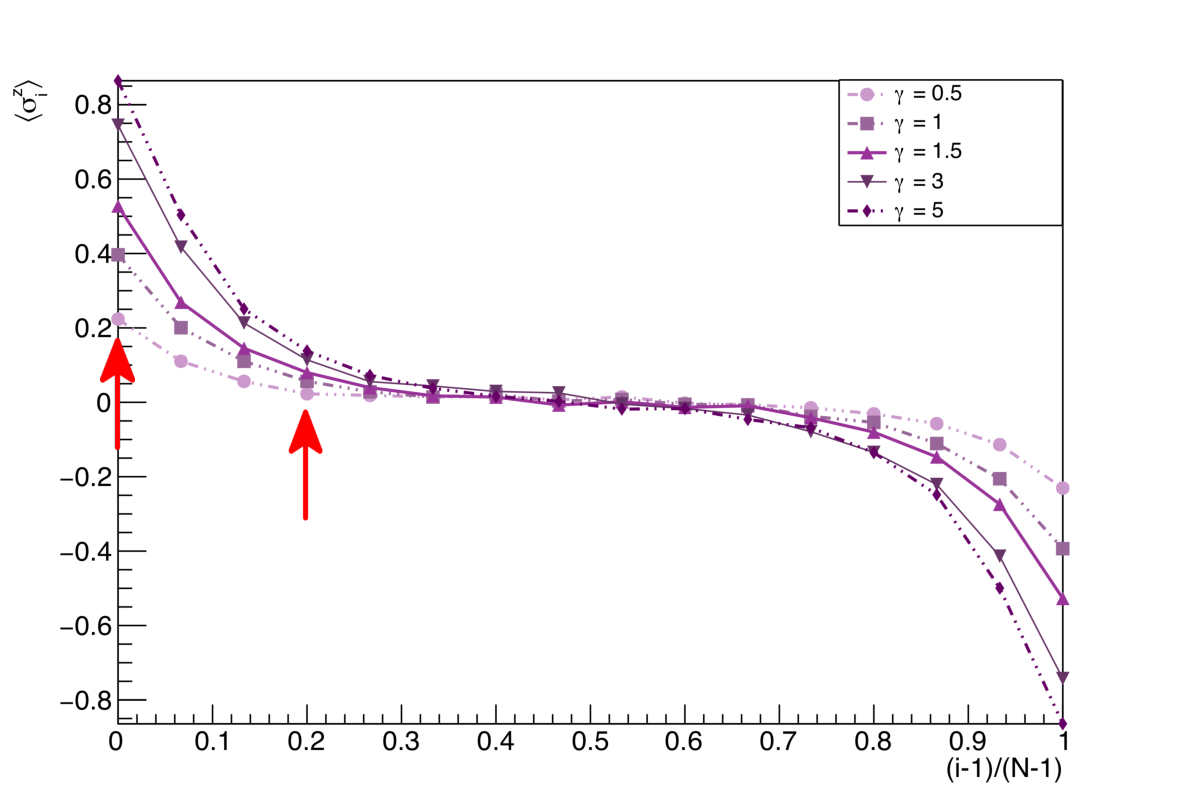
\includegraphics[scale=0.55]{Figures/16sites/16sites_LMvsGamma.pdf}
    \label{fig:16sites_LMvsGamma}
%\end{subfigure}
\captionsetup{width=1.\linewidth}
\caption{Spin profile for a 8-sites chain (upper panel), 12-sites chain (central panel), 16-sites chain (bottom panel) varying on dissipation rate $\gamma$. Data are obtained from MPO method. The red arrows point at two sets of values that will be analyzed in the following.}
\label{fig:LMvsGamma3panelsSizes}
\end{figure}

As said previously, the peak value of $\langle\sigma^z\rangle$ varies with $\gamma$. In the upper panel in fig.~\ref{fig:LM_PeakAnd4th_vsGamma} we present the fit~\cite{root_cern} that shows an exponential behaviour. It is interesting to note that the same dependence is also kept also by $\langle\sigma^z\rangle$ of spins lying in the $\frac{L}{4}$-th site (see the bottom panel in fig.~\ref{fig:LM_PeakAnd4th_vsGamma}); the same trend is confirmed in the case of 8 and 12 sites.

The dependence shown by the fit is the following:
\begin{equation*}
    \langle \sigma^z \rangle(\gamma) = p_0 (1- e^{-p_1\gamma}).
\end{equation*}
In fig.~\ref{fig:LM_PeakAnd4th_vsGamma} the fit parameters for each plot are shown.

\begin{figure}[H]
\centering
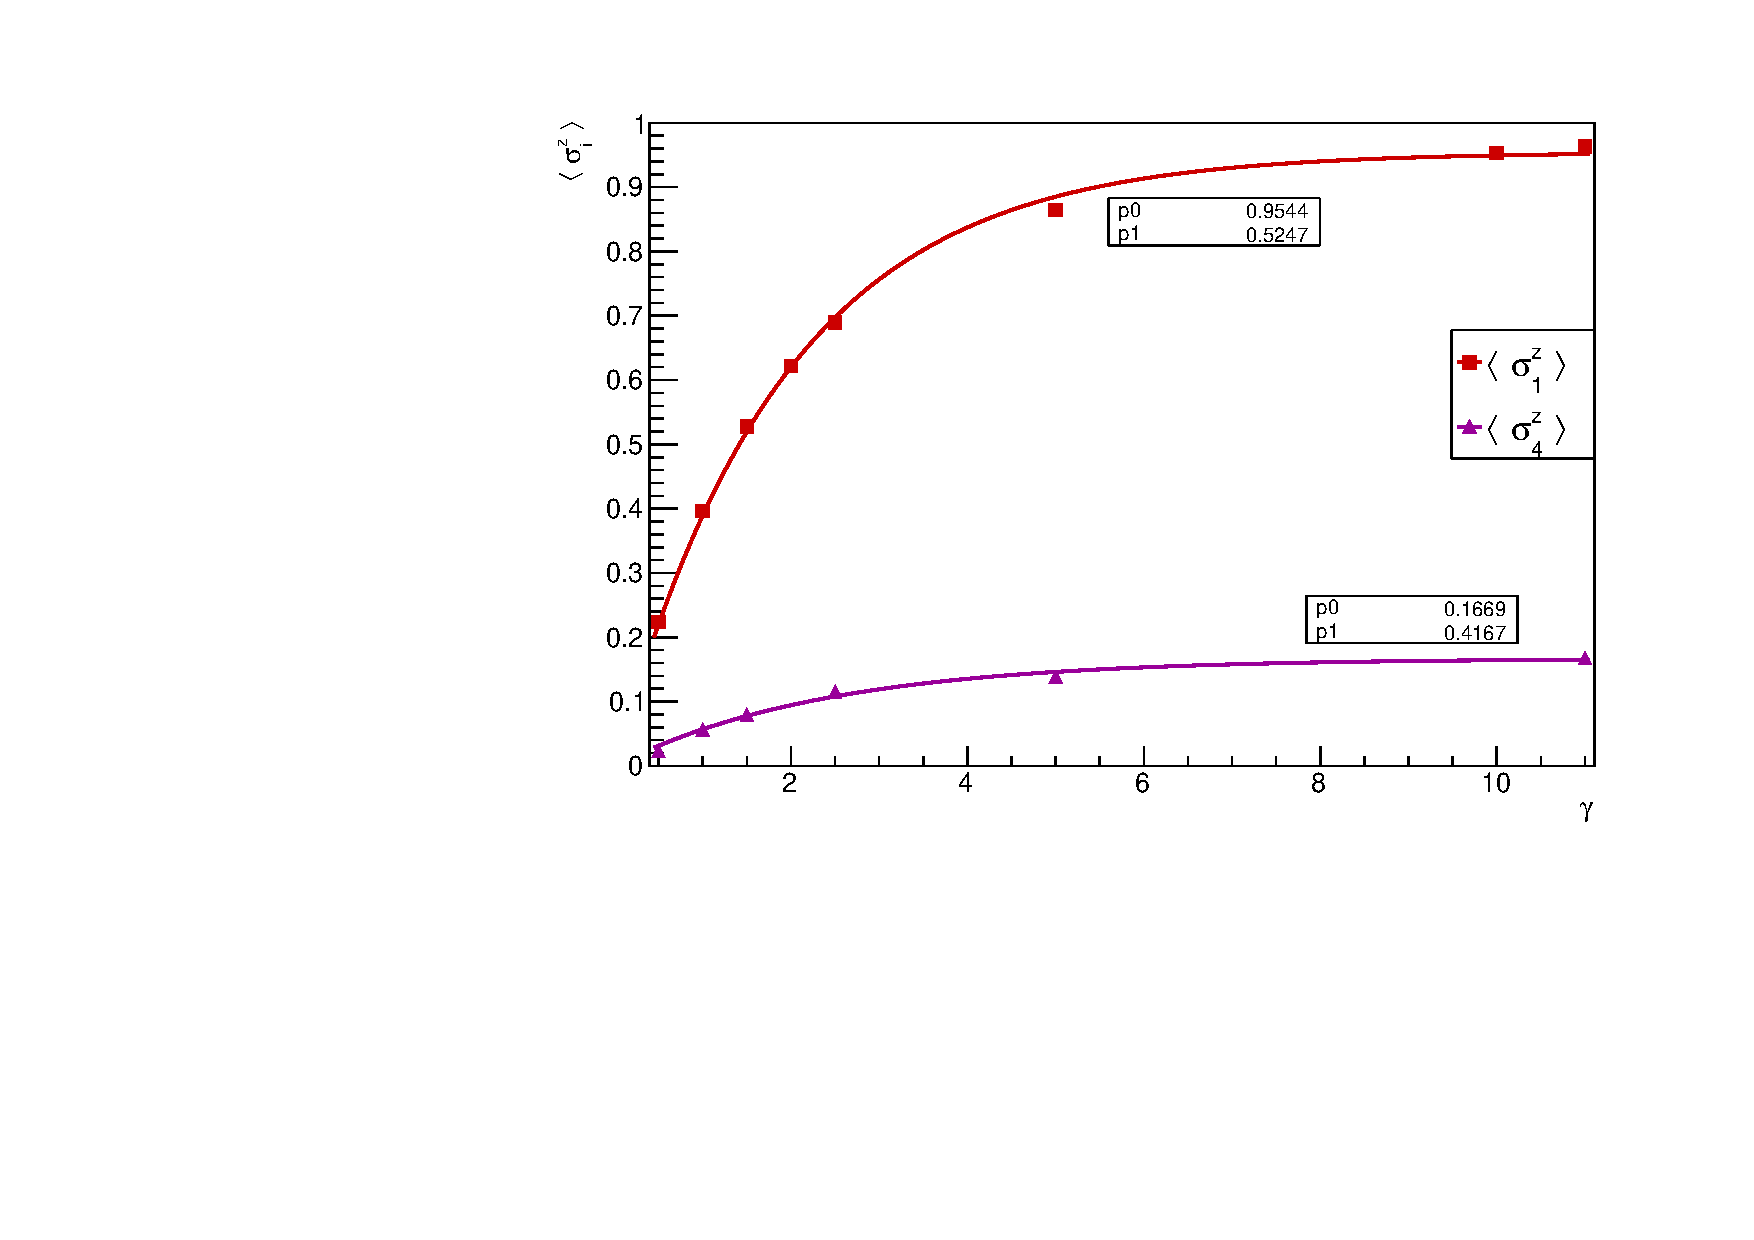
\includegraphics[scale = 0.6]{Figures/LMvsGammaVsSiteIndex.pdf}
\captionsetup{width=1.\linewidth}
\caption{In red, the fit of the magnetization of the first site of the chain (coupled to the dissipator described by $\sigma^+$); in purple, the fit of the magnetization of the forth spin of the chain of 16 sites.}
\label{fig:LM_PeakAnd4th_vsGamma}
\end{figure}

These two plots displayed in fig.~\ref{fig:LM_PeakAnd4th_vsGamma} show that for large values of $\gamma$, i.e. for more and more important driving, $\langle\sigma^z\rangle$ tends asymptotically to a maximum value.

Studying the gradient of the magnetization $\nabla \langle \sigma^z \rangle$ with respect to the position, we have found that its trend is consistent with the profiles just shown.

%In the following, we study the gradient of magnetization for the middle sites in the 8-sites chain. In fig.~\ref{fig:FIT_8sites_gradLM23VSgamma}, \ref{fig:FIT_12sites_gradLM34VSgamma}, \ref{fig:FIT_16sites_gradLM45VSgamma} the gradient of magnetization between the spin lying in the $\frac{N}{4}$-th site and the neighbouring site. The profile here shown, seems to confirm the fits in fig.\ref{fig:FIT8sites_LM_2ndSiteVSgamma}, \ref{fig:FIT12sites_3rdSiteVSgamma}, \ref{fig:FIT_16sites_4thSiteVSgamma}.

%\begin{figure}[H]
    %\centering
    %\includegraphics[scale=0.7]{Figures/8sites/FIT_8sites_gradLMcente%rVSgamma.pdf}
    %\caption{8 sites, the red line shows the fit \\$\nabla %\langle\sigma^z\rangle_{center}(\gamma) = %-p_0+p_1\exp{(-p_2\gamma)}$.}
    %\label{fig:FIT_8sites_gradLMcenterVSgamma}
%\end{figure}

%\begin{figure}[H]
    %\centering
    %\includegraphics[scale=0.7]{Figures/8sites/FIT_8sites_gradLM23VSg%amma.pdf}
    %\caption{8 sites, the red line shows the fit \\$\nabla %\langle\sigma^z\rangle_{2-3}(\gamma) = %-p_0+p_1\exp{(-p_2\gamma)}$.}
    %\label{fig:FIT_8sites_gradLM23VSgamma}
%\end{figure}

%\begin{figure}[H]
    %\centering
    %\includegraphics[scale=0.7]{Figures/12sites/FIT_12sites_gradLM34V%Sgamma.pdf}
    %\caption{12 sites, the orange line shows the fit \\$\nabla %\langle\sigma^z\rangle_{3-4}(\gamma) = %-p_0+p_1\exp{(-p_2\gamma)}$.}
    %\label{fig:FIT_12sites_gradLM34VSgamma}
%\end{figure}

%\begin{figure}[H]
    %\centering
    %\includegraphics[scale=0.7]{Figures/16sites/FIT_16sites_gradLM45V%Sgamma.pdf}
    %\captionsetup{width=1.\linewidth}
    %\caption{16 sites, the black line shows the fit $\nabla %\langle\sigma^z\rangle_{4-5}(\gamma) = %-p_0+p_1\exp{(-p_2\gamma)}$.}
    %\label{fig:FIT_16sites_gradLM45VSgamma}
%\end{figure}

%In the following, a comparison between the profiles of the chain of different size.

%\begin{figure}[H]
    %\centering
    %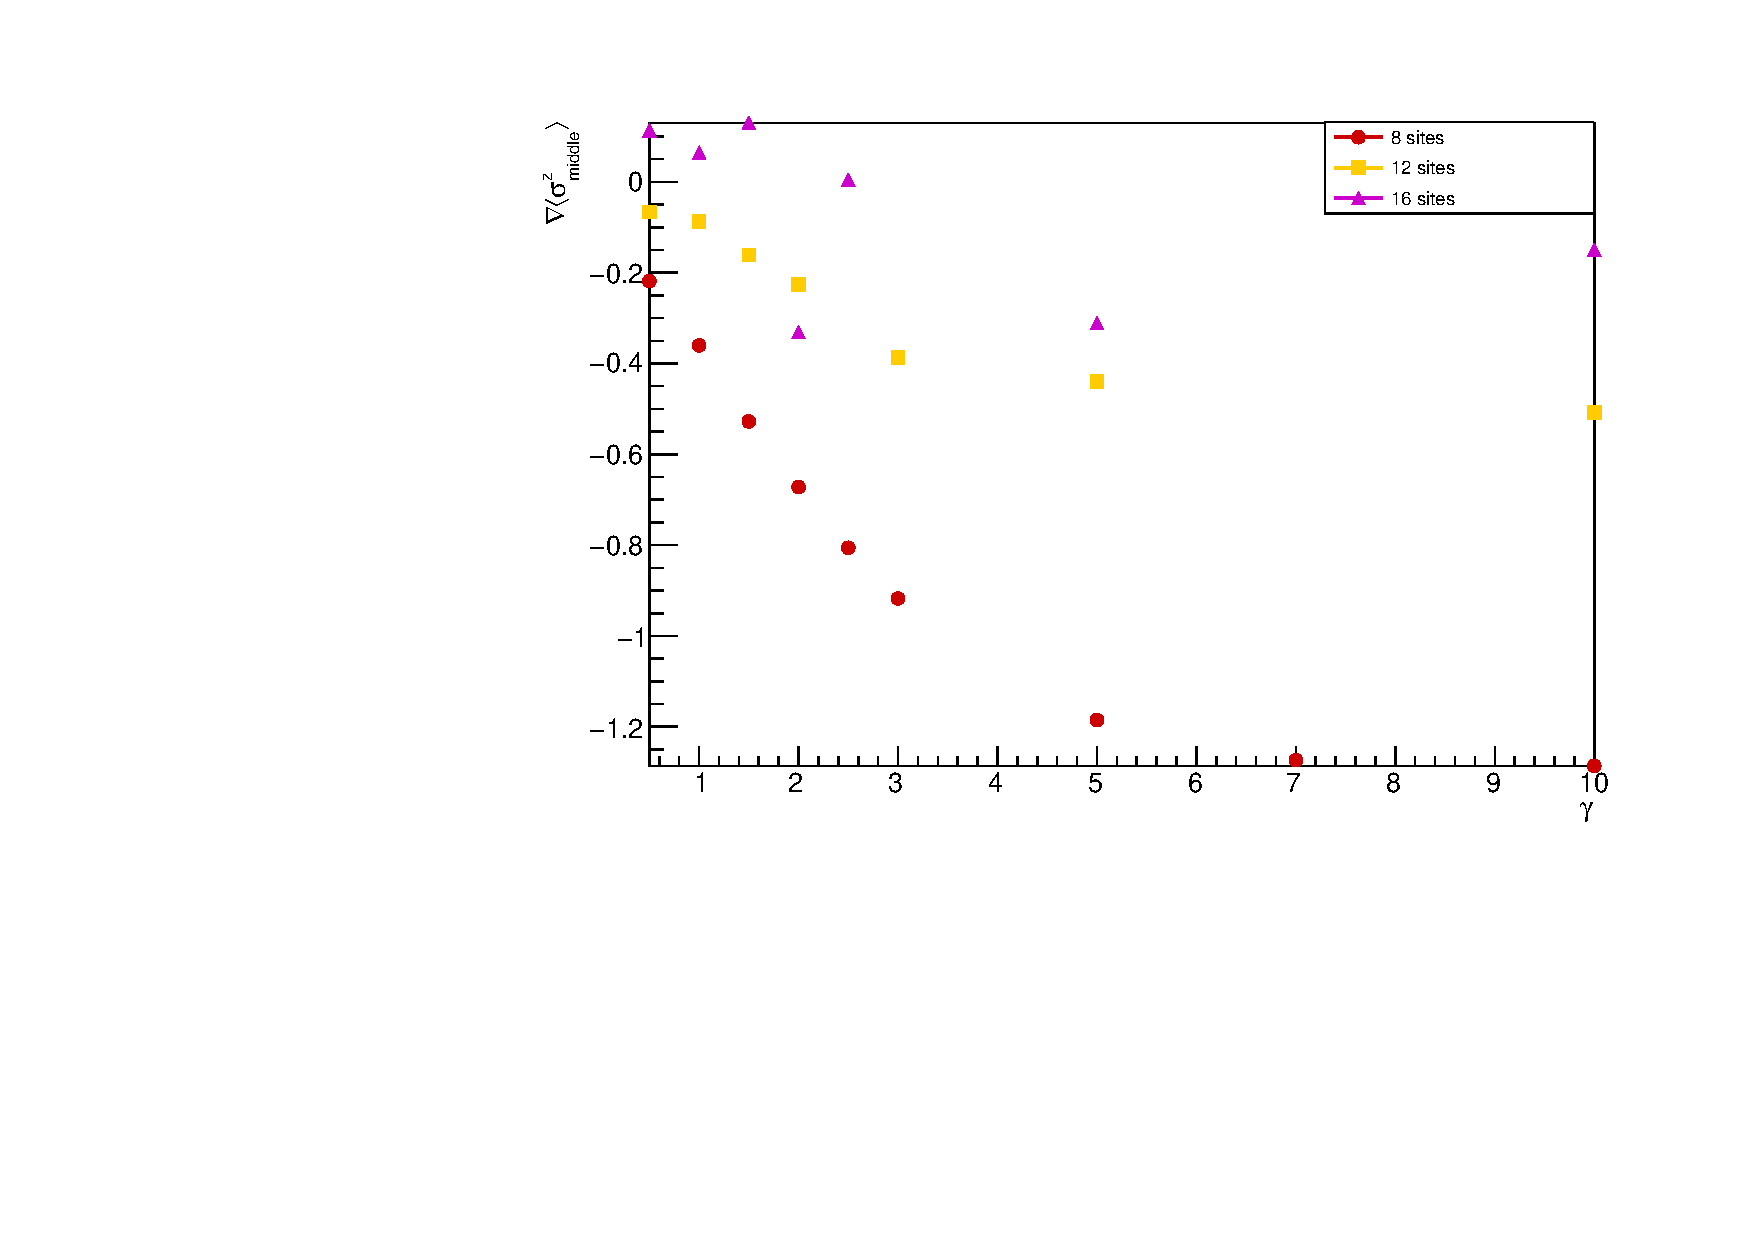
\includegraphics[scale=0.7]{Figures/gradLMvsGammavsSize.pdf}
    %\caption{Gradient of magnetization for the middle sites in 8, 12, %16-sites chain versus $\gamma$.}
    %\label{fig:gradLMvsGammavsSize}
%\end{figure}

%\begin{figure}[H]
    %\centering
    %\includegraphics[scale=0.7]{Figures/gradLMvsGammavsSize_firstQuar%terChain.pdf}
    %\caption{Gradient of magnetization for the sites lying in the %$\frac{N}{4}$-th site in 8, 12, 16-sites chain versus $\gamma$.}
    %\label{fig:gradLMvsGammavsSize_firstQuarterChain}
%\end{figure}


%%%%%%%%%%%%%%%%%%%%%%%%%%%%%%%%%%%%%%%%%%%%%%%%%%%%%%%%%%%%%%%%%%%%%%%%%%%%%%%%%%%%%%%%%%%%%%%%%%%%%%%%%%%%%%%%%%%%%%%%%%%%%%%%%%%%%%%%%%%%%%%%%%%%%%%%%%%%%%%%%%%%%%%%%%%%%%%%%%%%%%%%%%%%%%%%%%%%%%%%%%%%%%%%%%%%%%%%%%%%%%%%%%%%%%%%%%%%%%%%%%%%%%%%%%%%%%%%%%%%%
\section{Two-Point Correlation Function}
Another observable of interest is the steady-state two-point correlation function, defined as follows:
\begin{equation}
    C(i, j) = \langle \sigma^z_i \sigma^z_j \rangle - \langle \sigma^z_i \rangle \langle \sigma^z_j \rangle,
\end{equation}
where $\langle \sigma^z_i \sigma^z_j \rangle = \Tr(\sigma^z_i \sigma^z_j \rho_{s})$ and $\langle \sigma^z_i \rangle = \Tr(\sigma^z_i \rho_{s})$, being $\rho_{s}$ the steady-state density matrix.

In particular, the two-point correlation function will be studied considering the system symmetry, using the so-called \emph{bulk} correlation function; that is, starting from the middle sites of the chain, the correlation function will be calculated between equidistant sites from the center of the chain. In summary:
\begin{equation*}
    \text{for even} \quad i-j \quad
\end{equation*}

In fig.~\ref{fig:BulkCFvsGamma3panelsSizes} the bulk correlation function for several values of $\gamma$ is shown, for 8, 12 and 16 sites spin chain respectively. An interesting aspect that is quite clear in these plots, involves the finite-size effect; while the size of the chain grows, the exponential profile of the correlation function become more clear. Indeed, only starting from size of 12 sites the exponential profile starts to appear clearly.

\begin{figure}[H]
\centering
\begin{subfigure}{\columnwidth}
\centering
    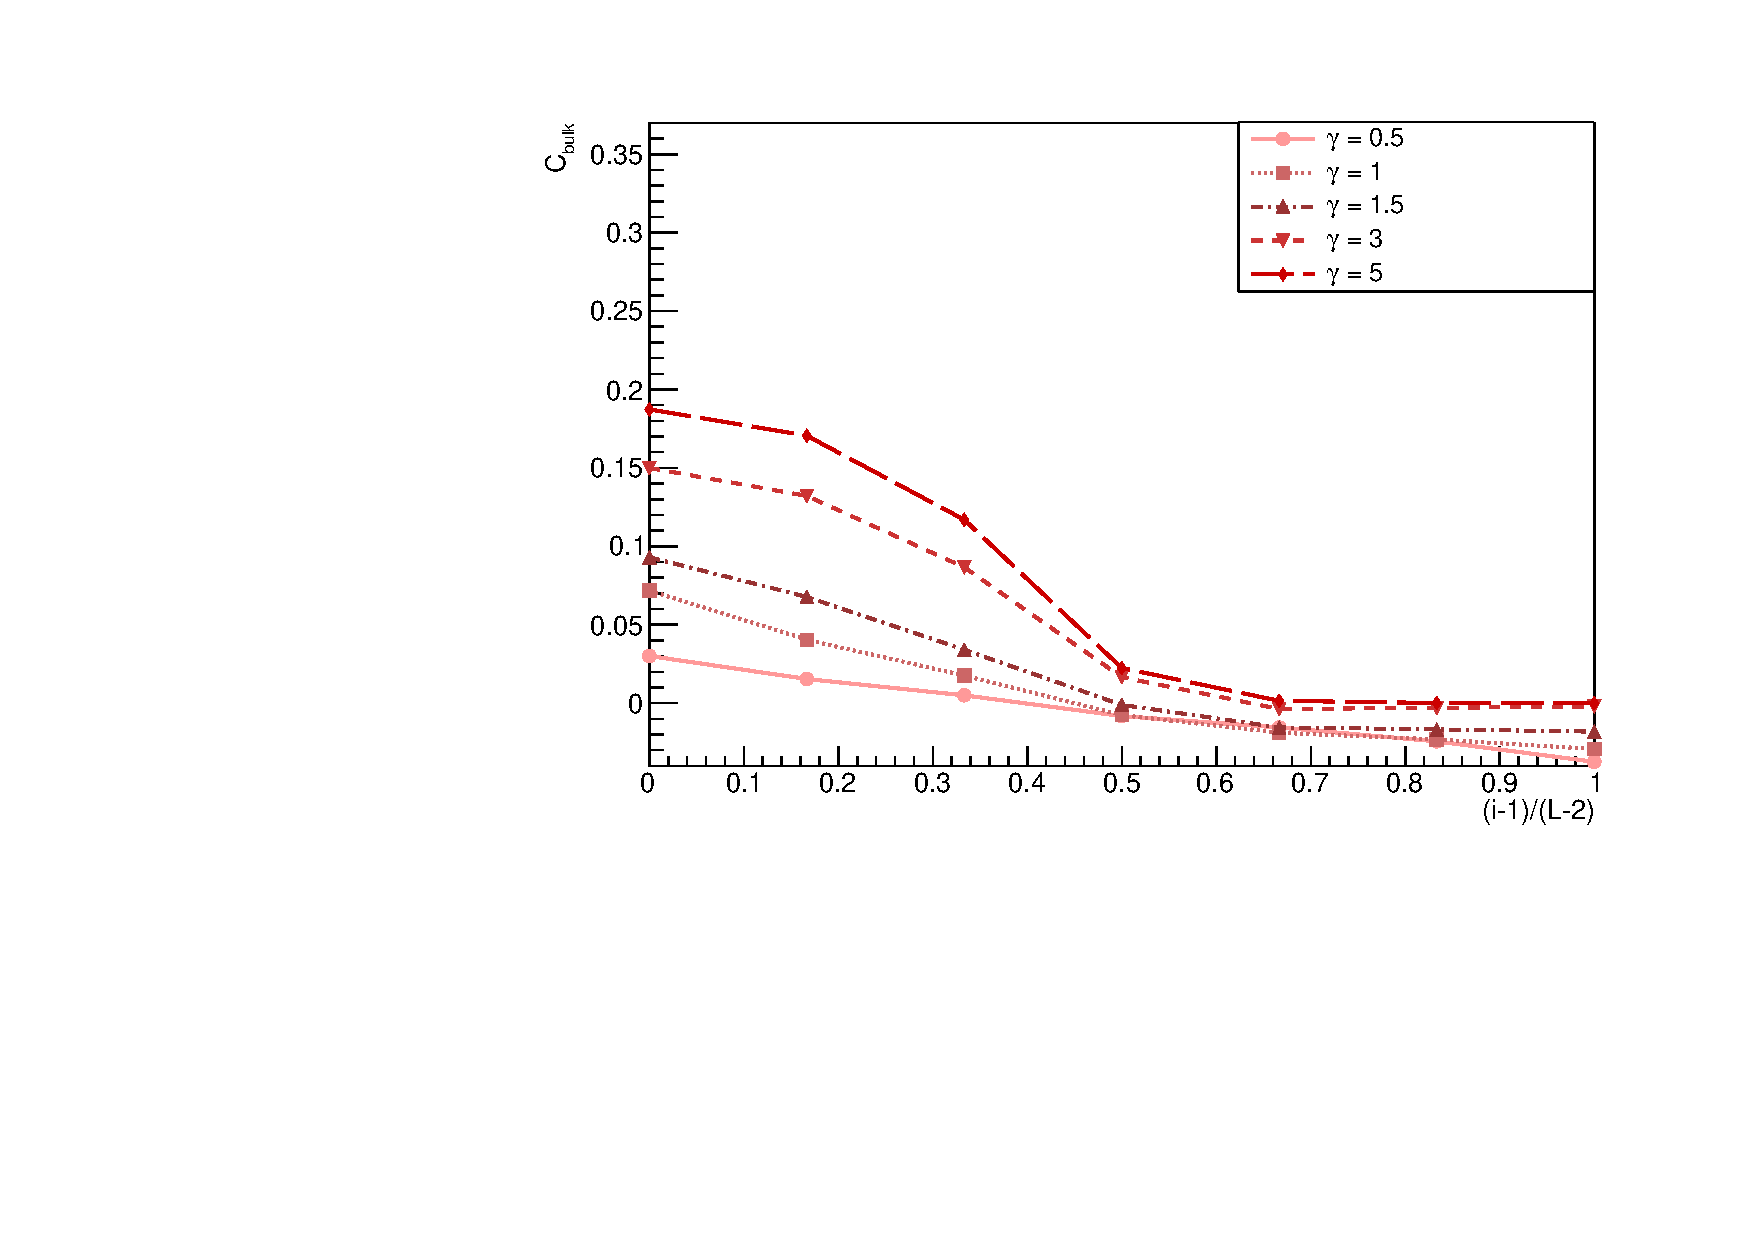
\includegraphics[scale=0.55]{Figures/8sites/8sites_BulkCF_CONNvsGamma.pdf}
    \label{fig:8sites_LMvsGamma}
\end{subfigure}\\
\begin{subfigure}{\columnwidth}
\centering
    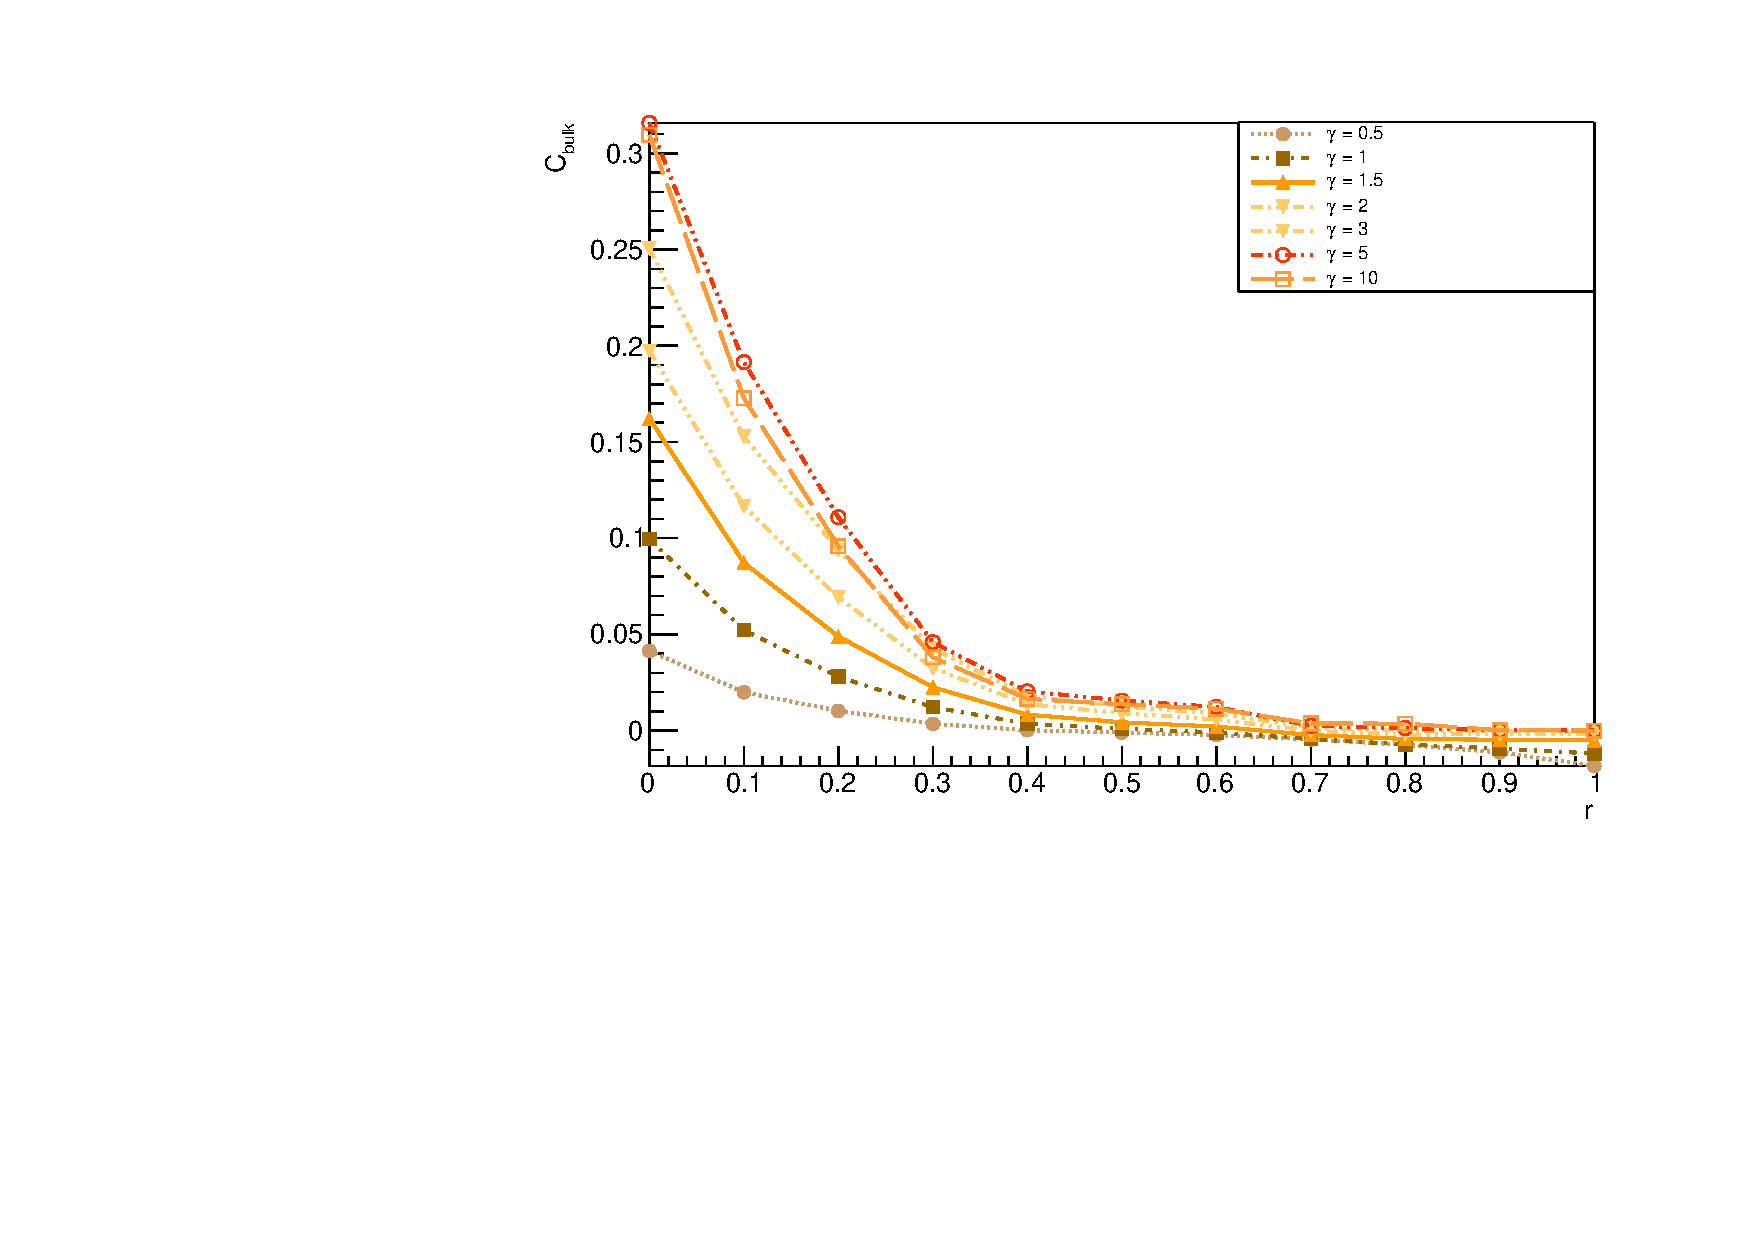
\includegraphics[scale=0.55]{Figures/12sites/12sites_CFBulkCONNVSgamma.pdf}
    \label{fig:12sites_LMvsGamma}
\end{subfigure}\\
\begin{subfigure}{\columnwidth}
\centering
    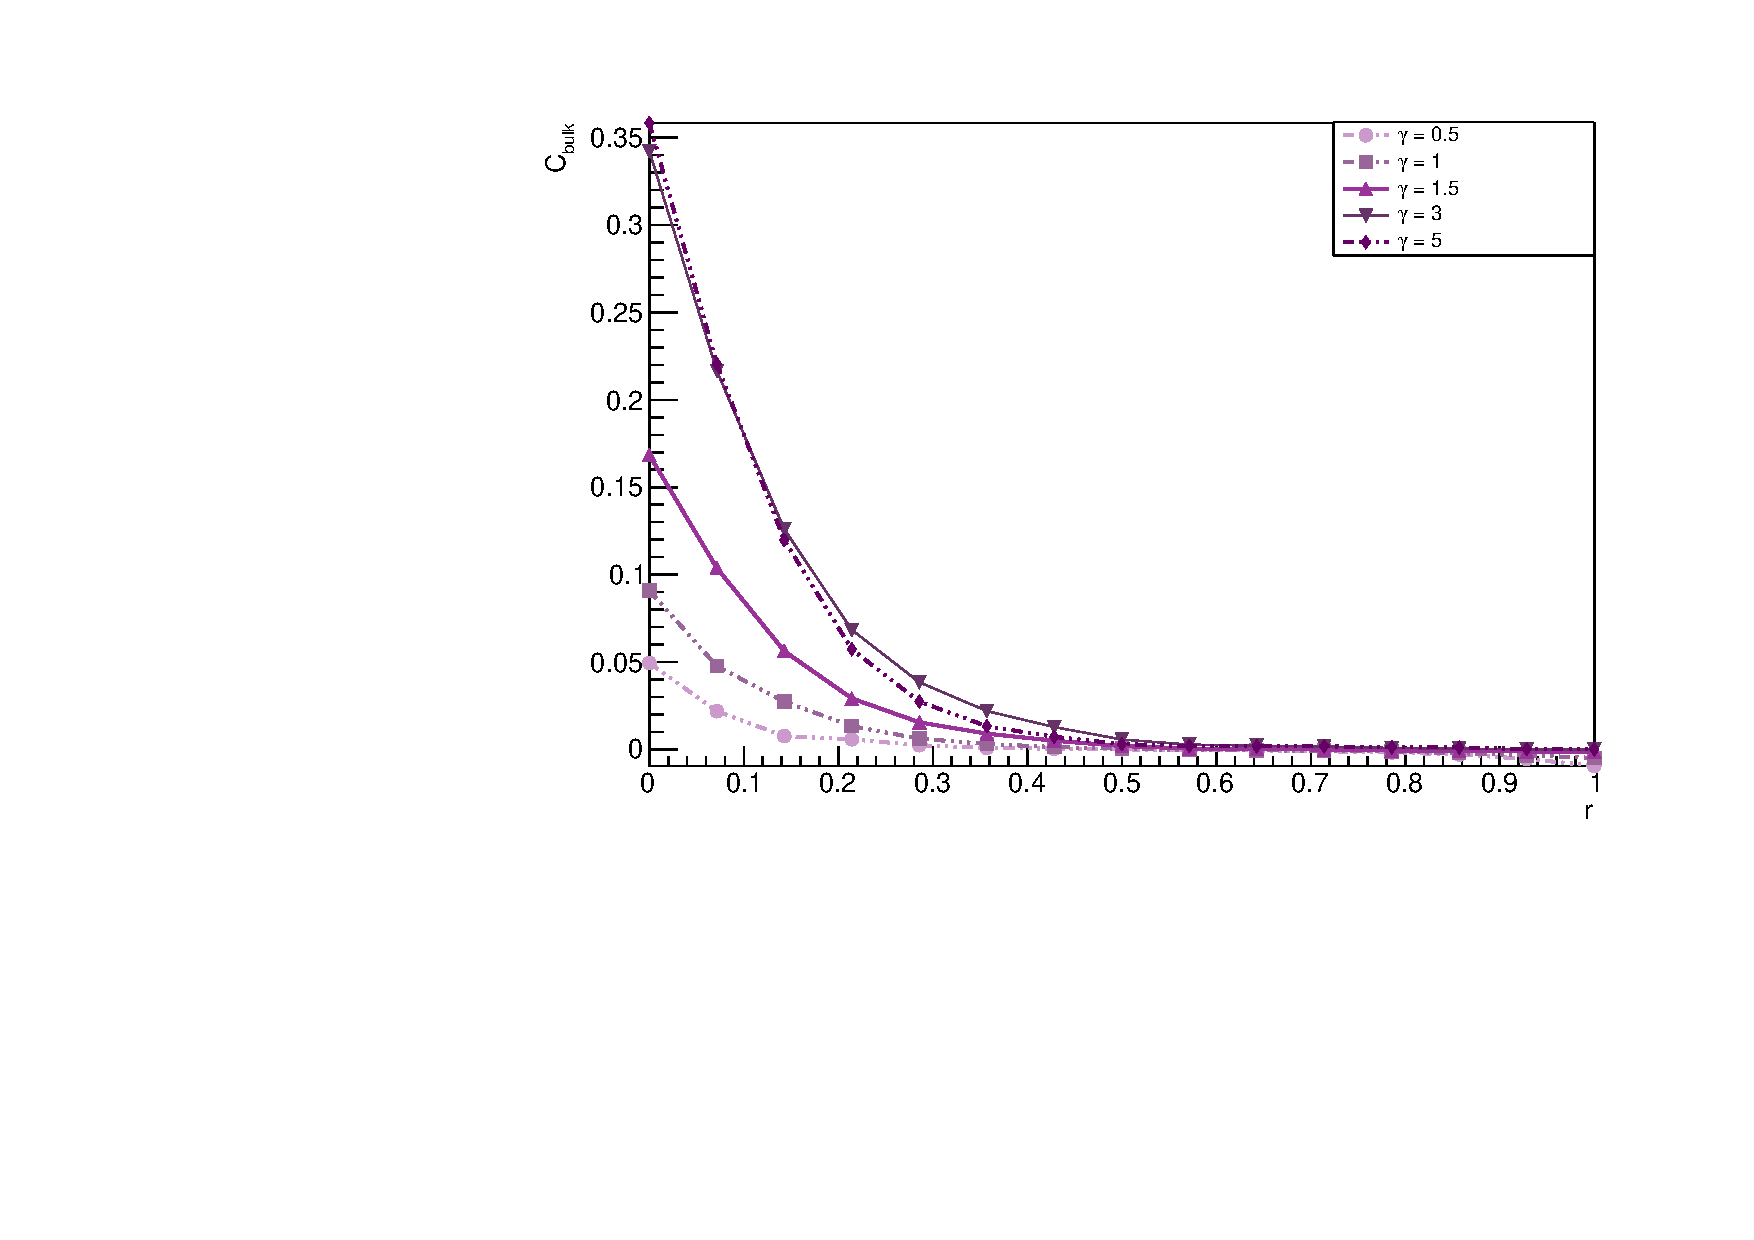
\includegraphics[scale=0.55]{Figures/16sites/16sites_CFBulkCONNVSgamma.pdf}
    \label{fig:16sites_LMvsGamma}
\end{subfigure}\\
\captionsetup{width=1.\linewidth}
\caption{Bulk correlation function for a 8-sites chain (upper panel), 12-sites chain (central panel), 16-sites chain (bottom panel) varying on dissipation rate $\gamma$. Data are obtained from MPO method.}
\label{fig:BulkCFvsGamma3panelsSizes}
\end{figure}

The fit shows that the profile of correlation function is exponential. In fig.~\ref{fig:16sites_FIT_CFBulkCONNvsGamma} several observations can be made; first of all, the trend of the two-point correlation function is exponential. In particular, the dependence from the distance between the spin reads:
\begin{equation*}
    C(r) = p_0 e^{-p_1 r},
\end{equation*}
where the coefficients $p_0$ and $p_1$ are given by the fit and are displayed in fig.~\ref{fig:16sites_FIT_CFBulkCONNvsGamma}. Here, we can see that the correlation between nearest neighbours (i.e. the first point of every curve) gets bigger as $\gamma$ grows.

\begin{figure}[H]
    \centering
    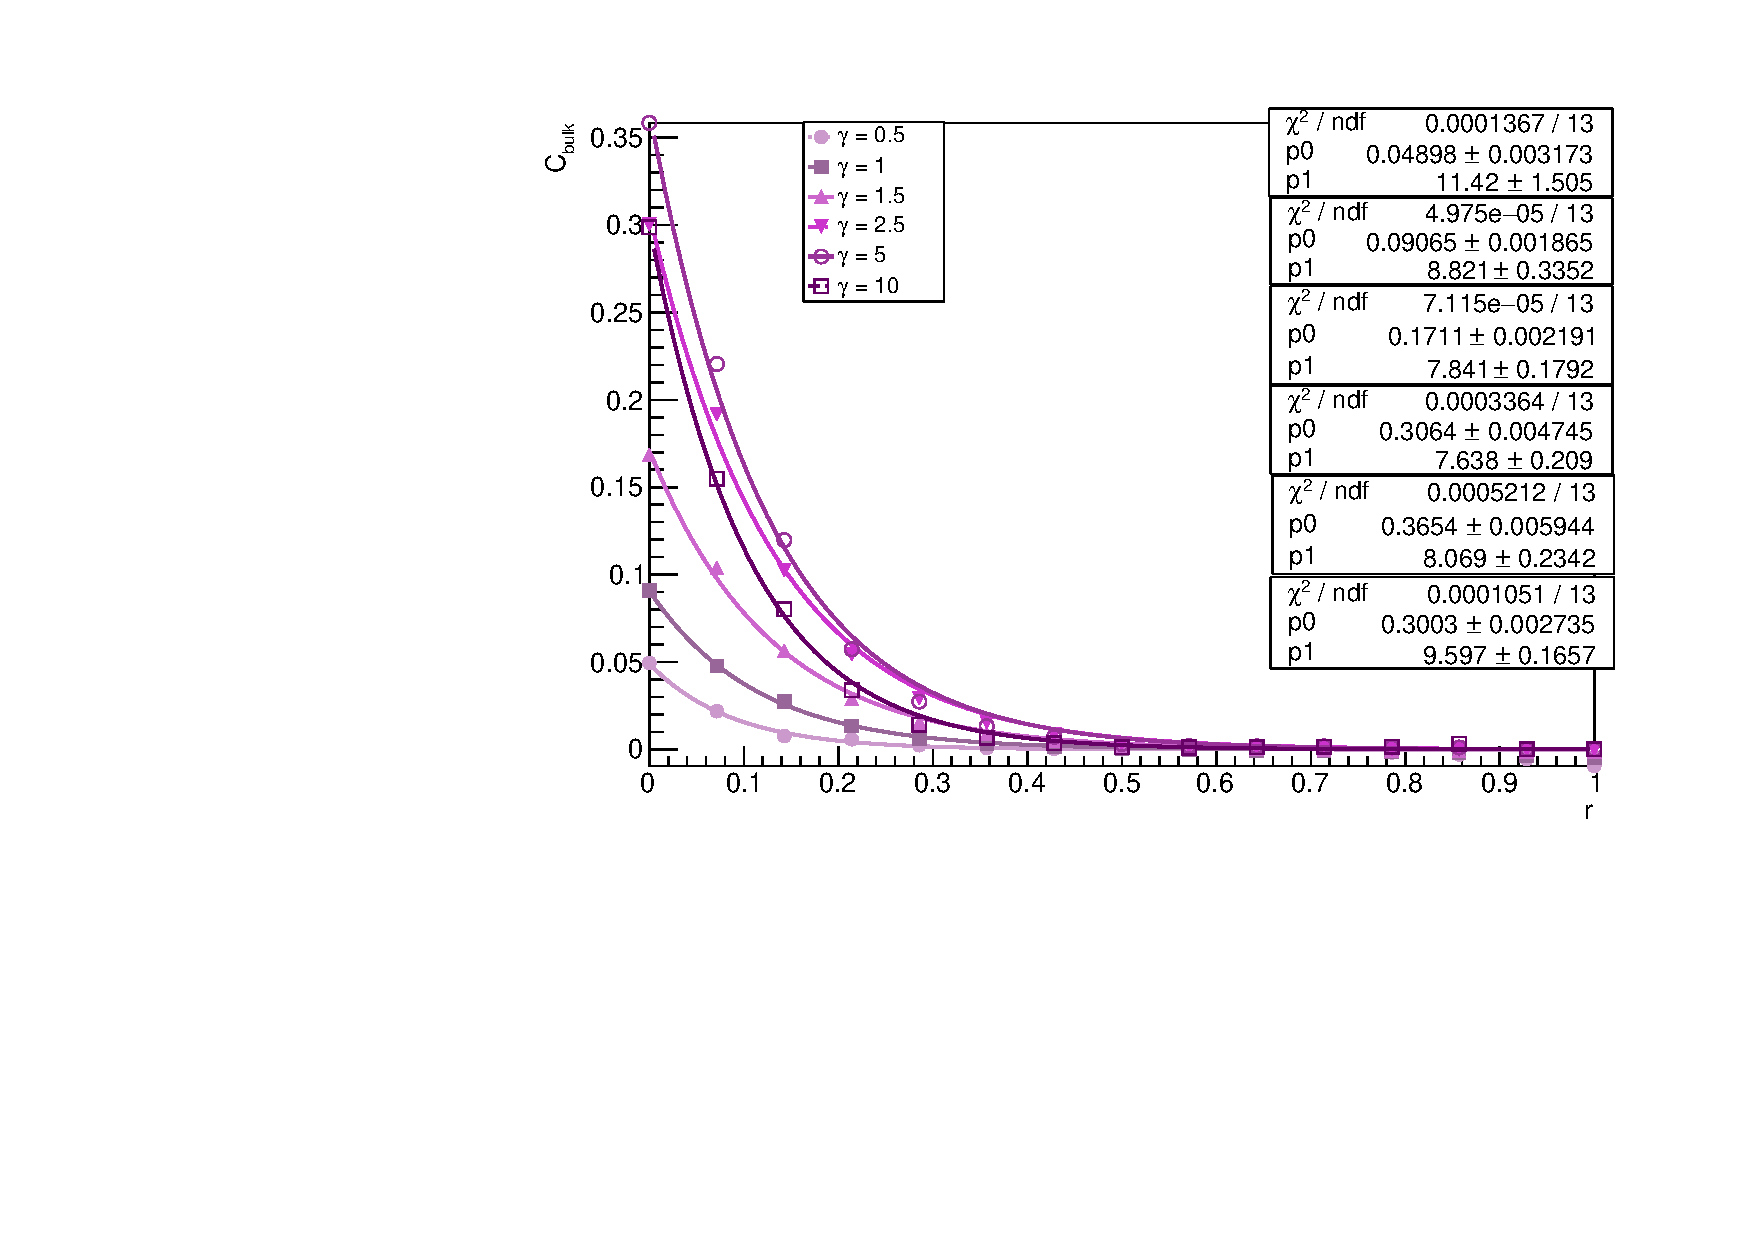
\includegraphics[scale=0.8]{Figures/16sites/FIT_16sites_CFBulkCONN.pdf}
    \captionsetup{width=1.\linewidth}
    \caption{Bulk correlation function for a 16-sites spin chain for several values of $\gamma$. It is shown the fit $C_{\text{bulk}} = p_0 \exp{(-p_1 r)}$. The fit parameters are show in the same order of the legend for $\gamma$. In the box there is the same fit in a semi-logarithmic scale.}
    \label{fig:16sites_FIT_CFBulkCONNvsGamma}
\end{figure}

%\textcolor{red}{Add the comparison bet MPO and QT.}

%%%%%%%%%%%%%%%%%%%%%%%%%%%%%%%%%%%%%%%%%%%%%%%%%%%%%%%%%%%%%%%%%%%%%%%%%%%%%%%%%%%%%%%%%%%%%%%%%%%%%%%%%%%%%%%%%%%%%%%%%%%%%%%%%%%%%%%%%%%%%%%%%%%%%%%%%%%%%%%%%%%%%%%%%%%%%%%%%%%%%%%%%%%%%%%%%%%%%%%%%%%%%%%%%%%%%%%%%%%%%%%%%%%%%%%%%%%%%%%%%%%%%%%%%%%%%%%%%%
\section{Spin Transport}
In this section we are going to study the spin current $j_\sigma$ defined from the continuity equation for the local spin operators~\cite{BenentiCasatiProsenRossini}:
\begin{equation}
    \frac{\partial S^k_z}{\partial t} + \nabla (j_\sigma)_k = 0,
\end{equation}
which can be rewritten as
\begin{equation}
    (j_\sigma)_{k+1}-(j_\sigma)_k = \frac{i}{2}[\sigma_k^z , H],
\end{equation}
where $S_k^z \equiv \sigma_k^z/2$ and where $H$ is the Hamiltonian written in~\ref{ham_chain}. So, we obtain:
\begin{equation}
    j_\sigma = J_y (\sigma_k^x \sigma_{k+1}^y) - J_x (\sigma_k^y \sigma_{k+1}^x). 
\end{equation}


%\begin{figure}[H]
    %\centering
    %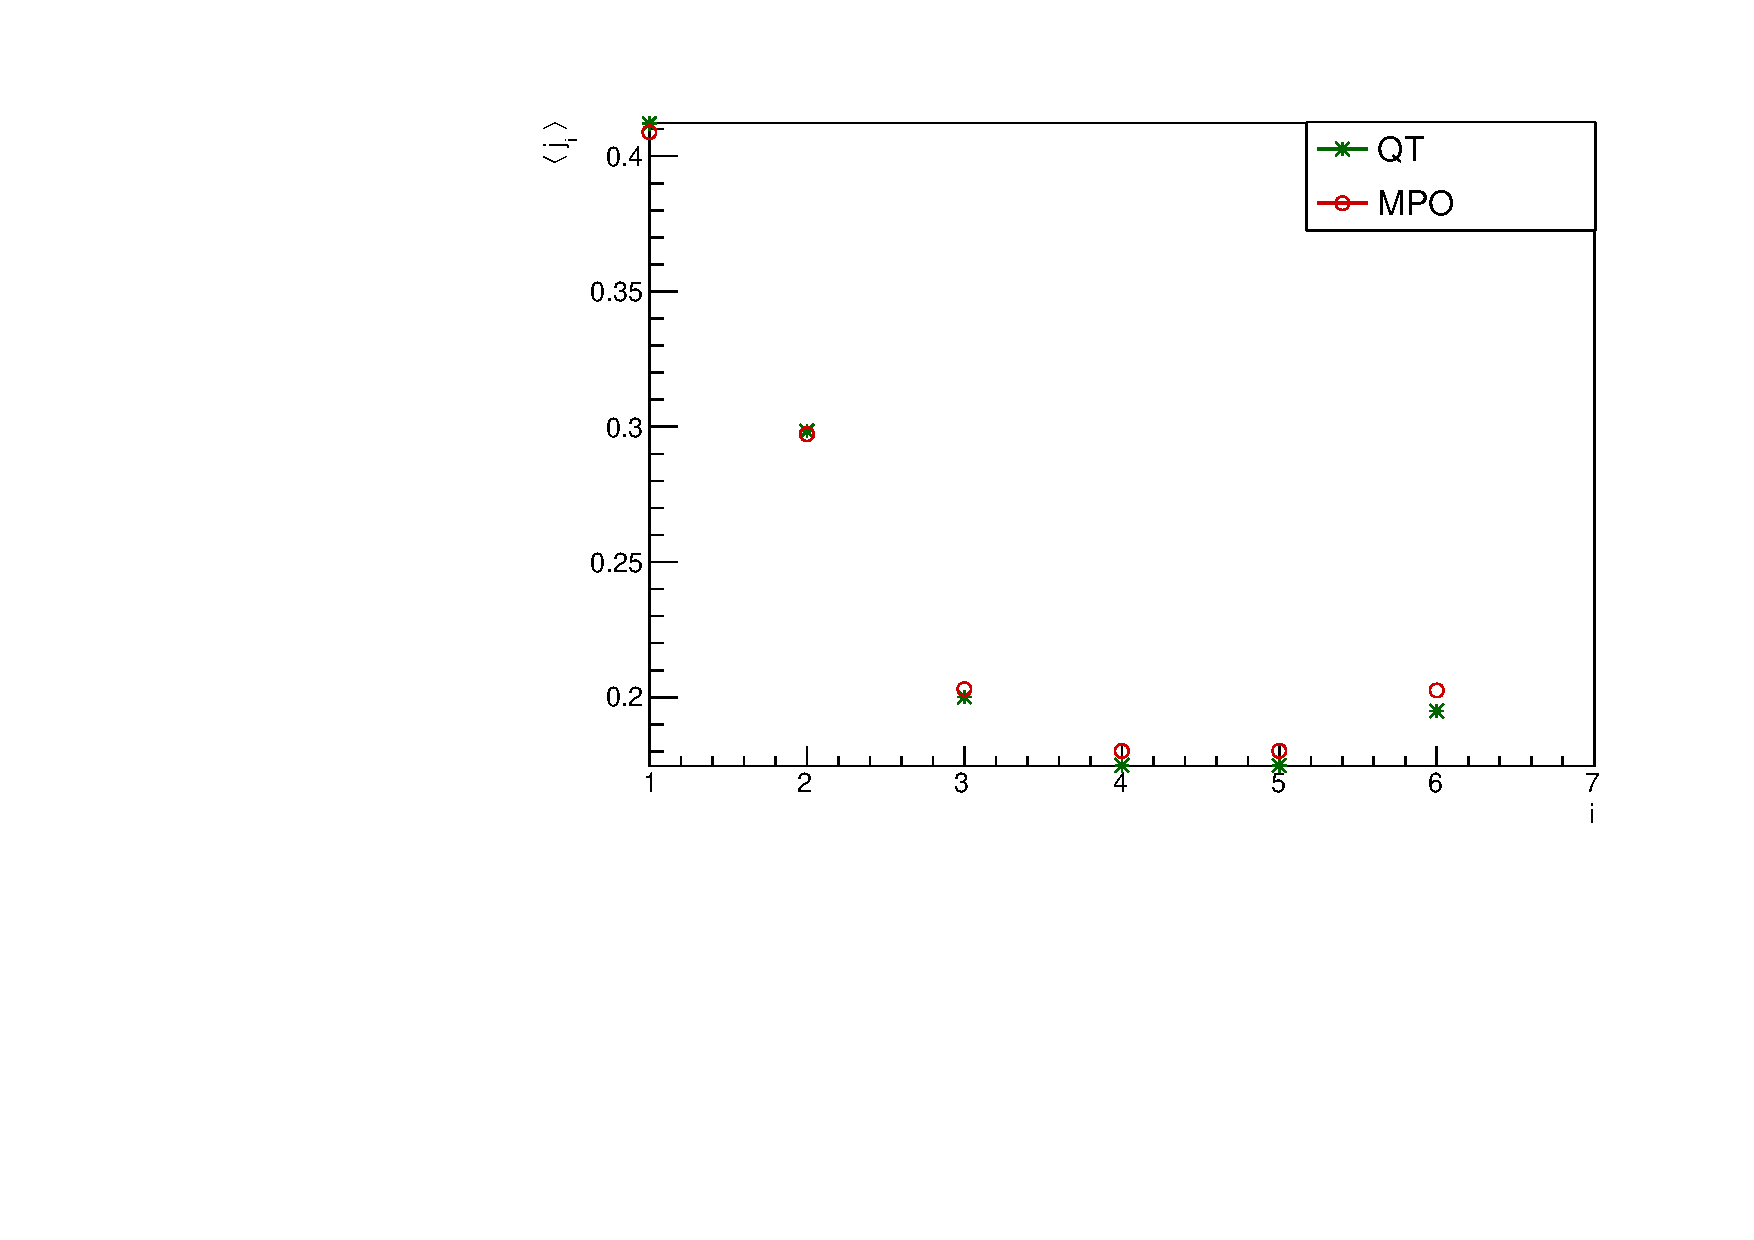
\includegraphics[scale=0.7]{Figures/8sites/SpinCurr_8s_J10505.pdf}
    %\caption{Spin current of the chain, characterized by $\gamma=1, J_x=1, J_y=0.5, %J_z=0.5$; \emph{i} stands for the site index.}
    %\label{fig:my_label}
%\end{figure}

%\begin{figure}[H]
    %\centering
    %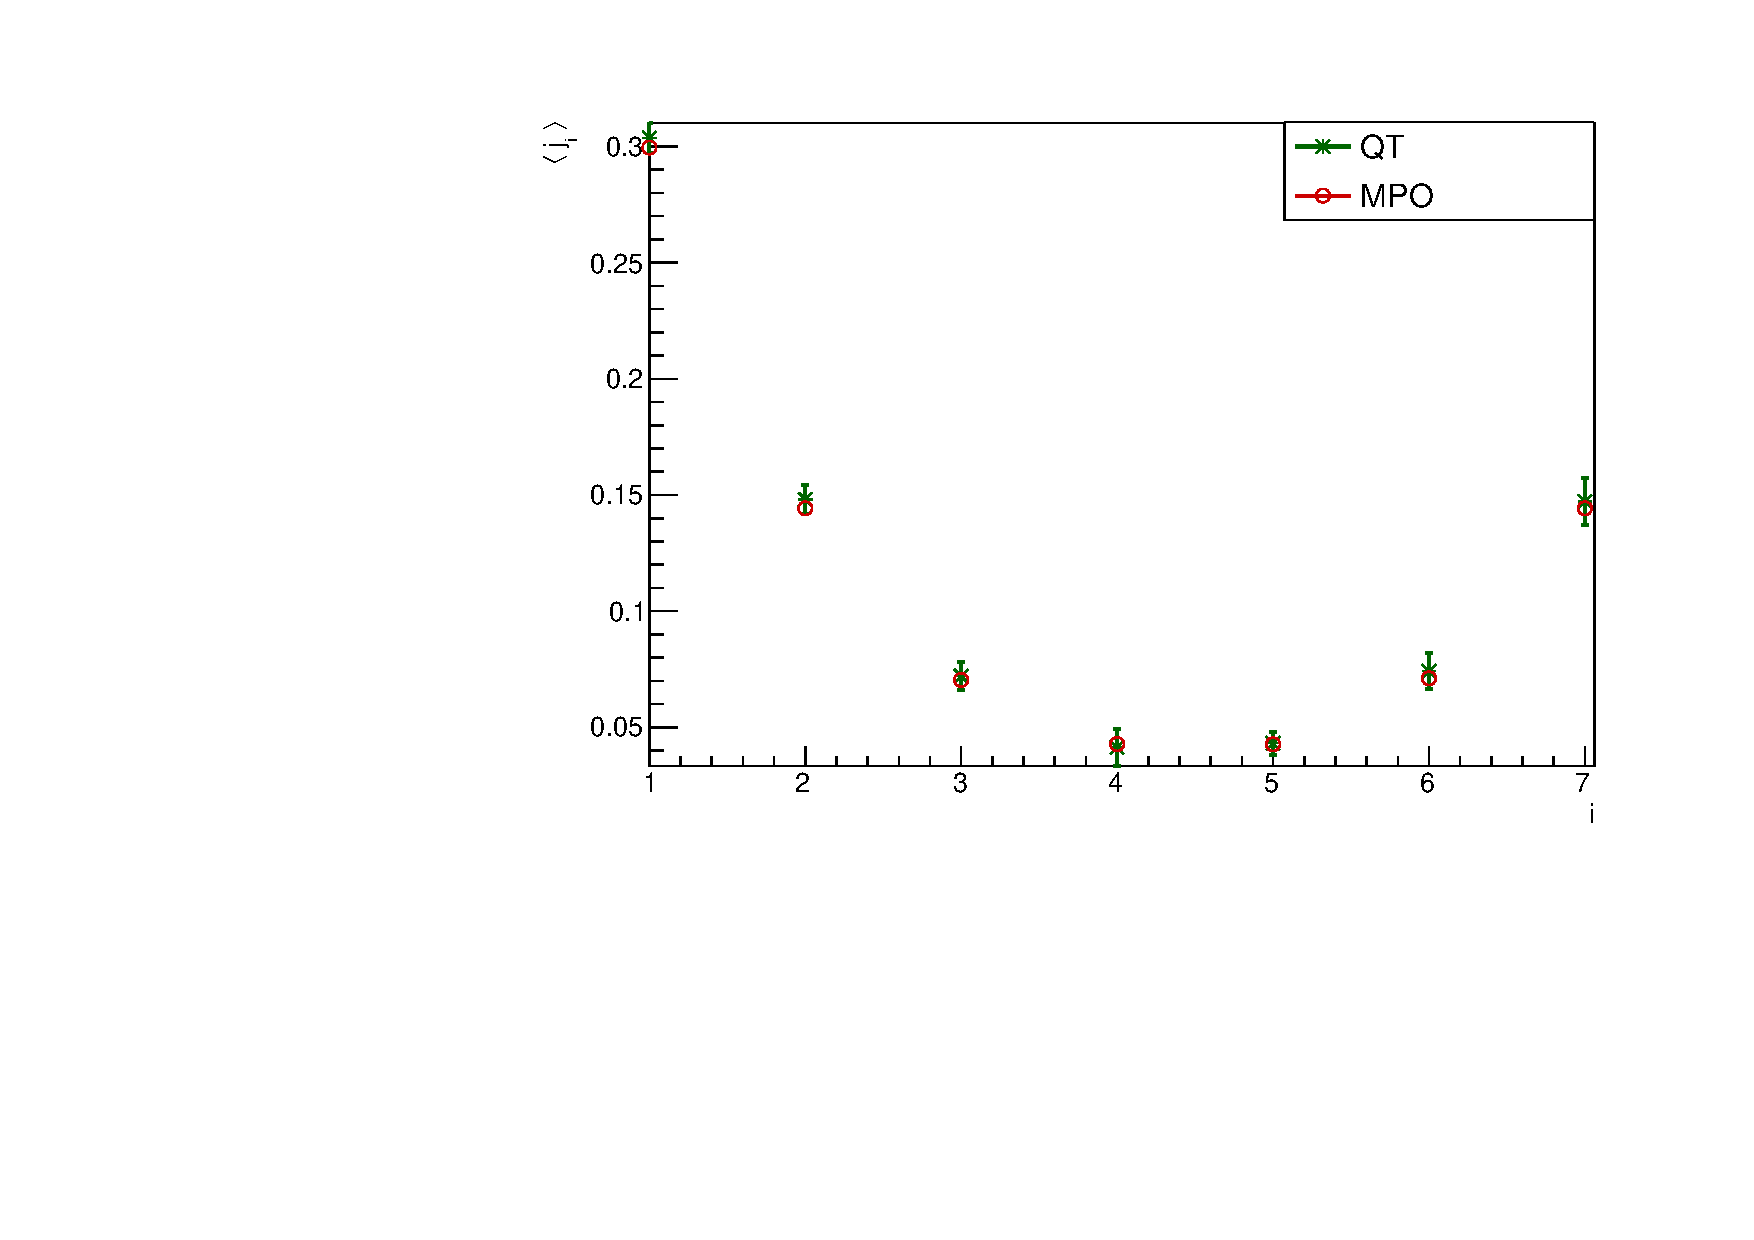
\includegraphics[scale=0.7]{Figures/8sites/SpinCurr_8s_J1051.pdf}
    %\caption{Spin current of the chain, characterized by $\gamma=1, J_x=1, J_y=0.5, %J_z=1$; \emph{i} stands for the site index.}
    %\label{fig:my_label}
%\end{figure}

%\begin{figure}[H]
    %\centering
    %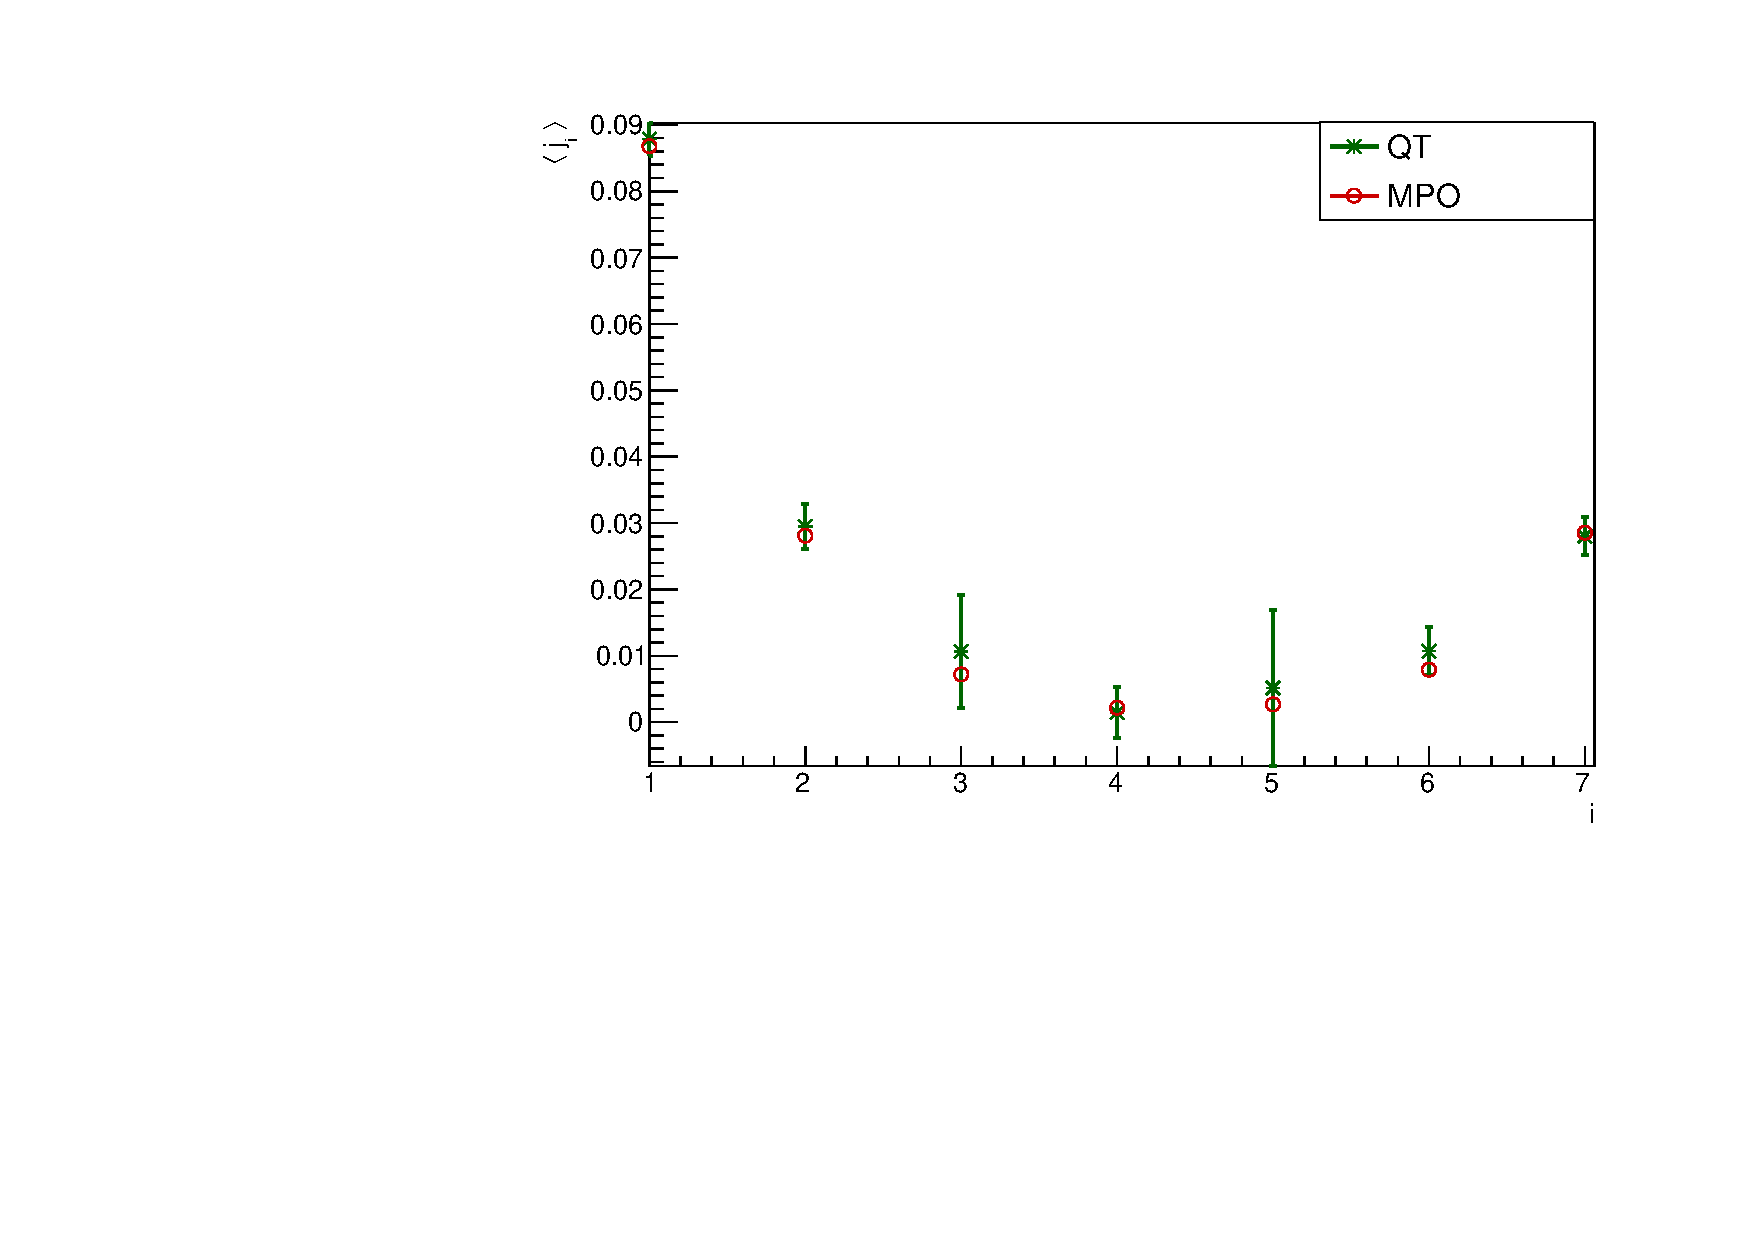
\includegraphics[scale=0.7]{Figures/8sites/SpinCurr_8s_J10515.pdf}
    %\caption{Spin current of the chain, characterized by $\gamma=1, J_x=1, J_y=0.5, %J_z=1.5$; \emph{i} stands for the site index.}
    %\label{fig:my_label}
%\end{figure}

%Let us see what happens in the case of a \textbf{12-sites} chain.
%
%\begin{figure}[H]
%    \centering
%    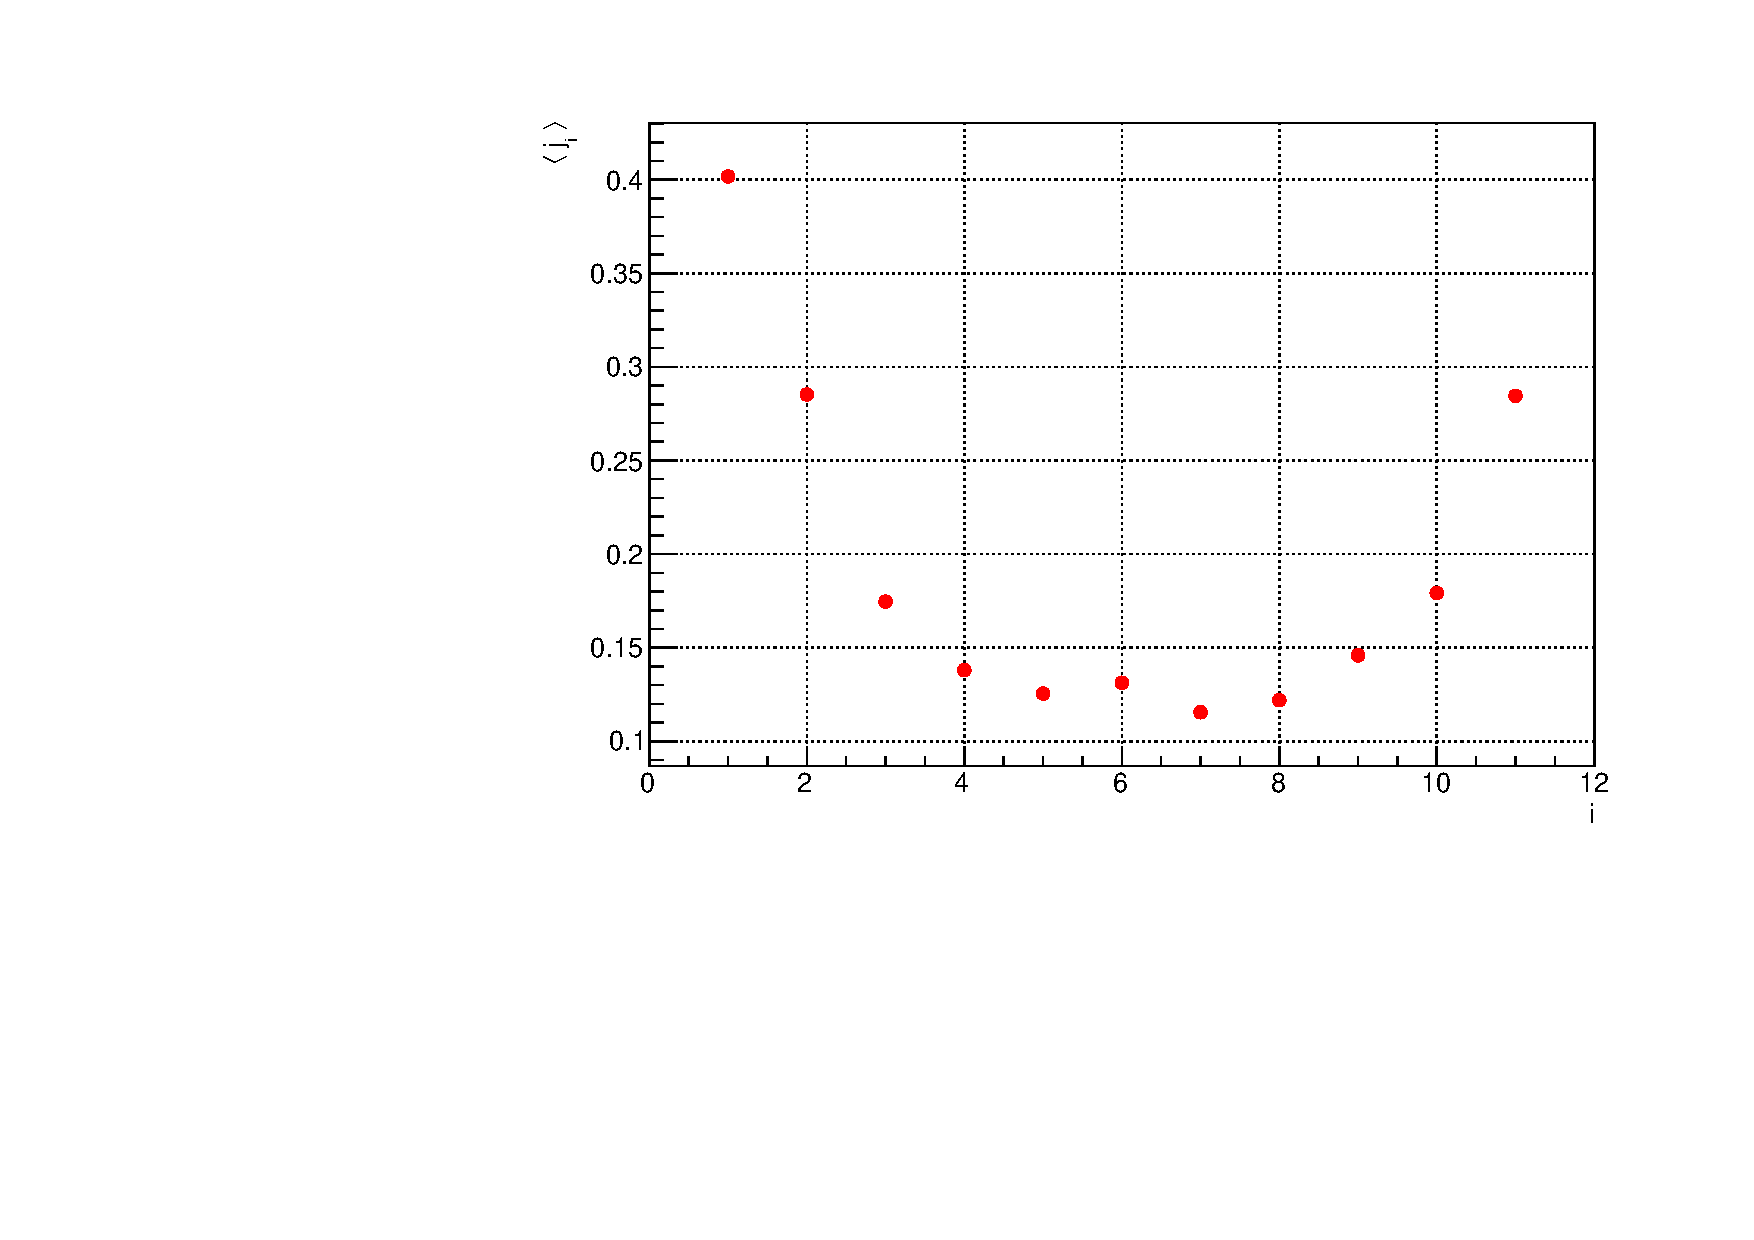
\includegraphics[scale=0.7]{Figures/12sites/SpinCurrL012m060Time002000_J10505.pdf}
%    \caption{Spin current of a 12-sites chain, characterized by $\gamma=1, J_x=1, J_y=0.5, J_z=0.5$; %\emph{i} stands for the site index. Data are obtained from MPO method.}
%    \label{fig:my_label}
%\end{figure}
%
%\begin{figure}[H]
%    \centering
%    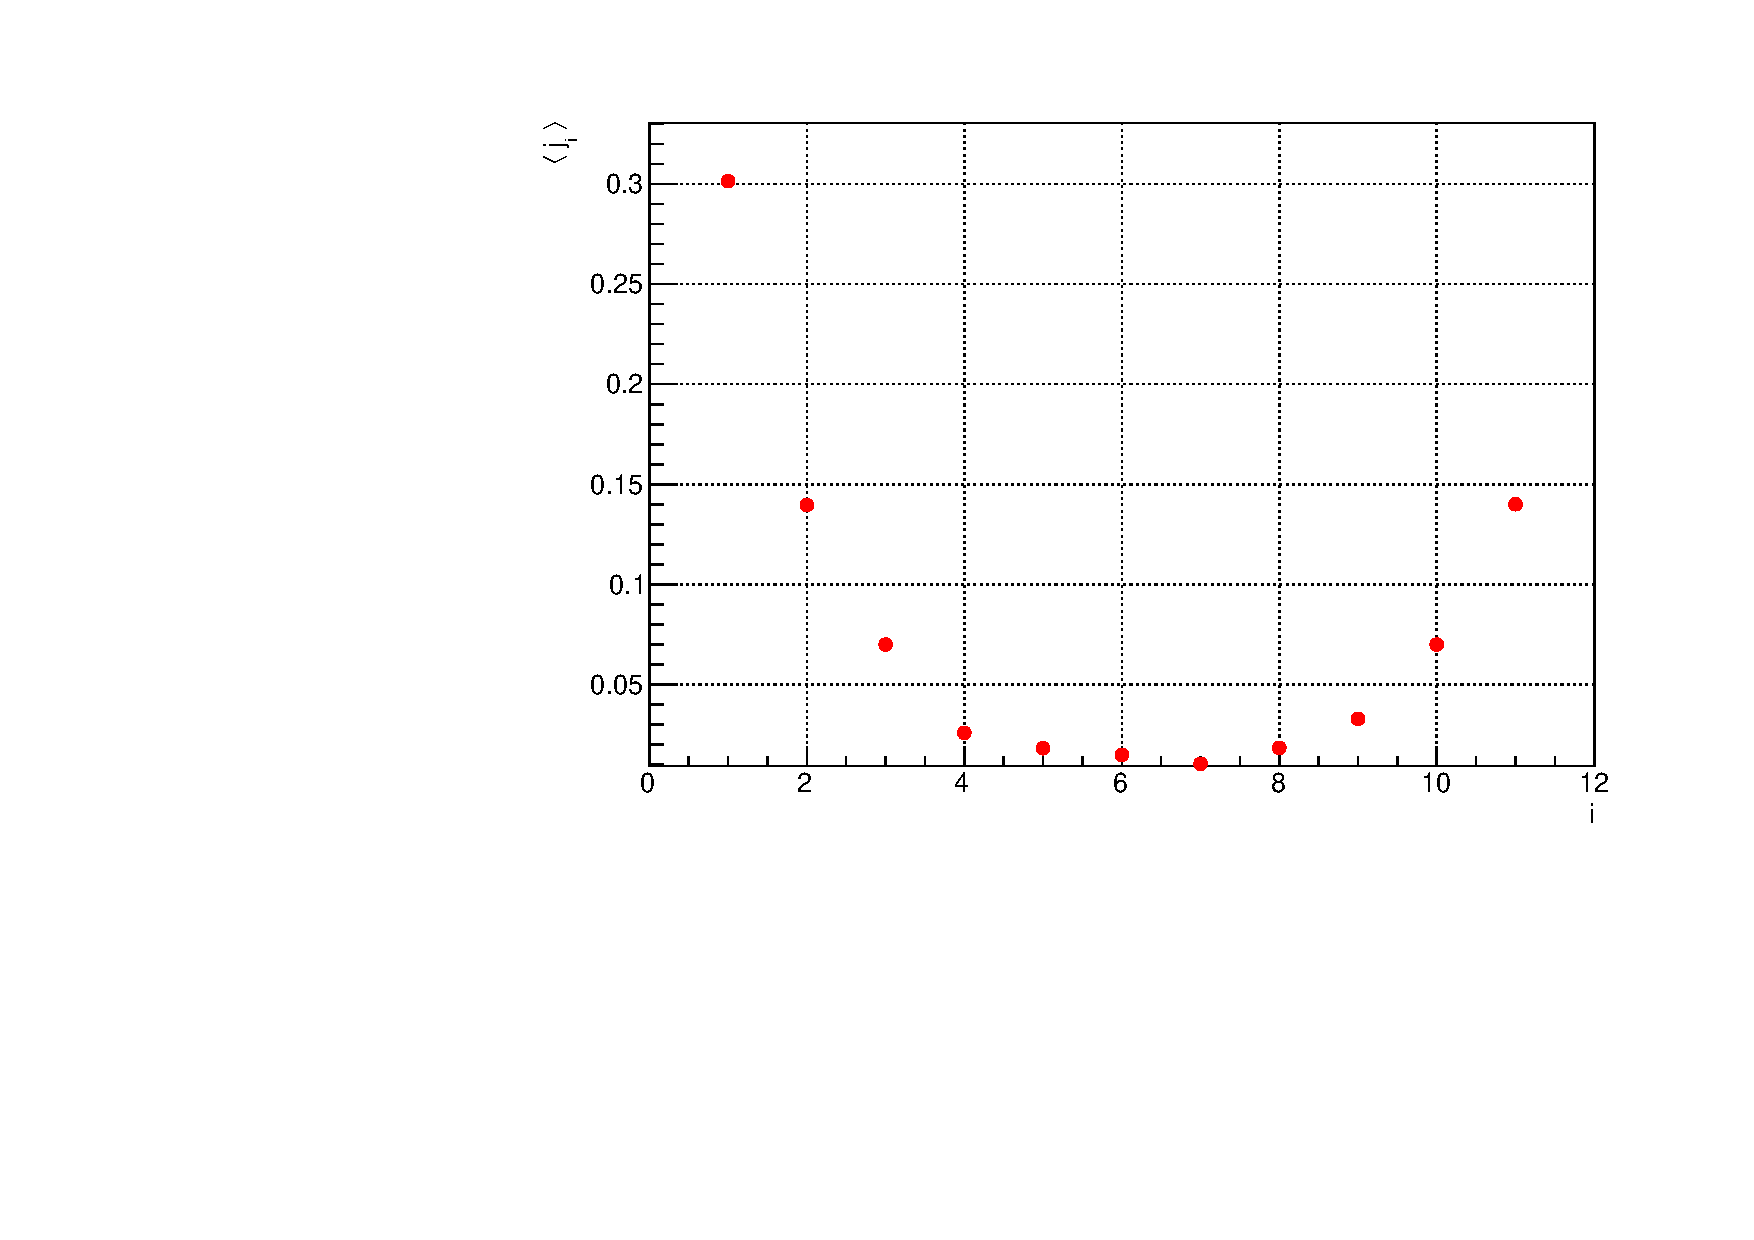
\includegraphics[scale=0.7]{Figures/12sites/SpinCurrL012m060Time002000_J1051.pdf}
%    \caption{Spin current of a 12-sites chain, characterized by $\gamma=1, J_x=1, J_y=0.5, J_z=1.$; %\emph{i} stands for the site index. Data are obtained from MPO method.}
%    \label{fig:my_label}
%\end{figure}
%
%\begin{figure}[H]
%    \centering
%    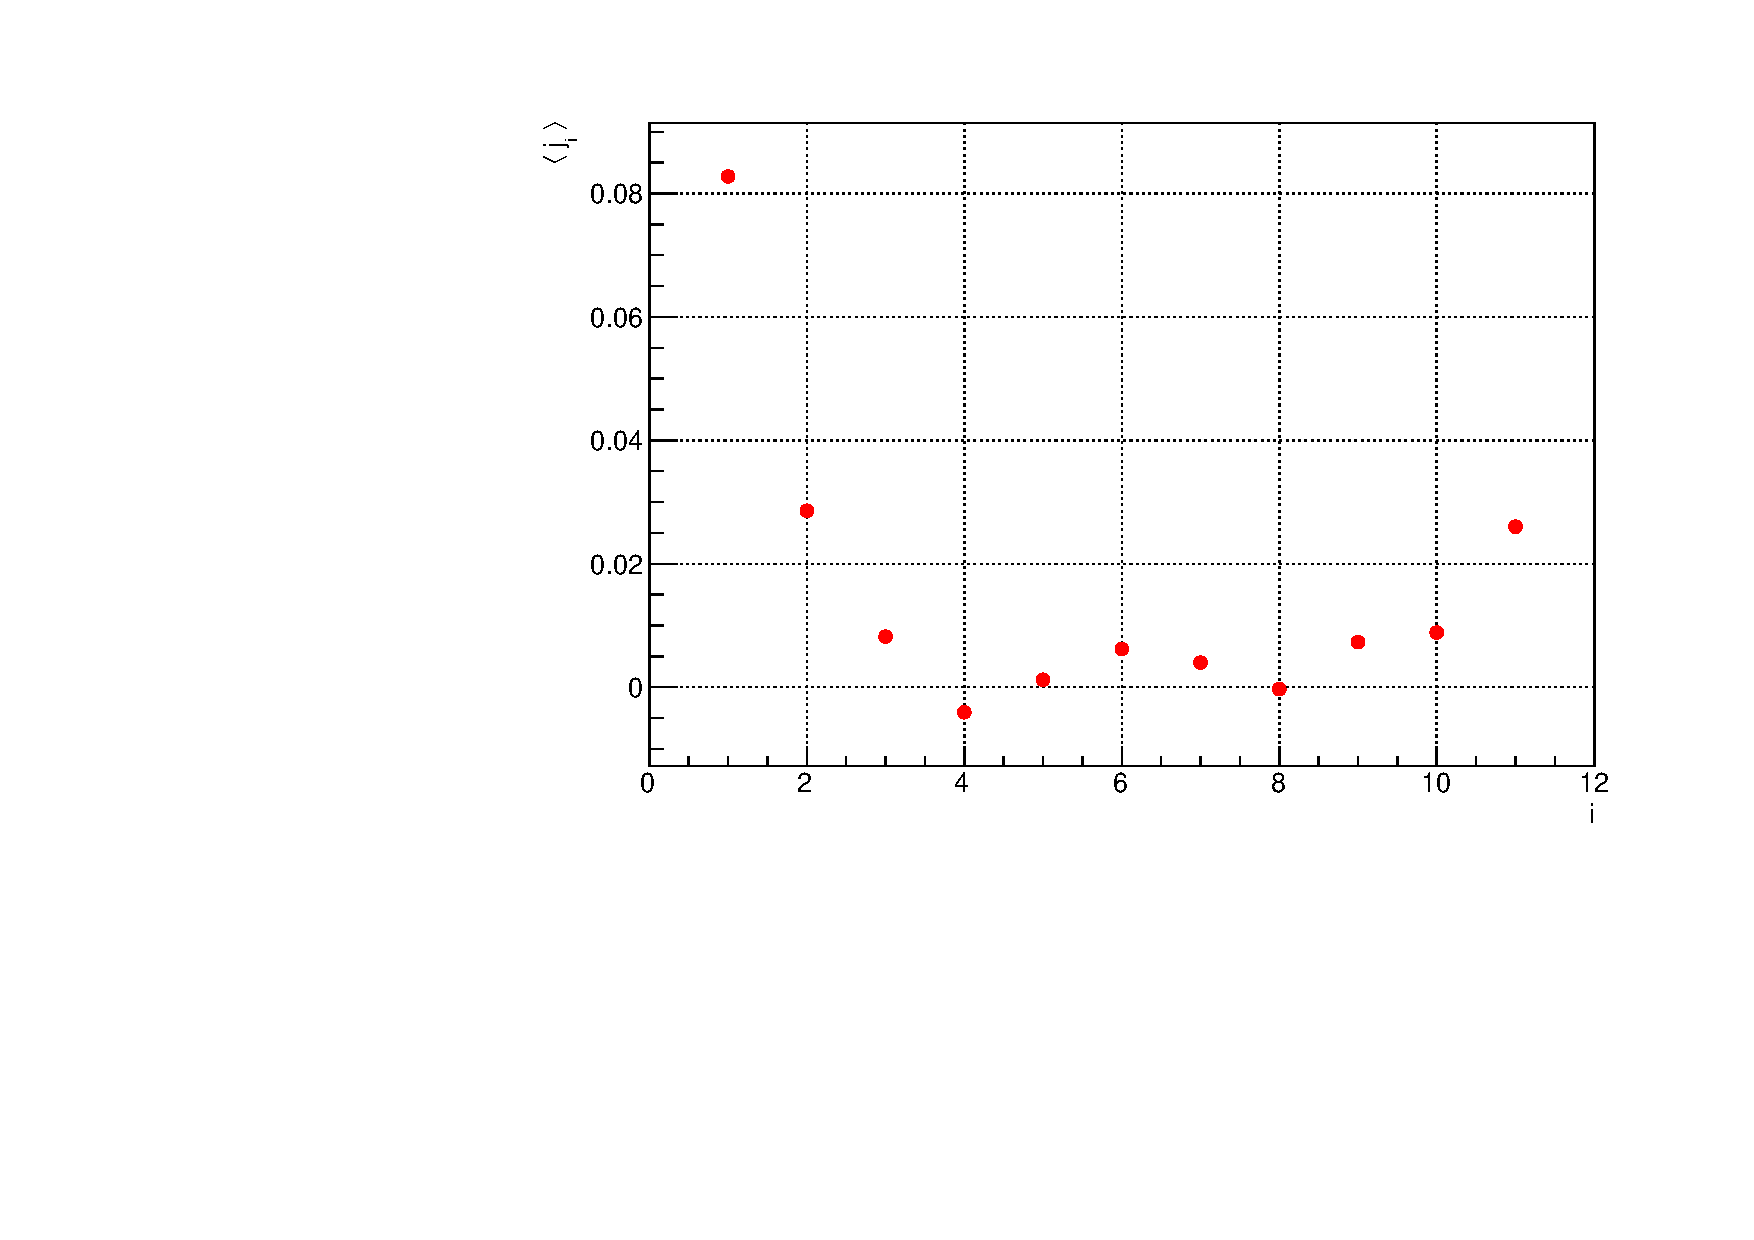
\includegraphics[scale=0.7]{Figures/12sites/SpinCurrL012m060Time002000_J10515.pdf}
%    \caption{Spin current of a 12-sites chain, characterized by $\gamma=1, J_x=1, J_y=0.5, J_z=1.5$; %\emph{i} stands for the site index. Data are obtained from MPO method.}
%    \label{fig:my_label}
%\end{figure}

As done previously for the observables already studied, we can see how the spin current changes for chain of different lengths with the same model. In the middle panel of fig.~\ref{fig:spinCurrVSsizeVSgamma} it is shown the spin current for a 8, 12 and 16-sites chain, characterized by $J_z = 1$ and dissipation rate $\gamma = 1$. The curves are asymmetric, due to the fact that the Heisenberg model XYZ has an intrinsic anisotropy. While the length of the chain increases, the spin current shows a flatter profile which is consistent with the fig.~\ref{fig:LM_comparisonVSsizeJz1Gamma1} where the plateau of null magnetization becomes bigger while the size of the chain grows.

An aspect worth considering is the common peak value of the spin current, independent of the chain size. As done in the section~\ref{sec:magn_profile} studying the magnetization profile, we can see how this value changes varying $\gamma$. 

In fig.~\ref{fig:spinCurrVSsizeVSgamma} we have kept the same scale of y-axis: this allows to note that the spin current between the first to spin of the chain, increases while $\gamma$ grows. 

\begin{figure}[H]
\centering
    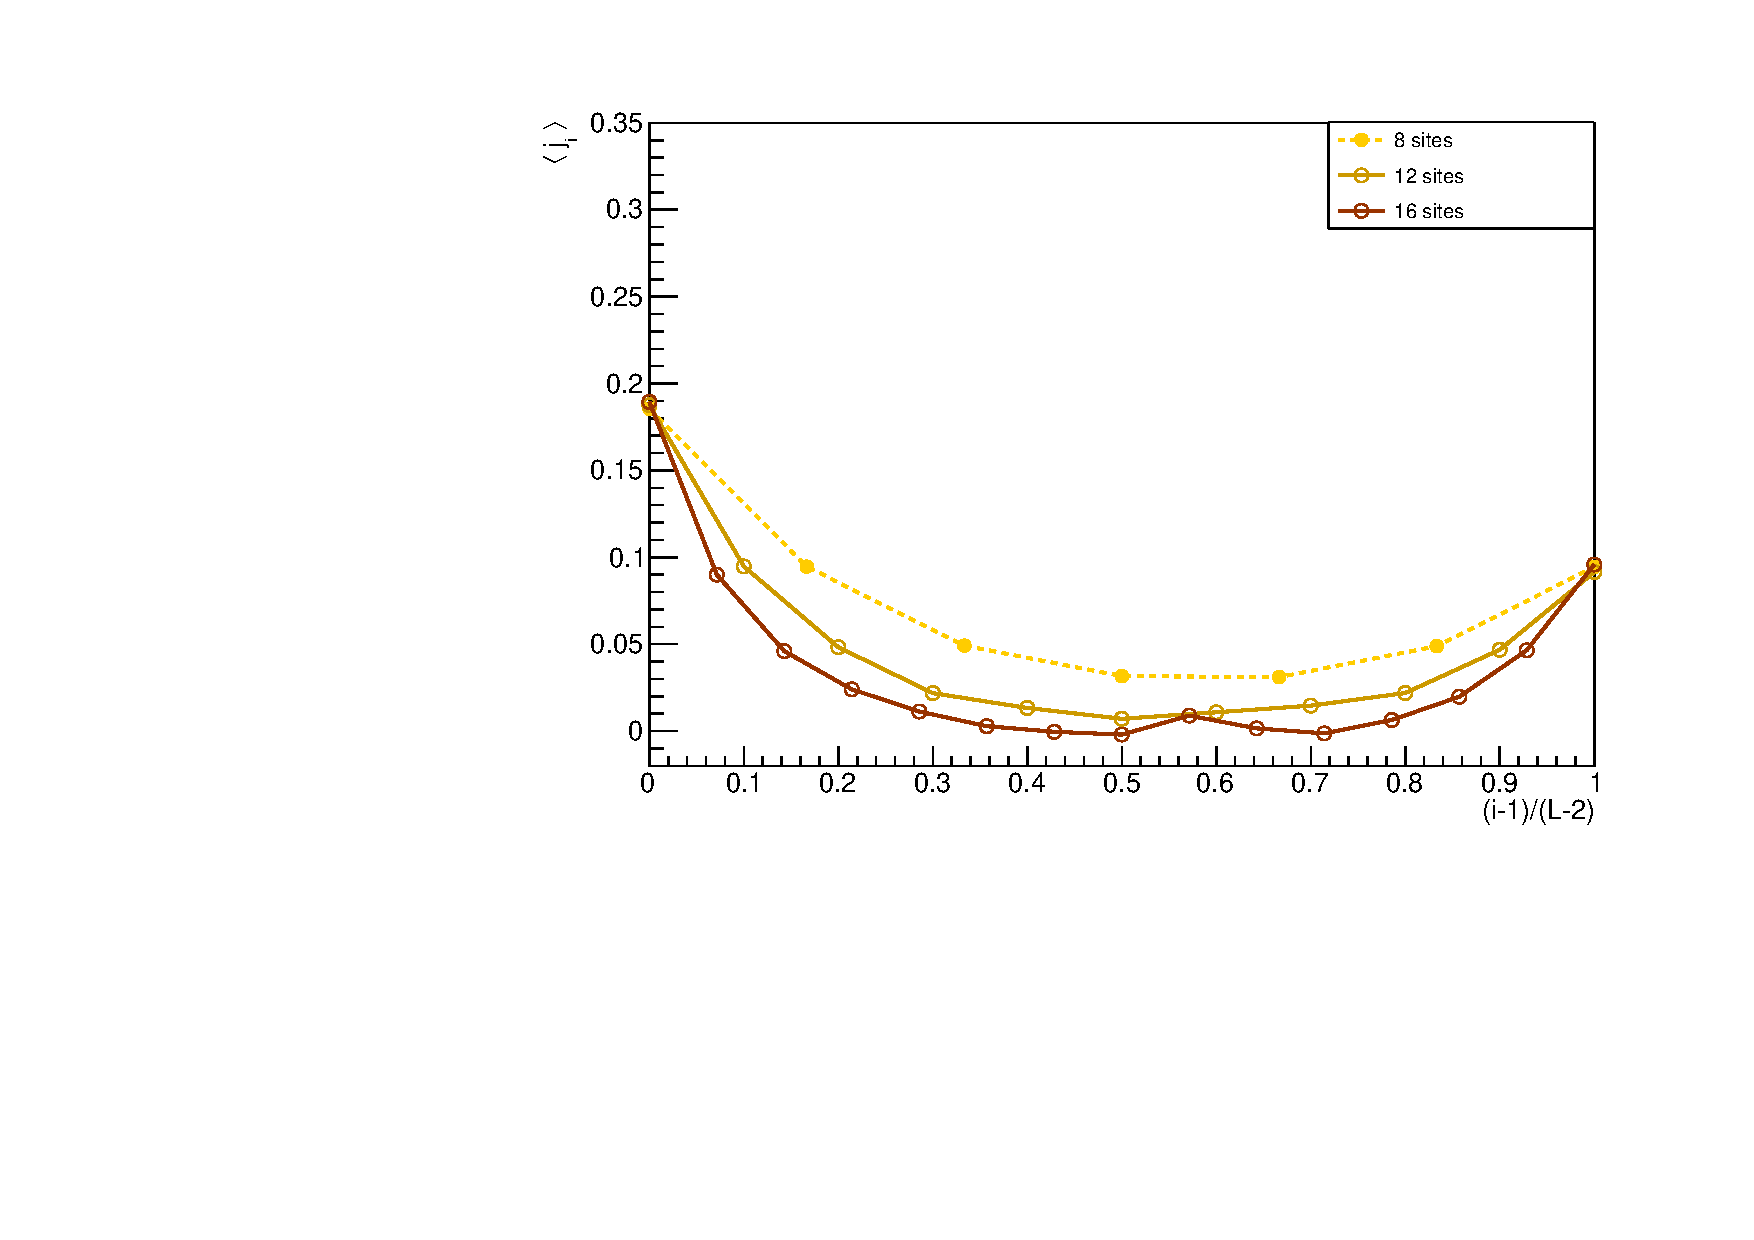
\includegraphics[scale=0.55]{Figures/spinCurrVSsize_Gamma05.pdf}
    \label{fig:8sites_LMvsGamma}
    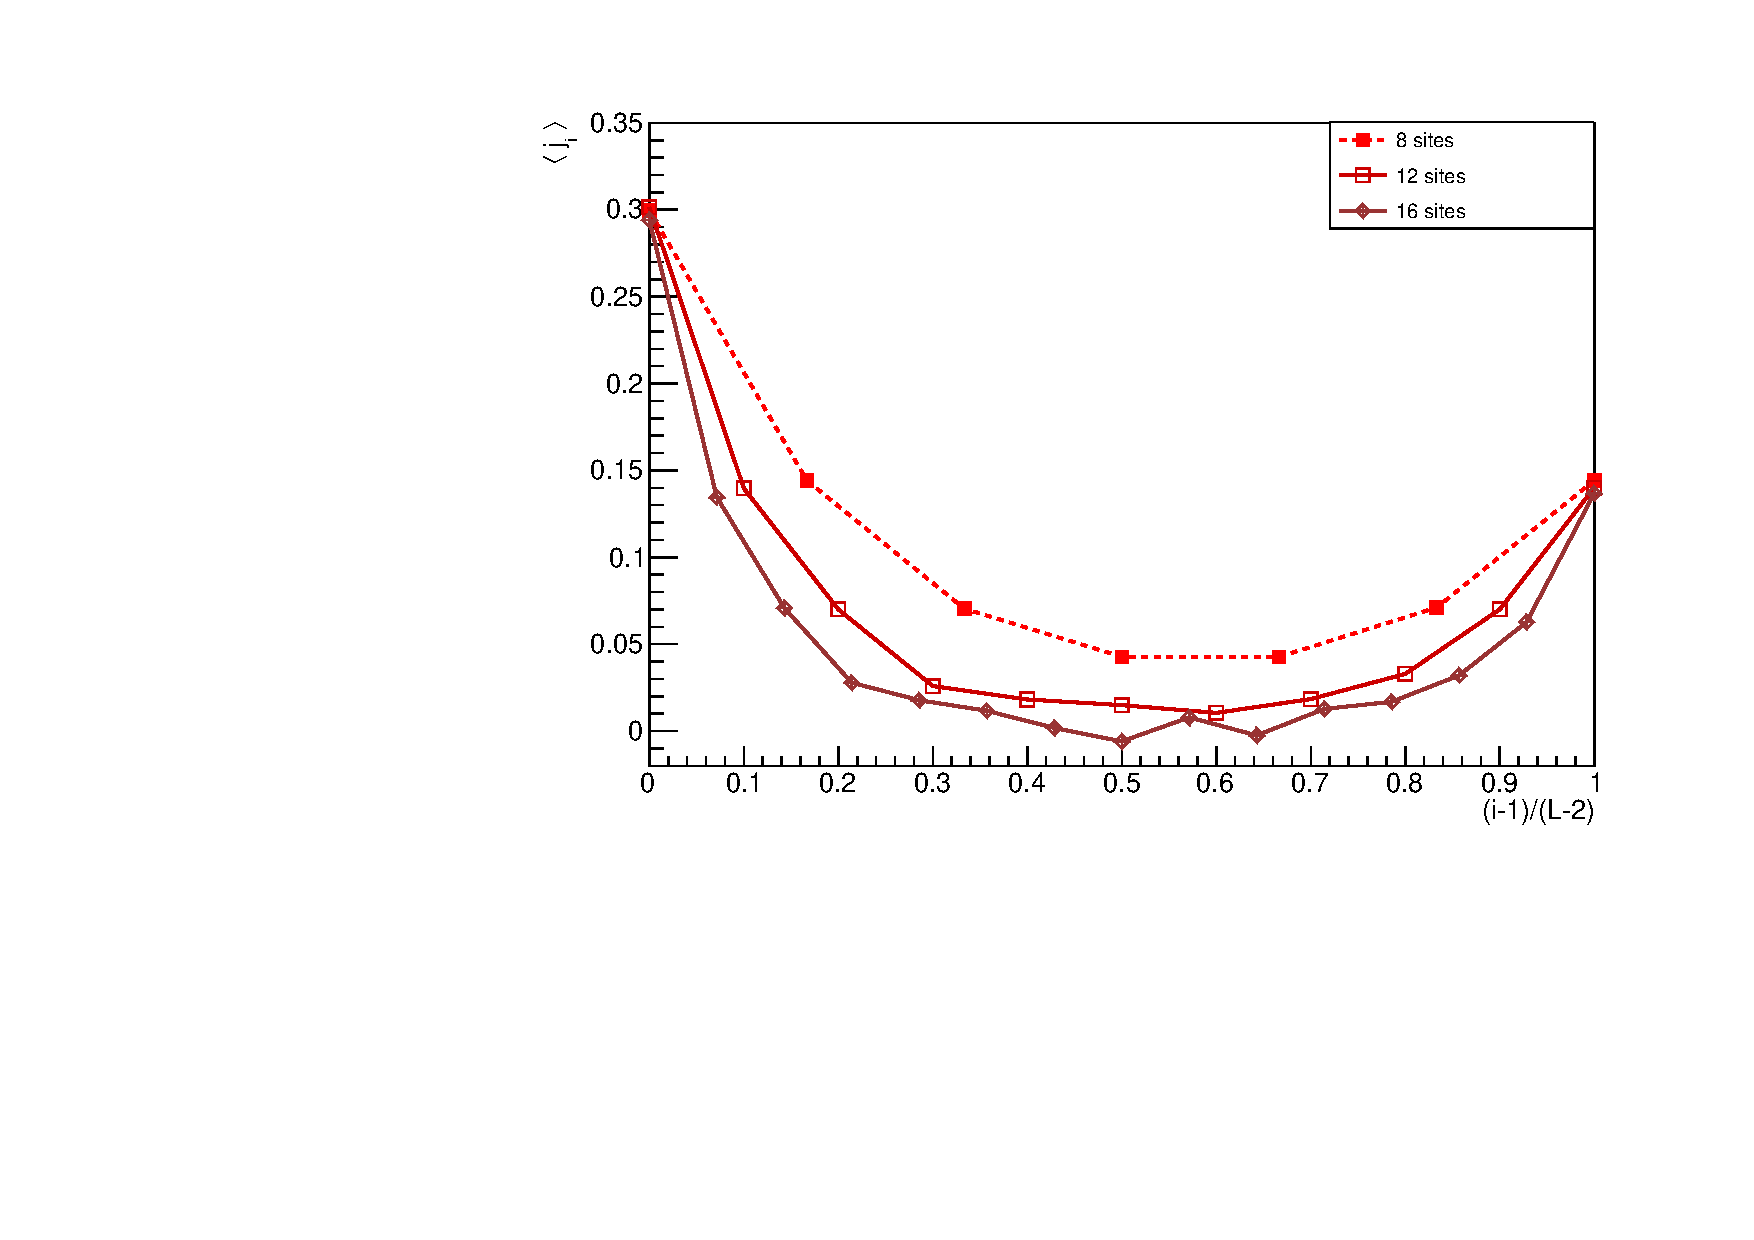
\includegraphics[scale=0.55]{Figures/spinCurrVSsize_Gamma1.pdf}
    \label{fig:12sites_LMvsGamma}
    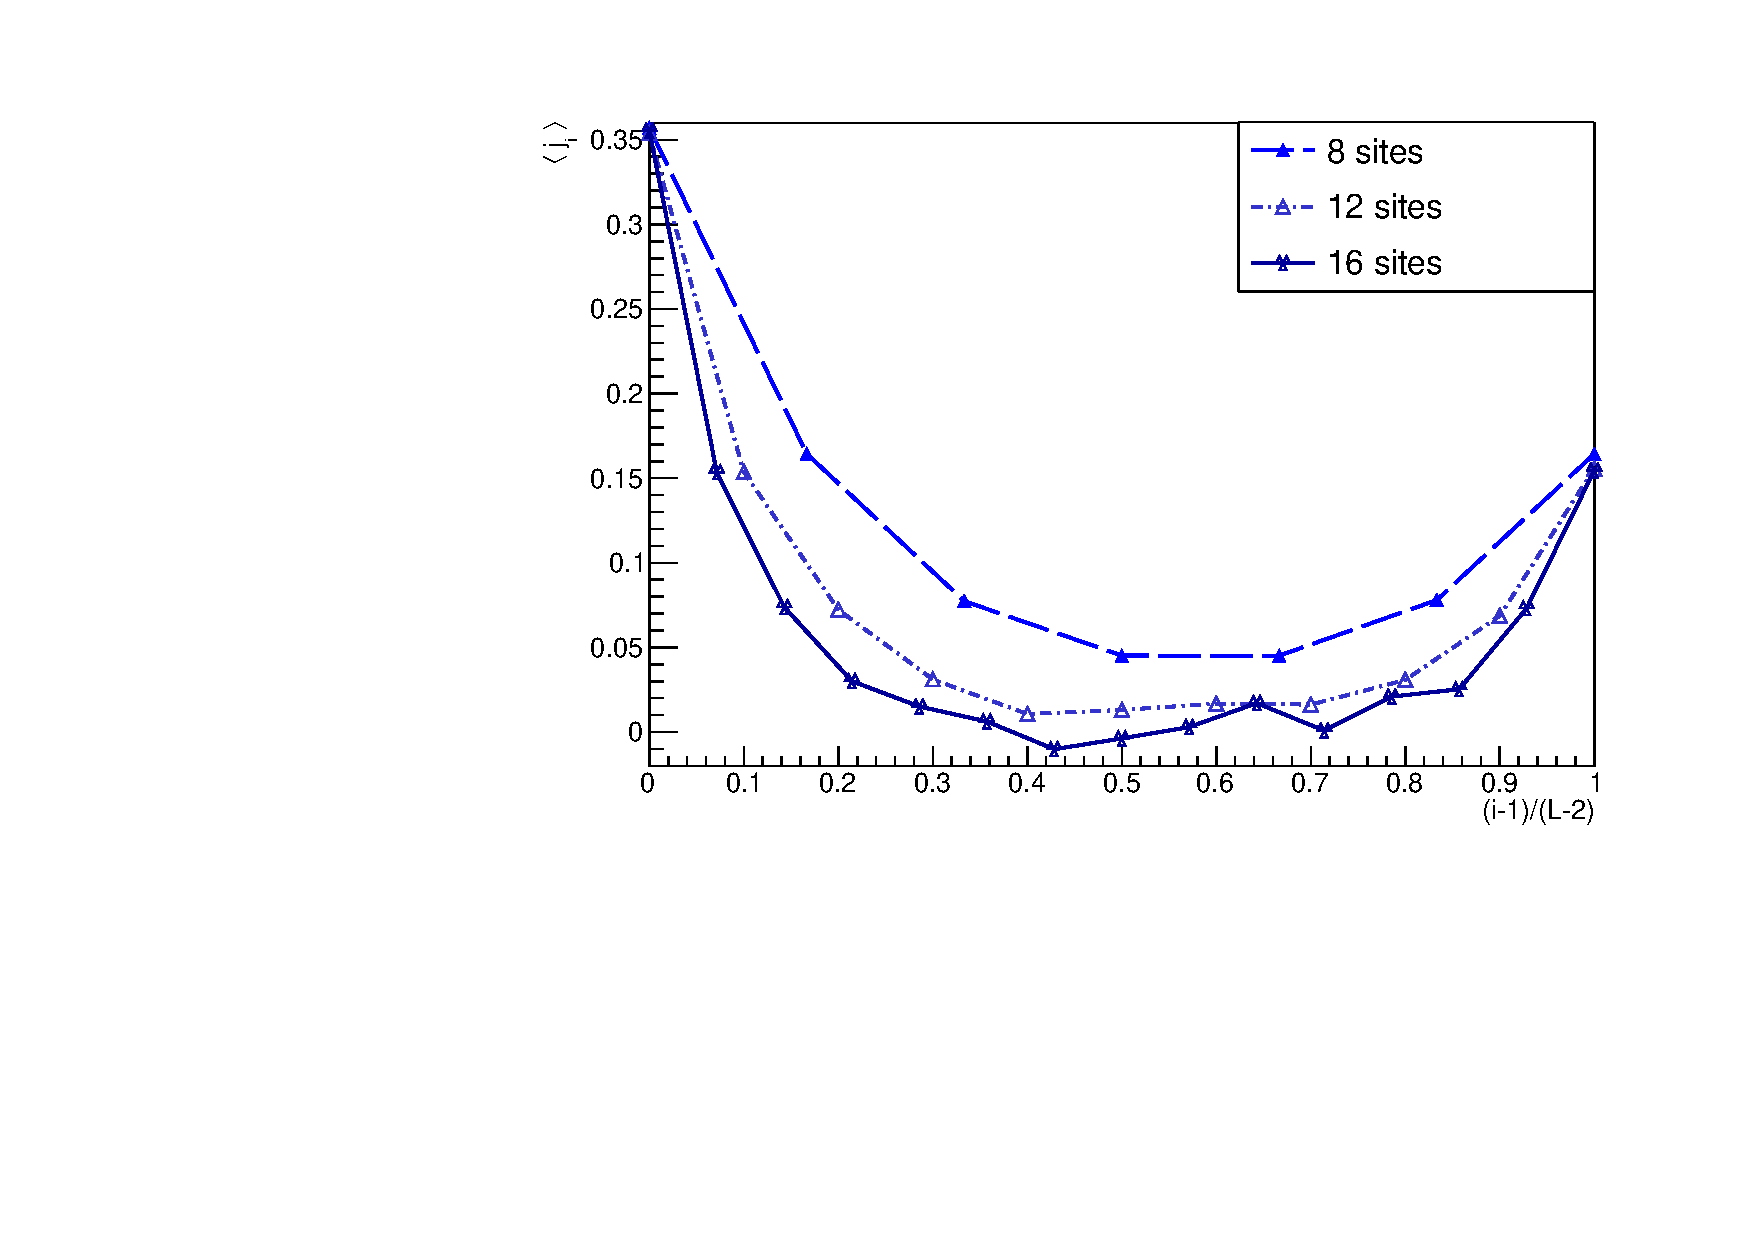
\includegraphics[scale=0.55]{Figures/spinCurrVSsize_Gamma15.pdf}
    \label{fig:16sites_LMvsGamma}
\captionsetup{width=1.\linewidth}
\caption{Spin current for $\gamma = 0.5$ (upper panel), $\gamma = 1$ (middle panel), $\gamma = 1.5$ (bottom panel) and $J_z = 1$ are shown. In every panel, a comparison between different chain lengths is done. Data are obtained from MPO method.}
\label{fig:spinCurrVSsizeVSgamma}
\end{figure}

It is interesting noting that the peak values reach a maximum and then decrease, following a non-monotonic trend, as shown in fig.~\ref{fig:PeakValueSpinCurrVSgamma_8sites}. This can be explained observing that there is a competition between two effects: the dissipation and the Hamiltonian of the system. If these two dynamics are characterized by the same magnitude, the regime becomes the one shown in the figure, with a non-trivial trend. However, if the effect of dissipation acquires a more important role over the Hamiltonian dynamics, the spin-flip is inhibited and there is no more transport of information: the system will be paralyzed in the configuration dictated by the dissipators. Instead, if the dissipation is too small, it cannot create correlations, so the spin transport will be zero. It is worth observing that having a maximum in the spin current, i.e. a non-trivial trend, would not have been possible if there was only dissipation or only the Hamiltonian dynamics; the trend in fig.~\ref{fig:PeakValueSpinCurrVSgamma_8sites} is only possible because of the competition between them.

%analyzing the curve. First of all, for small values (i.e. $\gamma \sim 0.5$) there is a non-null spin current; as said, for a certain value of $\gamma$ the spin current reaches the maximum value and then begins to decrease tending asymptotically to zero. While $\gamma$ grows, the dissipation acquires a more important role over the Hamiltonian dynamics, the system is driven so that its spin current is zero. This is consistent with the trend shown in fig.~\ref{fig:LM_PeakAnd4th_vsGamma2panels} of the positive peak value of $\langle \sigma^z \rangle$ and of the value of $\langle \sigma^z \rangle$ for the forth site of the chain, in which while $\gamma$ increases the magnetization tends asymptotically to a constant value. 

\begin{figure}[H]
    \centering
    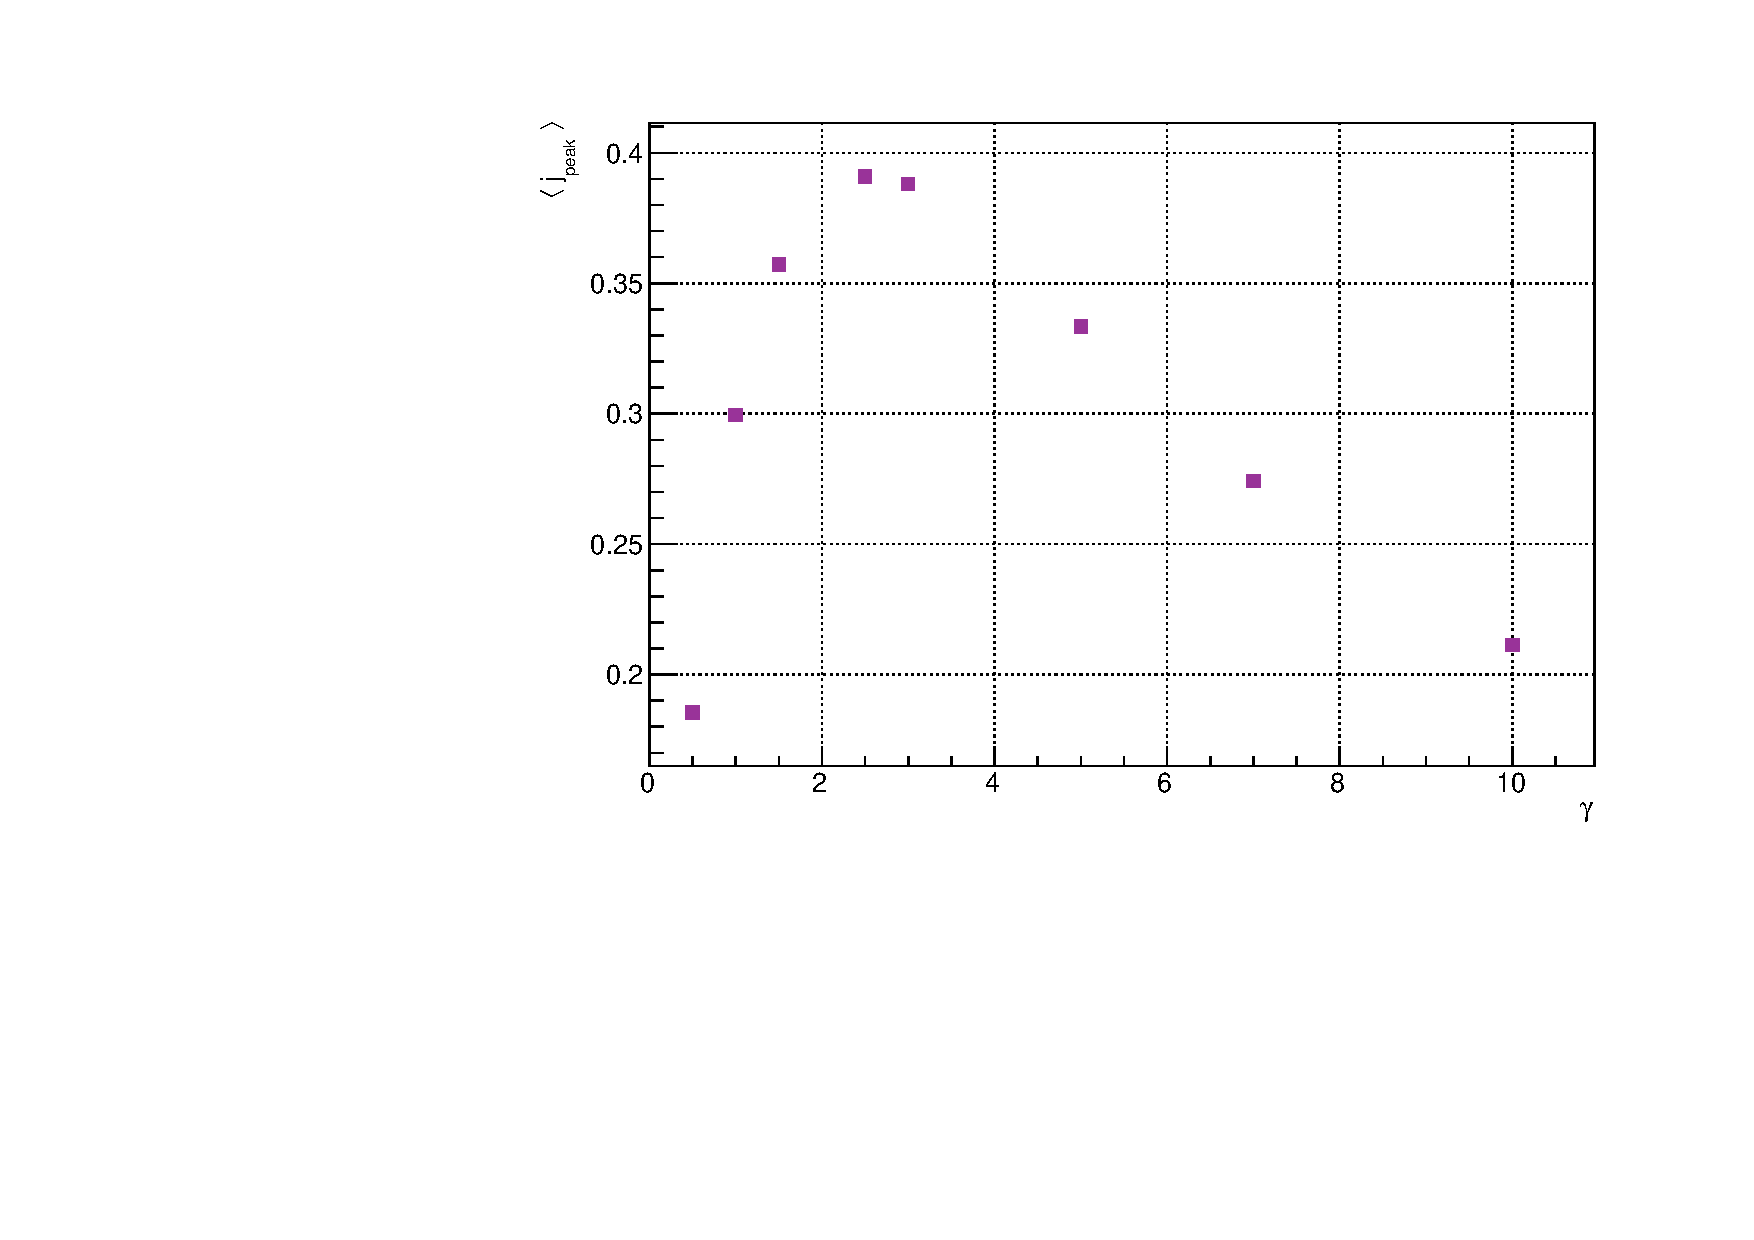
\includegraphics[scale=0.7]{Figures/PeakValueSpinCurrVSgamma_8sites.pdf}
    \captionsetup{width=1.\linewidth}
    \caption{Peak values of spin current for several values of $\gamma$. Data are obtained from MPO method.}
    \label{fig:PeakValueSpinCurrVSgamma_8sites}
\end{figure}


%%%%%%%%%%%%%%%%%%%%%%%%%%%%%%%%%%%%%%%%%%%%%%%%%%%%%%%%%%%%%%%%%%
%%%%%%%%%%%%%%%%%%%%%%%%%%%%%%%%%%%%%%%%%%%%%%%%%%%%%%%%%%%%%%%%%%
%%%%%%%%%%%%%%%%%%%%%%%%%%%%%%%%%%%%%%%%%%%%%%%%%%%%%%%%%%%%%%%%%%
\section{A Conjectured Nonequilibrium Phase Transition}
\label{chapt4_phase_trans}

In an open system, the competition between unitary Hamiltonian evolution and dissipation can induce a dissipative phase transition for the steady state, as discussed for example in the case of spin systems by~\cite{phase_trans_spin_system}.
A phase transition is an important phenomenon in condensed-matter physics and can happens tuning one or more parameters of the Hamiltonian of the system. 

So far, we have studied the behaviour of 8, 12 and 16-sites chain varying the coefficient of dissipation rate $\gamma$. In this chapter, we focus on the behaviour of a 16-sites chain under a variation of $J_z$ will be investigated. Ideally, in order to discuss phase transition one should study an infinite-size chain; for this reason, the only chain under consideration will be the one with the biggest size between the ones analyzed in the present work.

First of all, we have analyzed the spin current under the variation of the coupling constant $J_z$. In fig.~\ref{fig:16sites_SpinCurrVaryingJz} the spin current for several values of $J_z$ is displayed. Some consideration can be made in regards to this plots.

%This behaviour is confirmed by the data obtained from QT method (fig.~\ref{fig:8sites_spinCurrVSJzQT}).

%\begin{figure}[H]
    %\centering
    %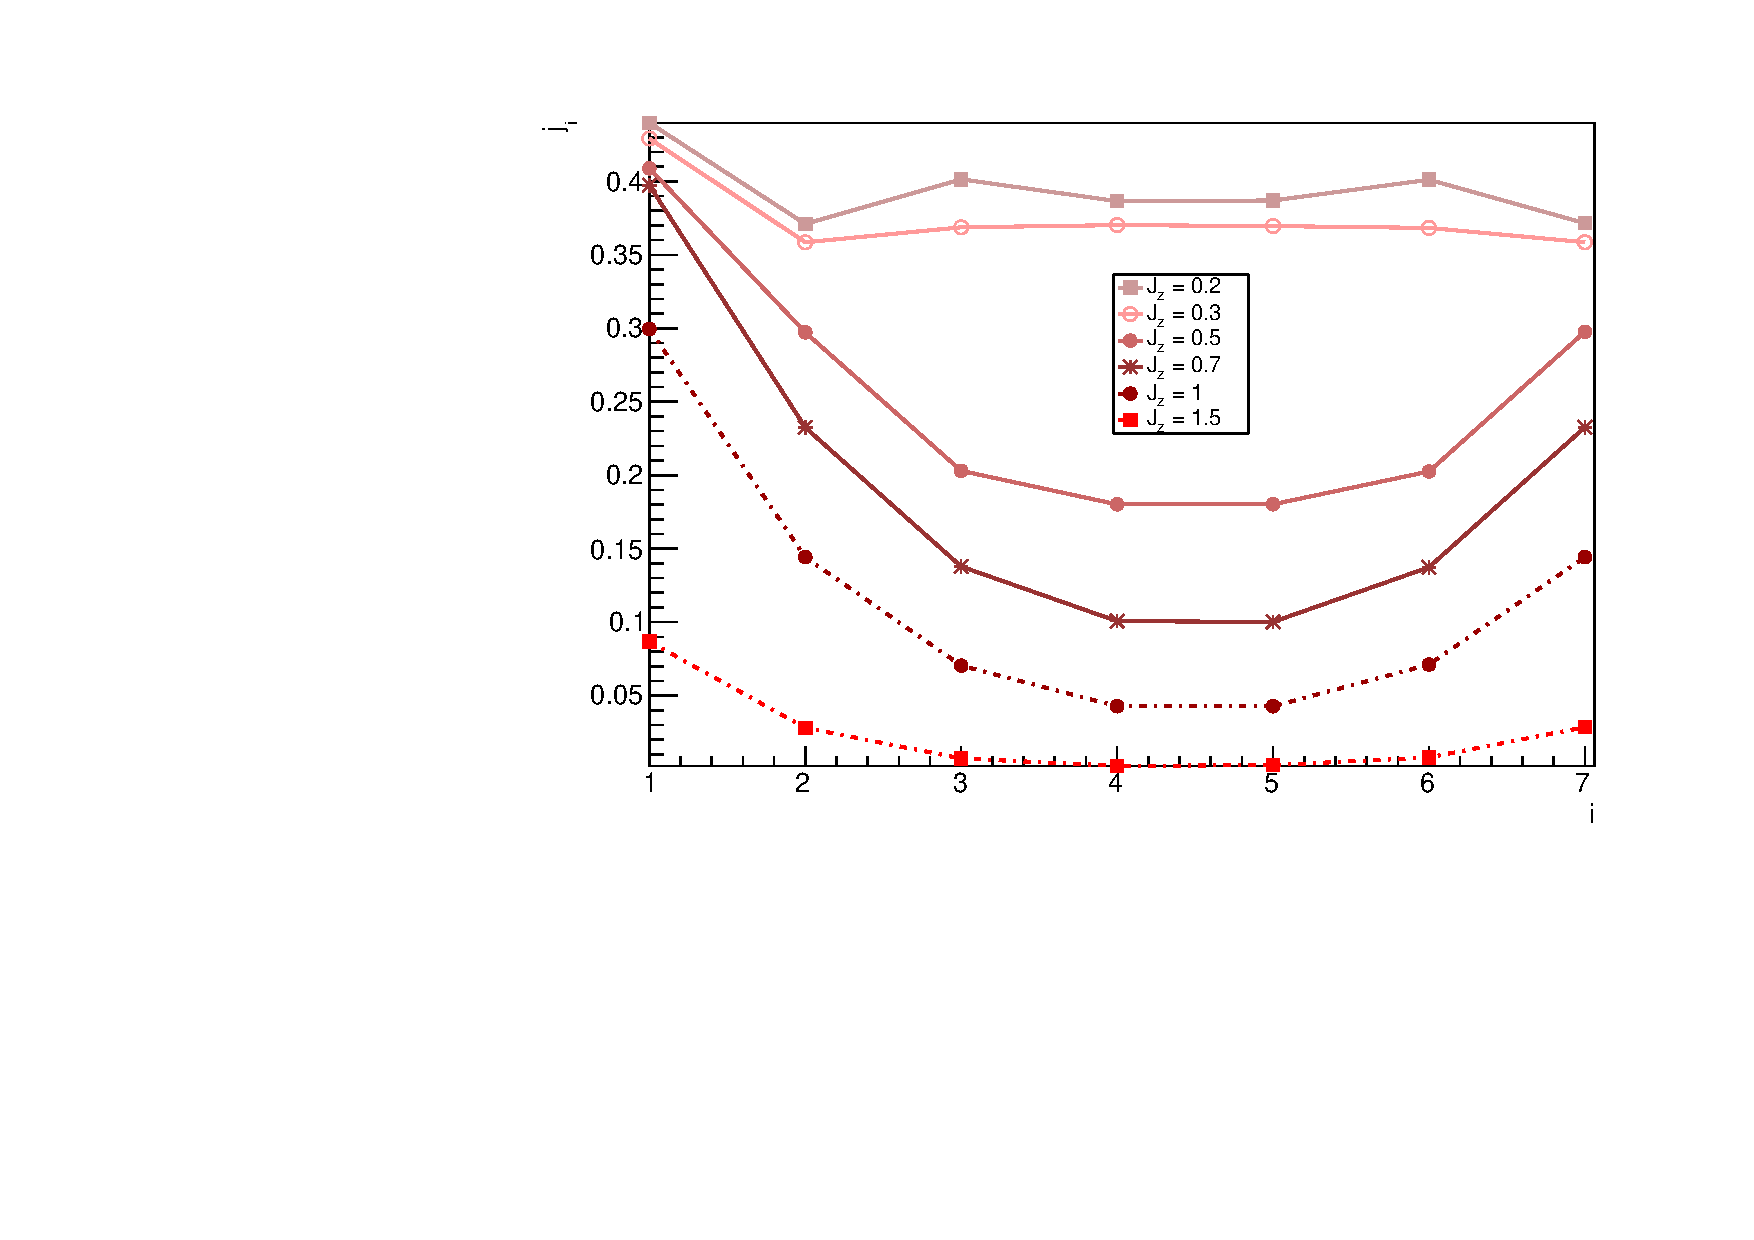
\includegraphics[scale=0.7]{Figures/8sites_spinCurrVSJz.pdf}
    %\caption{Spin current of a 8-sites chain, with $\gamma = 1$ for several values of $J_z$. Data %obtained from MPO method.}
    %\label{fig:8sites_spinCurrVSJz}
%\end{figure}

%\begin{figure}[H]
    %\centering
    %\includegraphics[scale=0.7]{Figures/8sites/8sites_spinCurrVSJz%QT.pdf}
    %\captionsetup{width=1.\linewidth}
    %\caption{Spin current of a 8-sites chain, with $\gamma = 1$ %for several values of $J_z$. Data obtained from QT method.}
    %\label{fig:8sites_spinCurrVSJzQT}
%\end{figure}

\begin{figure}[H]
    \centering
    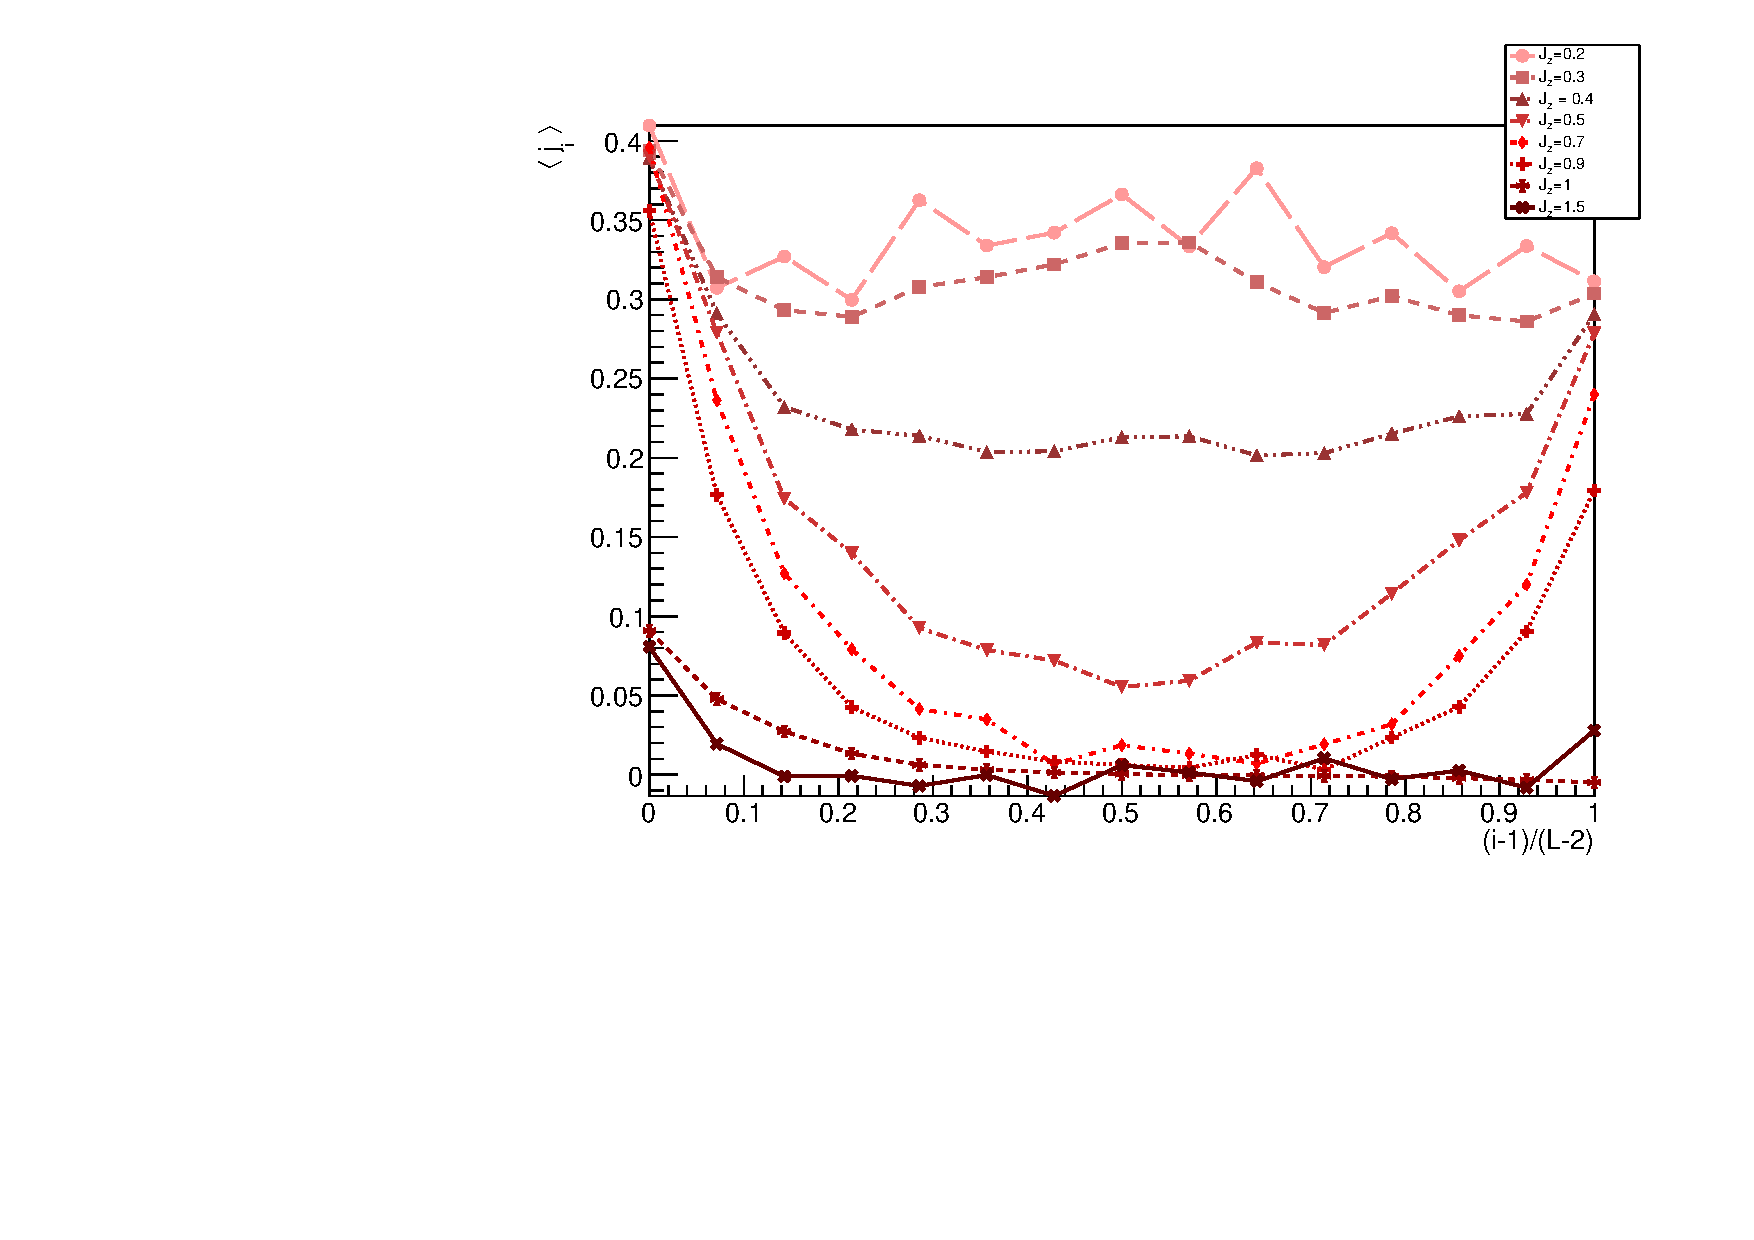
\includegraphics[scale=0.7]{Figures/16sites/16sites_SpinCurrVaryingJz.pdf}
    \captionsetup{width=1.\linewidth}
    \caption{Spin current of a 16-sites chain, with $\gamma = 1$ for several values of $J_z$. Data obtained from MPO method.}
    \label{fig:16sites_SpinCurrVaryingJz}
\end{figure}

The spin current between the first and the last two sites is independent from $J_z$, for $J_z < 1$; this can be a sign of the prevalence of dissipation over the Hamiltonian dynamics. Otherwise, for $J_z \geq 1$ the peak values (i.e. the spin current between the first two and the last two sites of the chain) drop while $J_z$ increases; this can be a sign of the growing prevalence of the Hamiltonian over the dissipation, while the coupling $J_z$ grows.

For the small values of $J_z$, i.e. for $J_z < 0.5$, the $\sigma_i^z\sigma_{i+1}^z$ term acts as a perturbation of the XY model. For this values, the spin current shows a discontinuous behaviour: the trend of spin current in the middle sites (i.e. all the sites excluding the first and the last) is almost constant. This is an additional sign of the prevalence of the role of dissipation.

For values of $J_z \geq 0.5$, the trend of the spin current is polynomial, with smooth decrease and increase nearby the ends of the chain; while $J_z$ grows, in the middle sites the spin current is more and more constant, sign of the fact that the role of Hamiltonian is more and more predominant. 

This irregular behaviour is suggestive of a phase transition; in order to get some numerical evidence of it, we have analyzed also the magnetization profile and the correlation function.

%\begin{figure}[H]
    %\centering
    %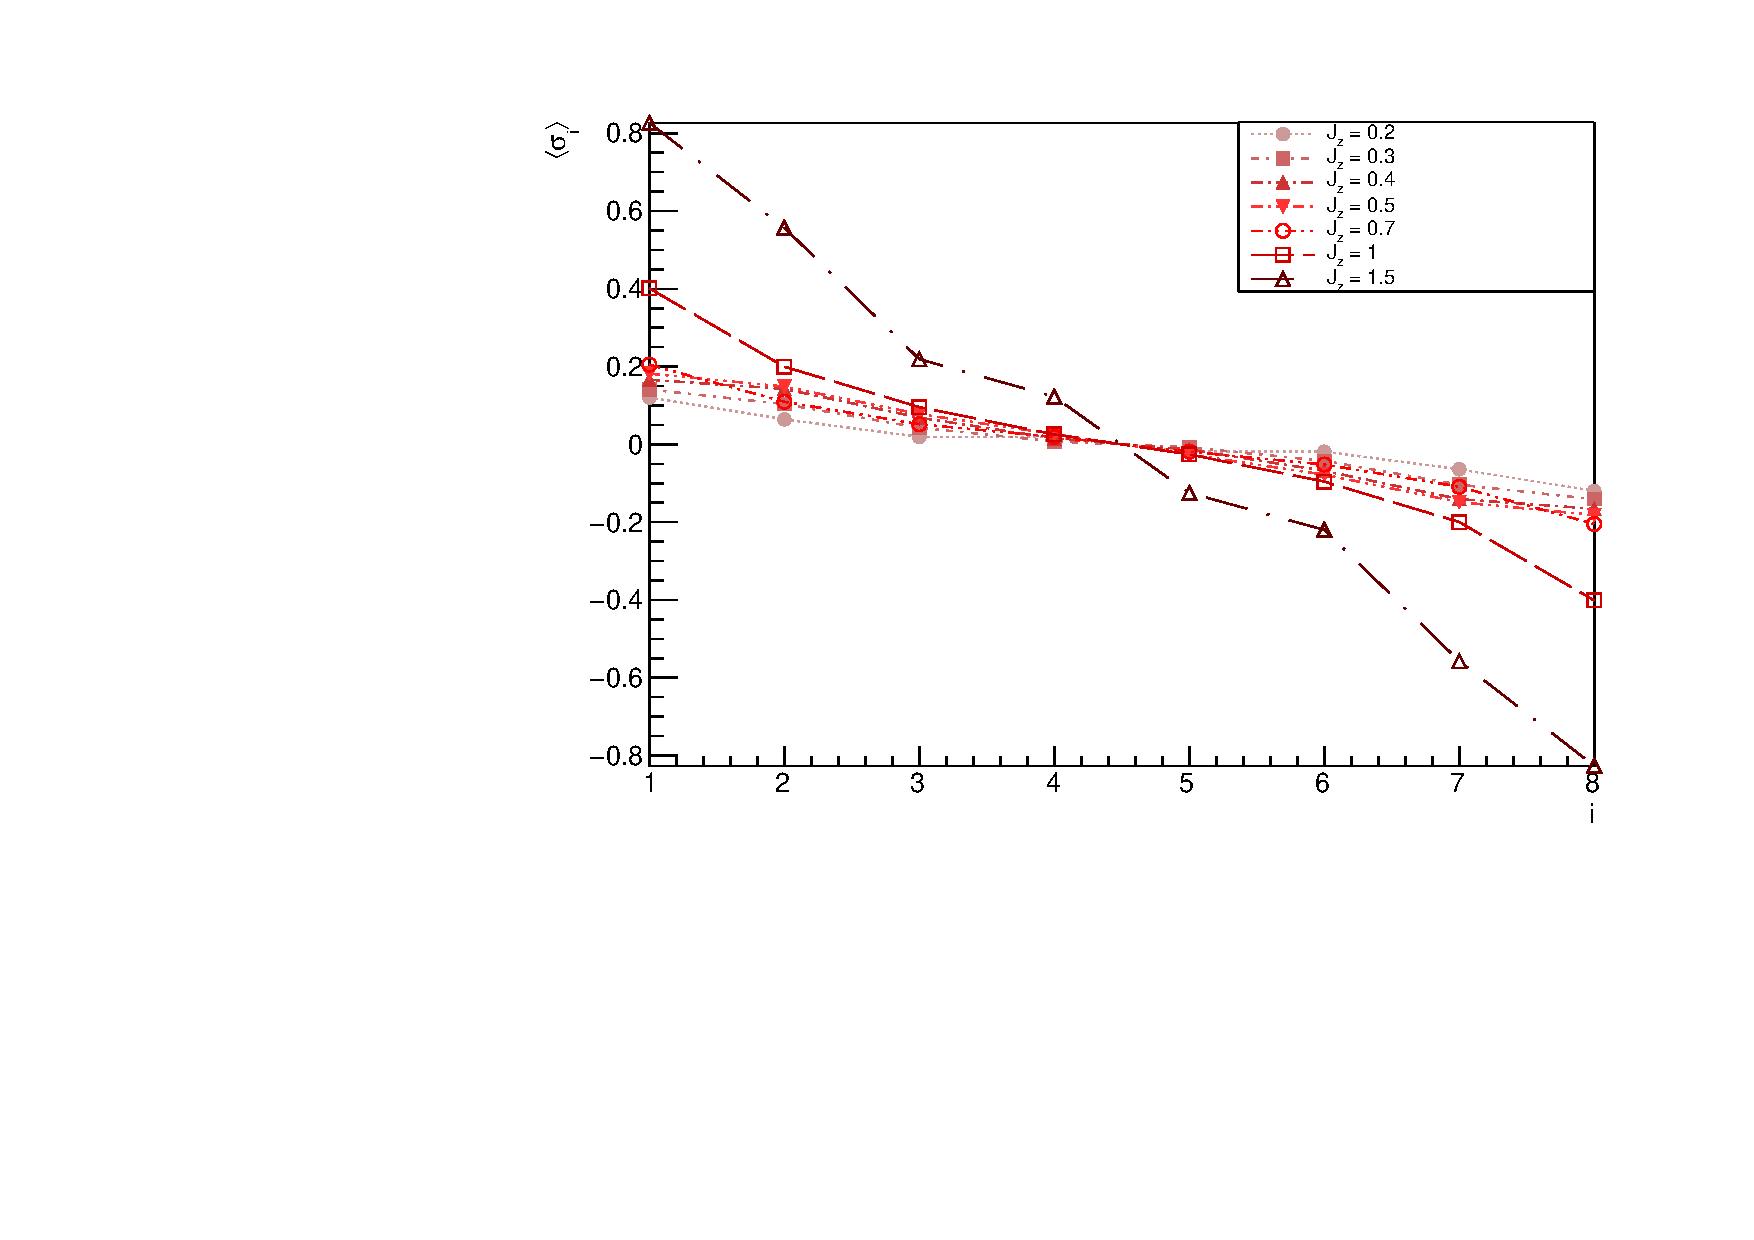
\includegraphics[scale=0.7]{Figures/8sites_LMvsJz.pdf}
    %\caption{Magnetization profile of a 8-sites chain, with $\gamma = 1$ for %several values of $J_z$. Data obtained from MPO method.}
    %\label{fig:8sites_LMvsJz}
%\end{figure}

%\begin{figure}[H]
    %\centering
    %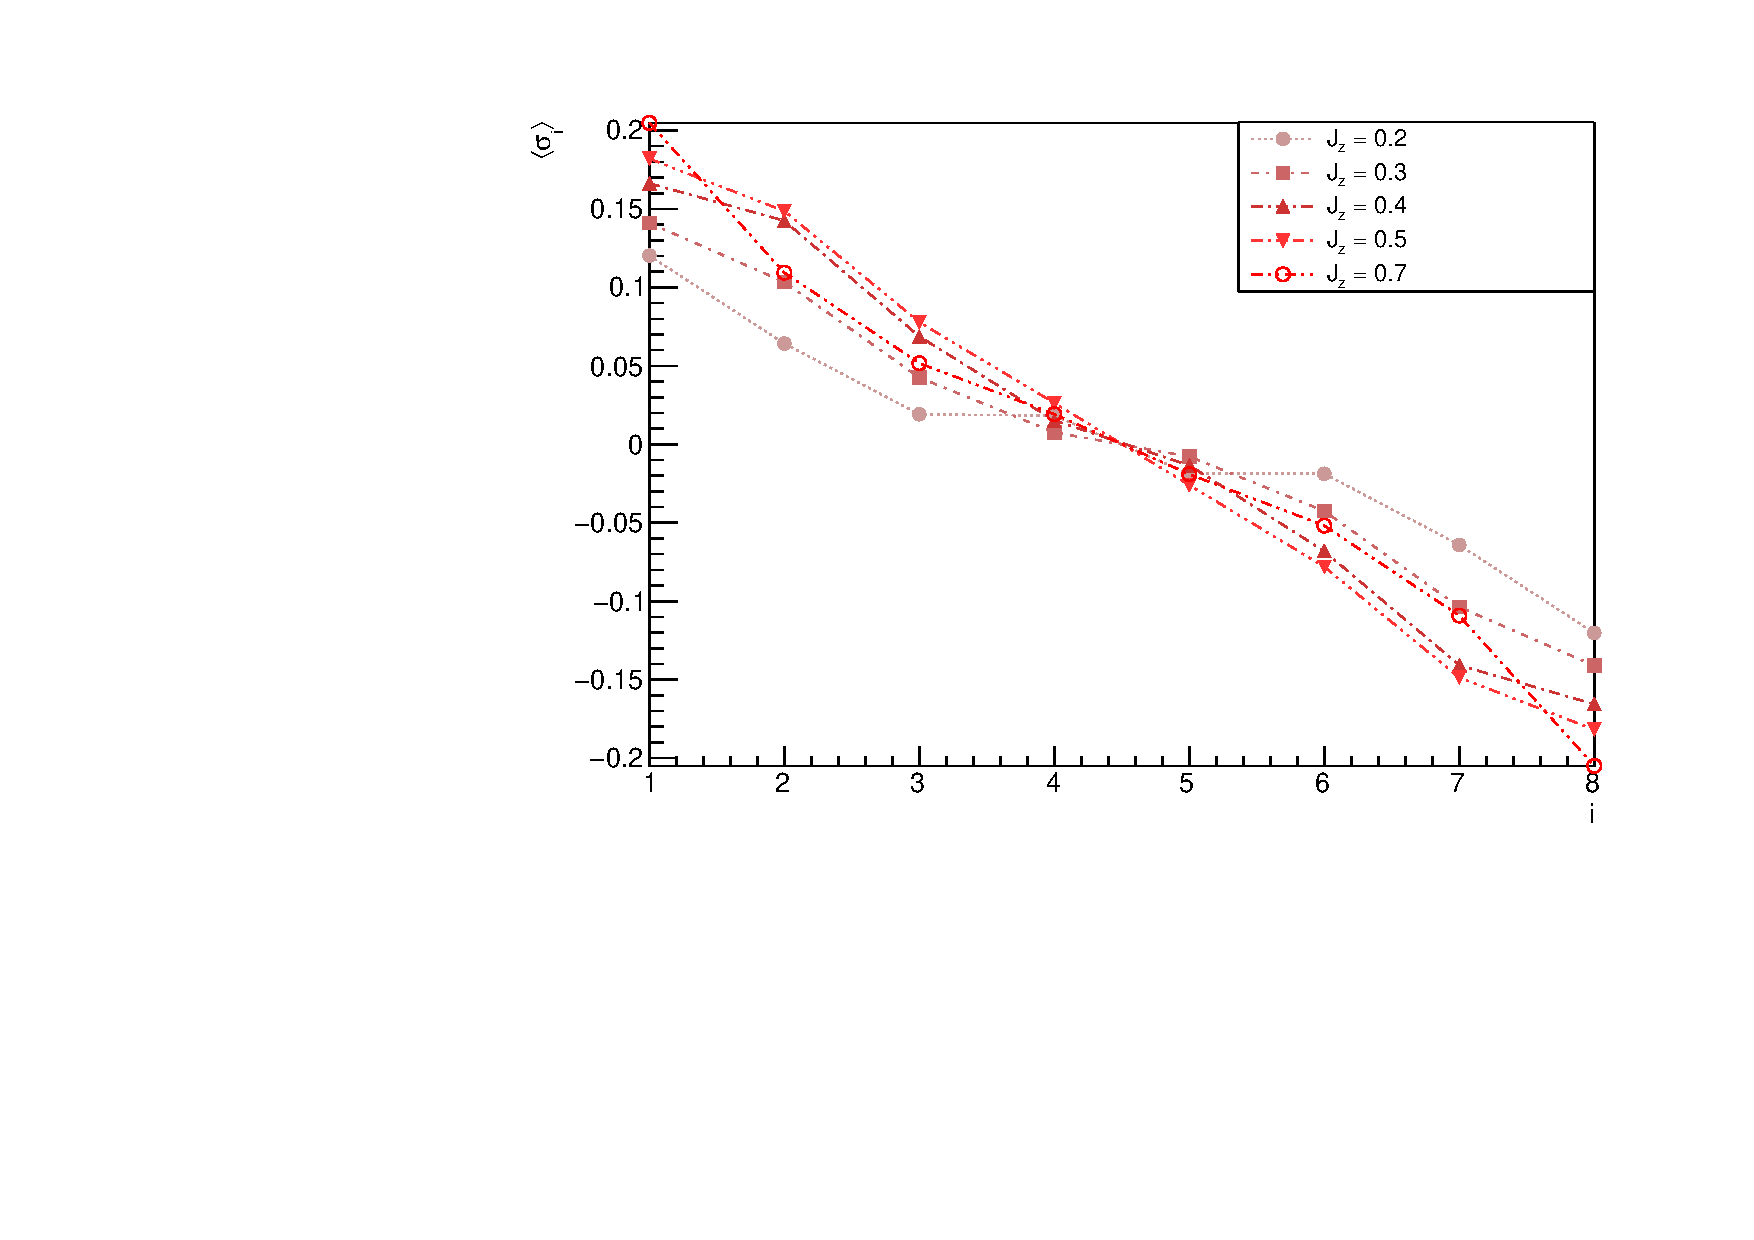
\includegraphics[scale=0.7]{Figures/8sites_LMvsLowJz.pdf}
    %\caption{Magnetization profile of a 8-sites chain, with $\gamma = 1$ for $J_z %\leq 0.7$. Data obtained from MPO method.}
    %\label{fig:8sites_LMvsLowJz}
%\end{figure}

%\begin{figure}[H]
    %\centering
    %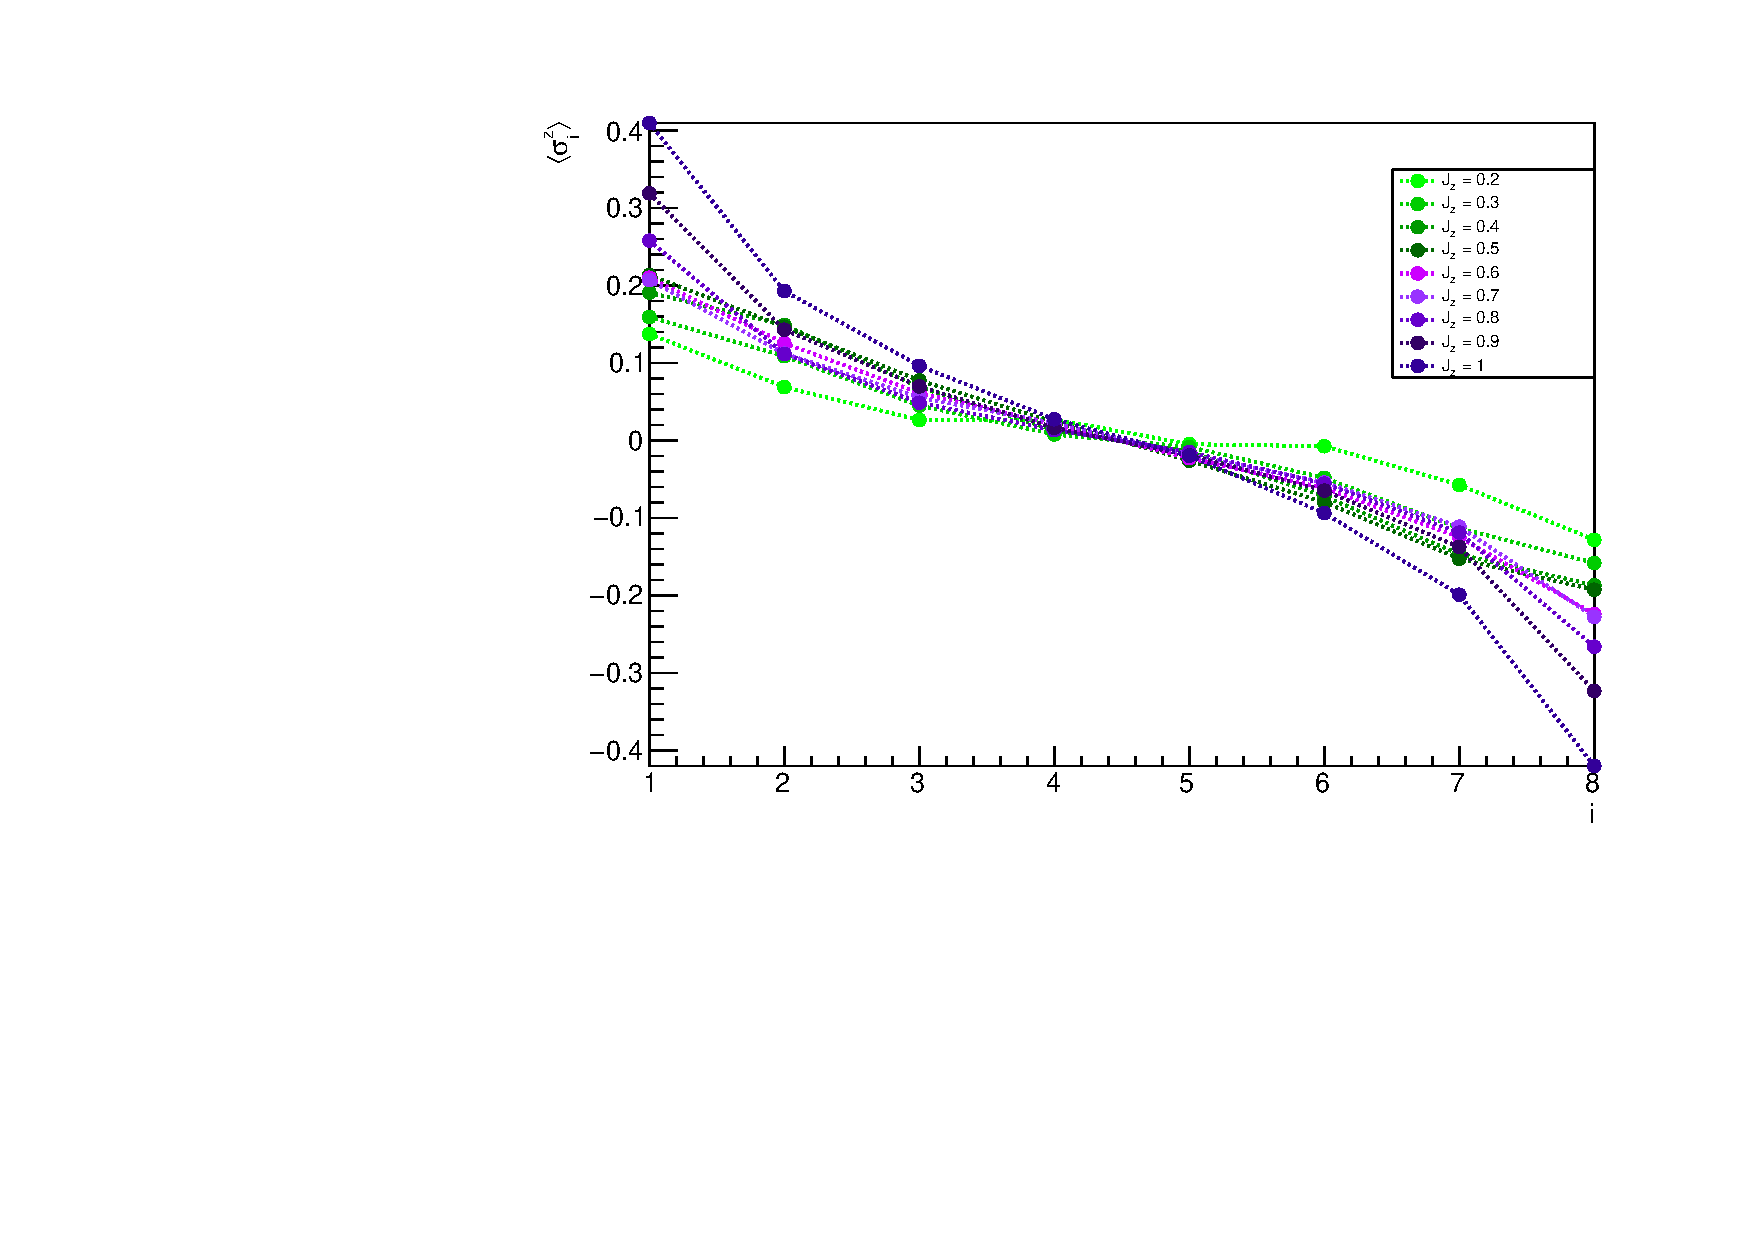
\includegraphics[scale=0.7]{Figures/8sites/8sites_LMvsJzQT.pdf}
    %\caption{Magnetization profile of a 8-sites chain, with $\gamma = 1$ for %several values of $J_z$. Data obtained from QT method.}
    %\label{fig:8sites_LMvsJzQT}
%\end{figure}

%\begin{figure}[H]
    %\centering
    %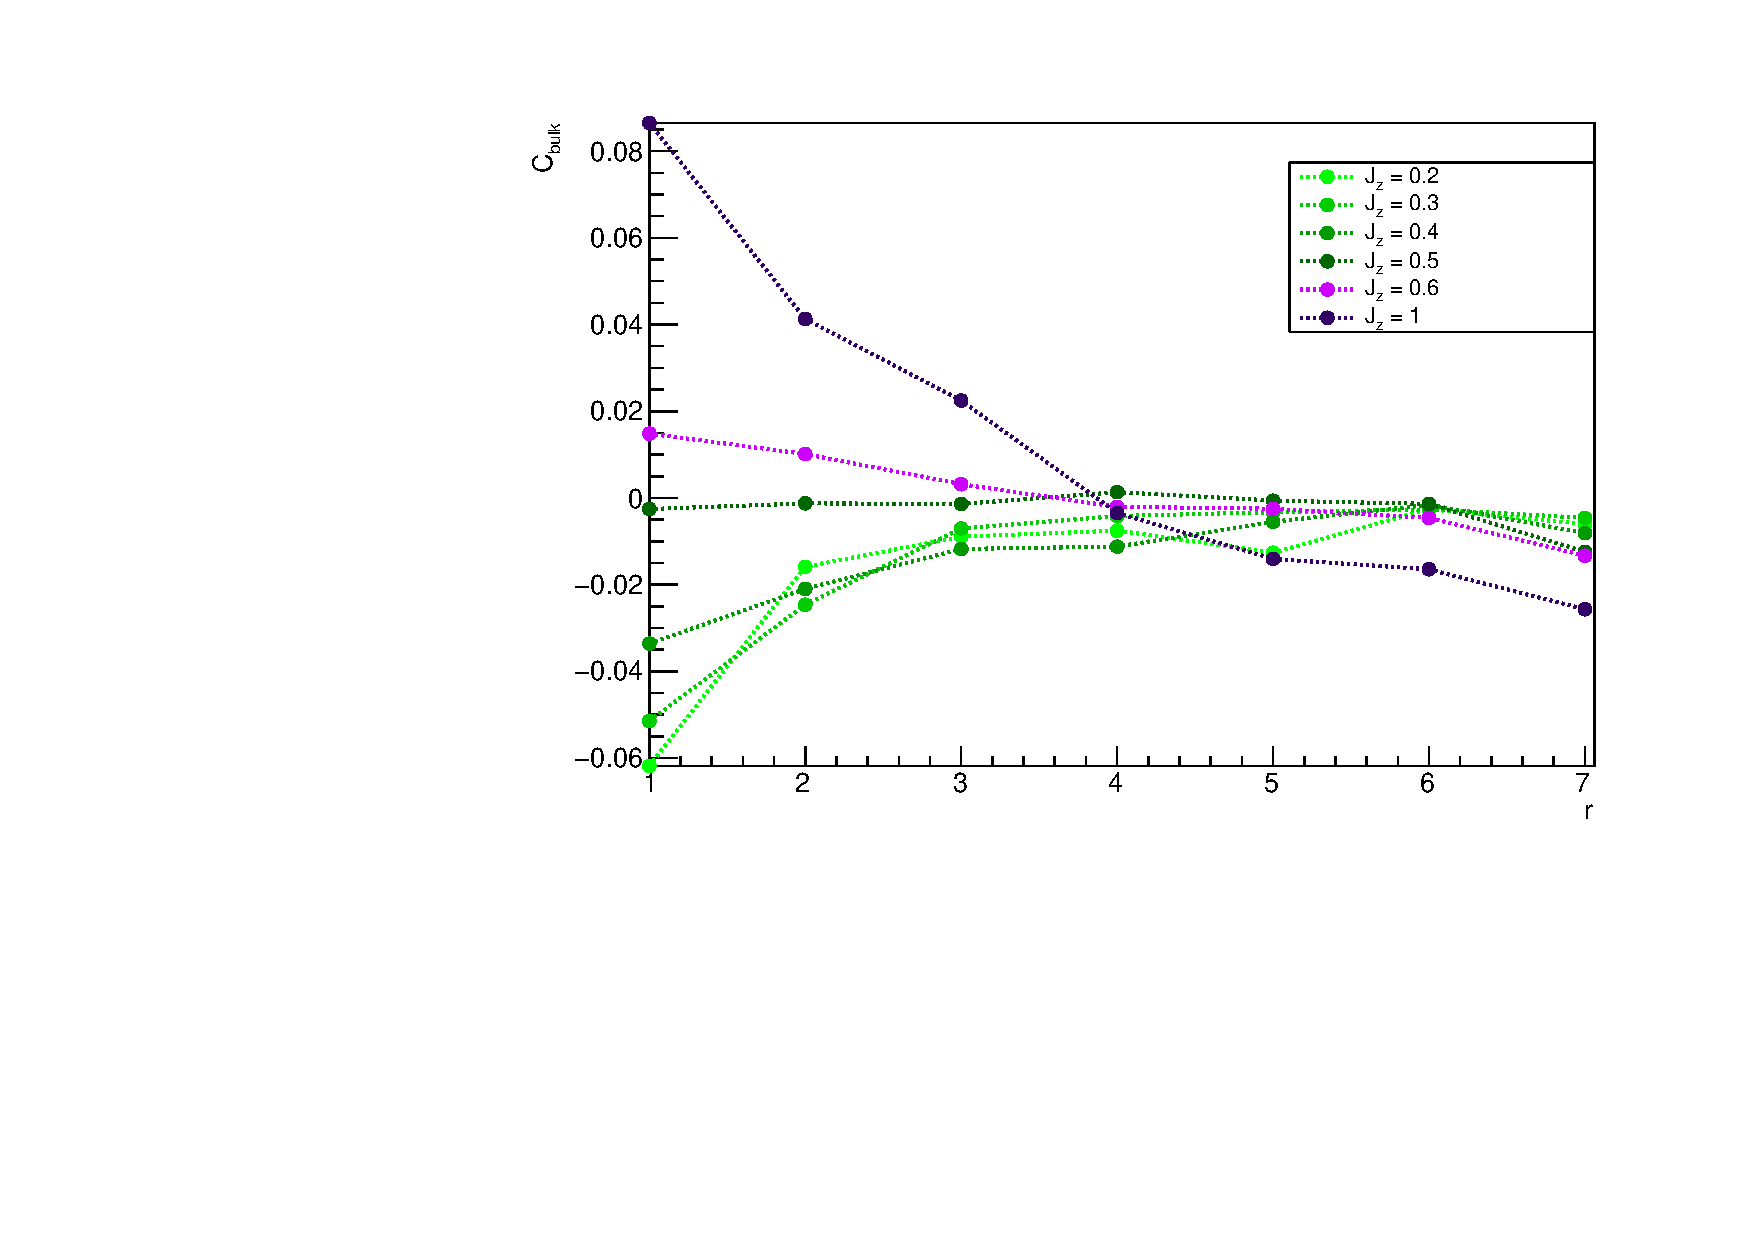
\includegraphics[scale=0.7]{Figures/8sites/8sites_CFBulkvsLowJz_QT.pdf}
    %\caption{Bulk correlation function of a 8-sites chain, with $\gamma = 1$ for %several values of $J_z \leq 1$. Data obtained from QT method.}
    %\label{fig:8sites_CFBulkvsLowJz_QT}
%\end{figure}


%\begin{figure}[H]
    %\centering
    %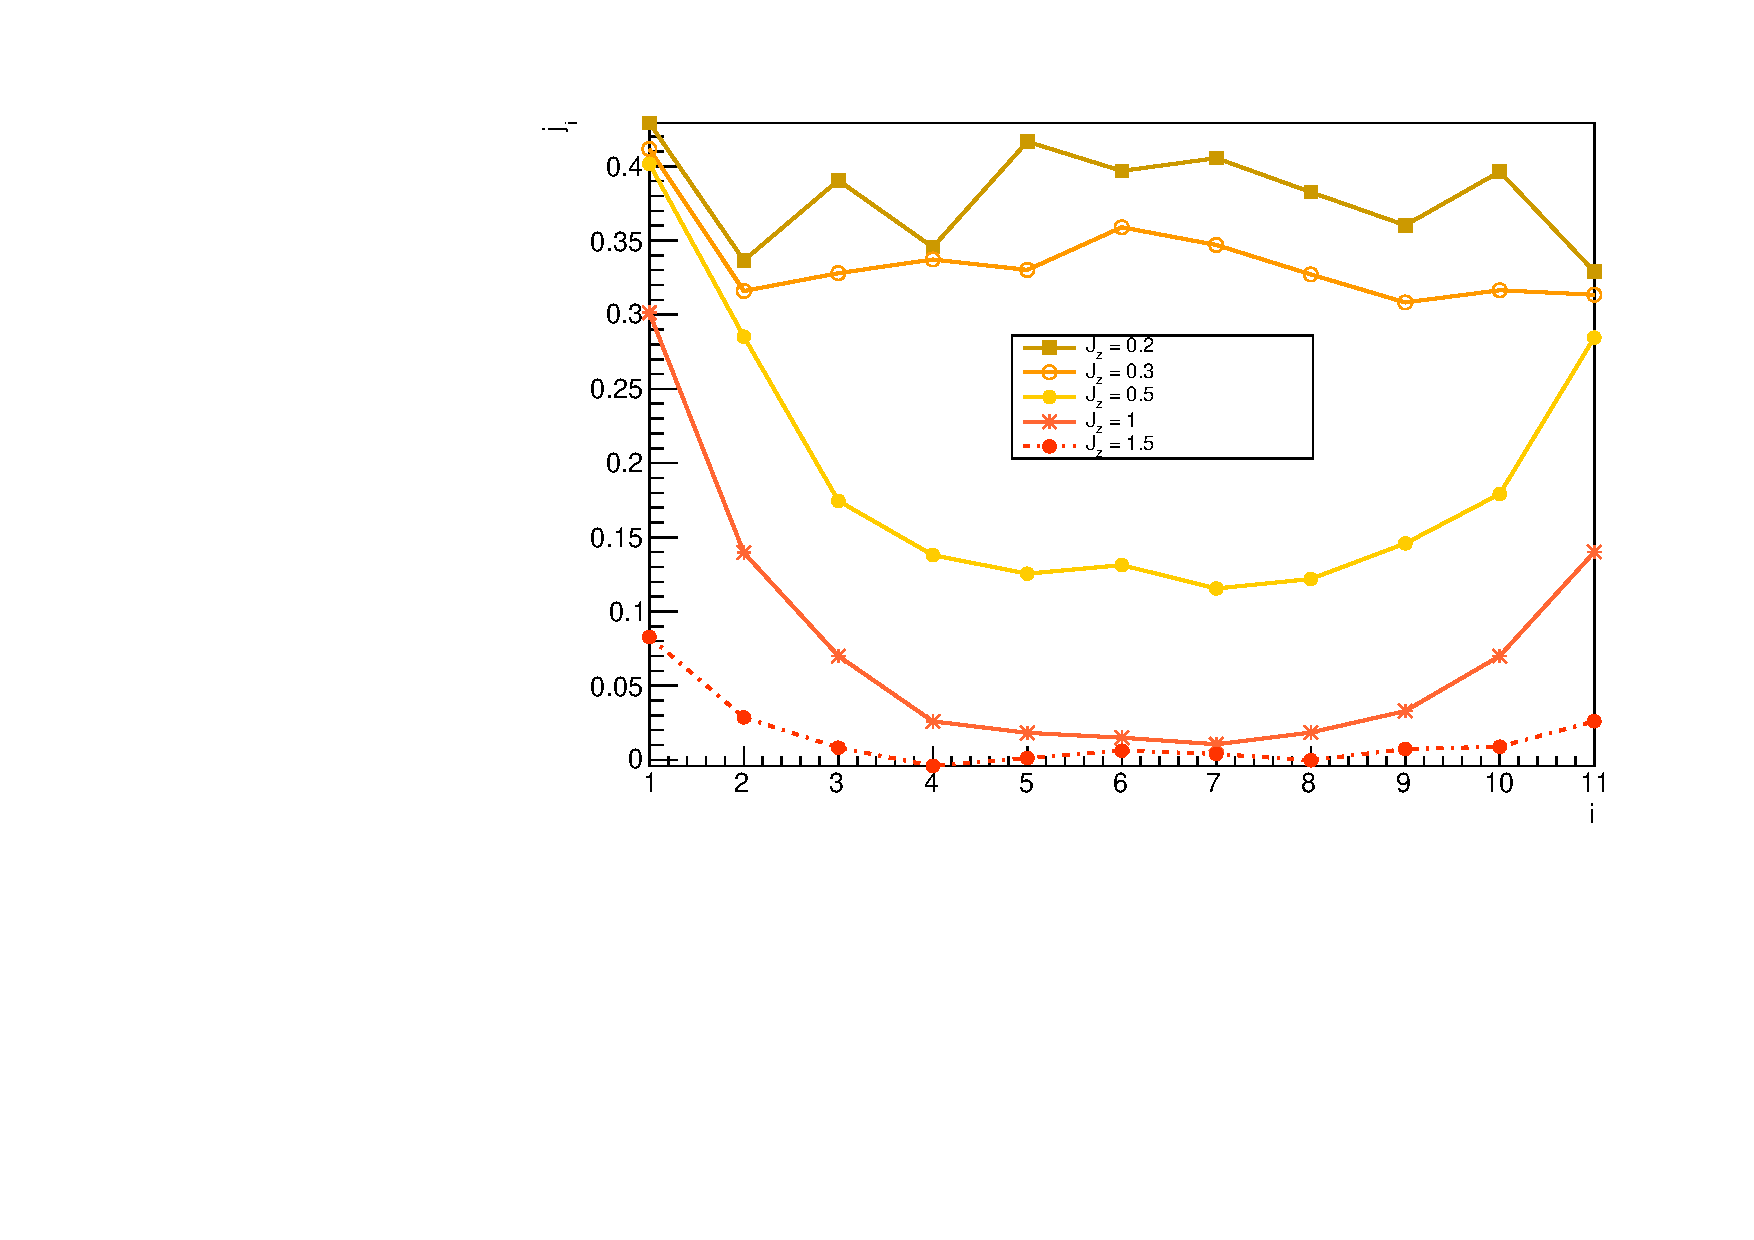
\includegraphics[scale=0.7]{Figures/12sites_spinCurrVSJz.pdf}
    %\caption{Spin current of a 12-sites chain, with $\gamma = 1$ for several values %of $J_z$. Data obtained from MPO method.}
    %\label{fig:12sites_spinCurrVSJz}
%\end{figure}

%\begin{figure}[H]
    %\centering
    %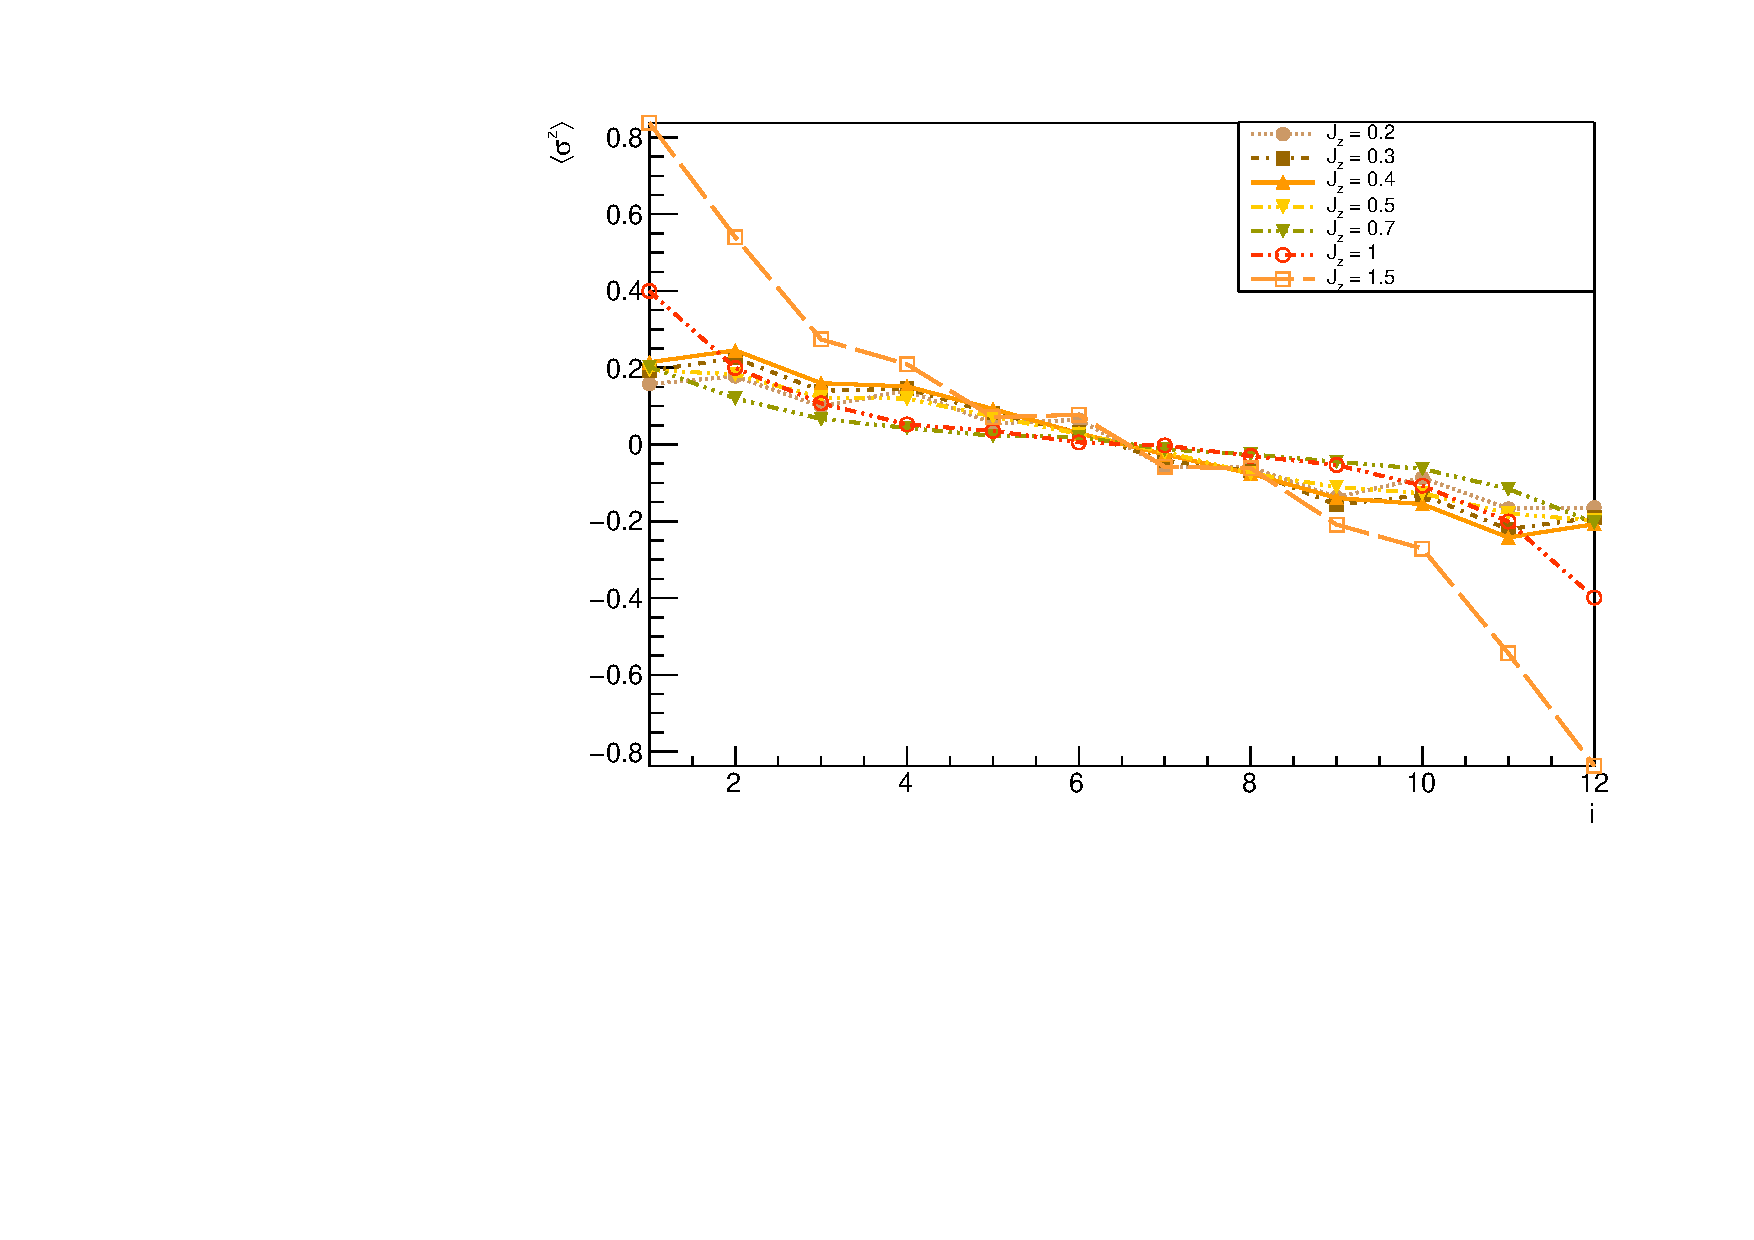
\includegraphics[scale=0.7]{Figures/12sites/12sites_LMvsJz.pdf}
    %\caption{Magnetization profile of a 12-sites chain, with $\gamma = 1$ for $J_z %\leq 0.7$. Data obtained from MPO method.}
    %\label{fig:my_label}
%\end{figure}

%\begin{figure}[H]
    %\centering
    %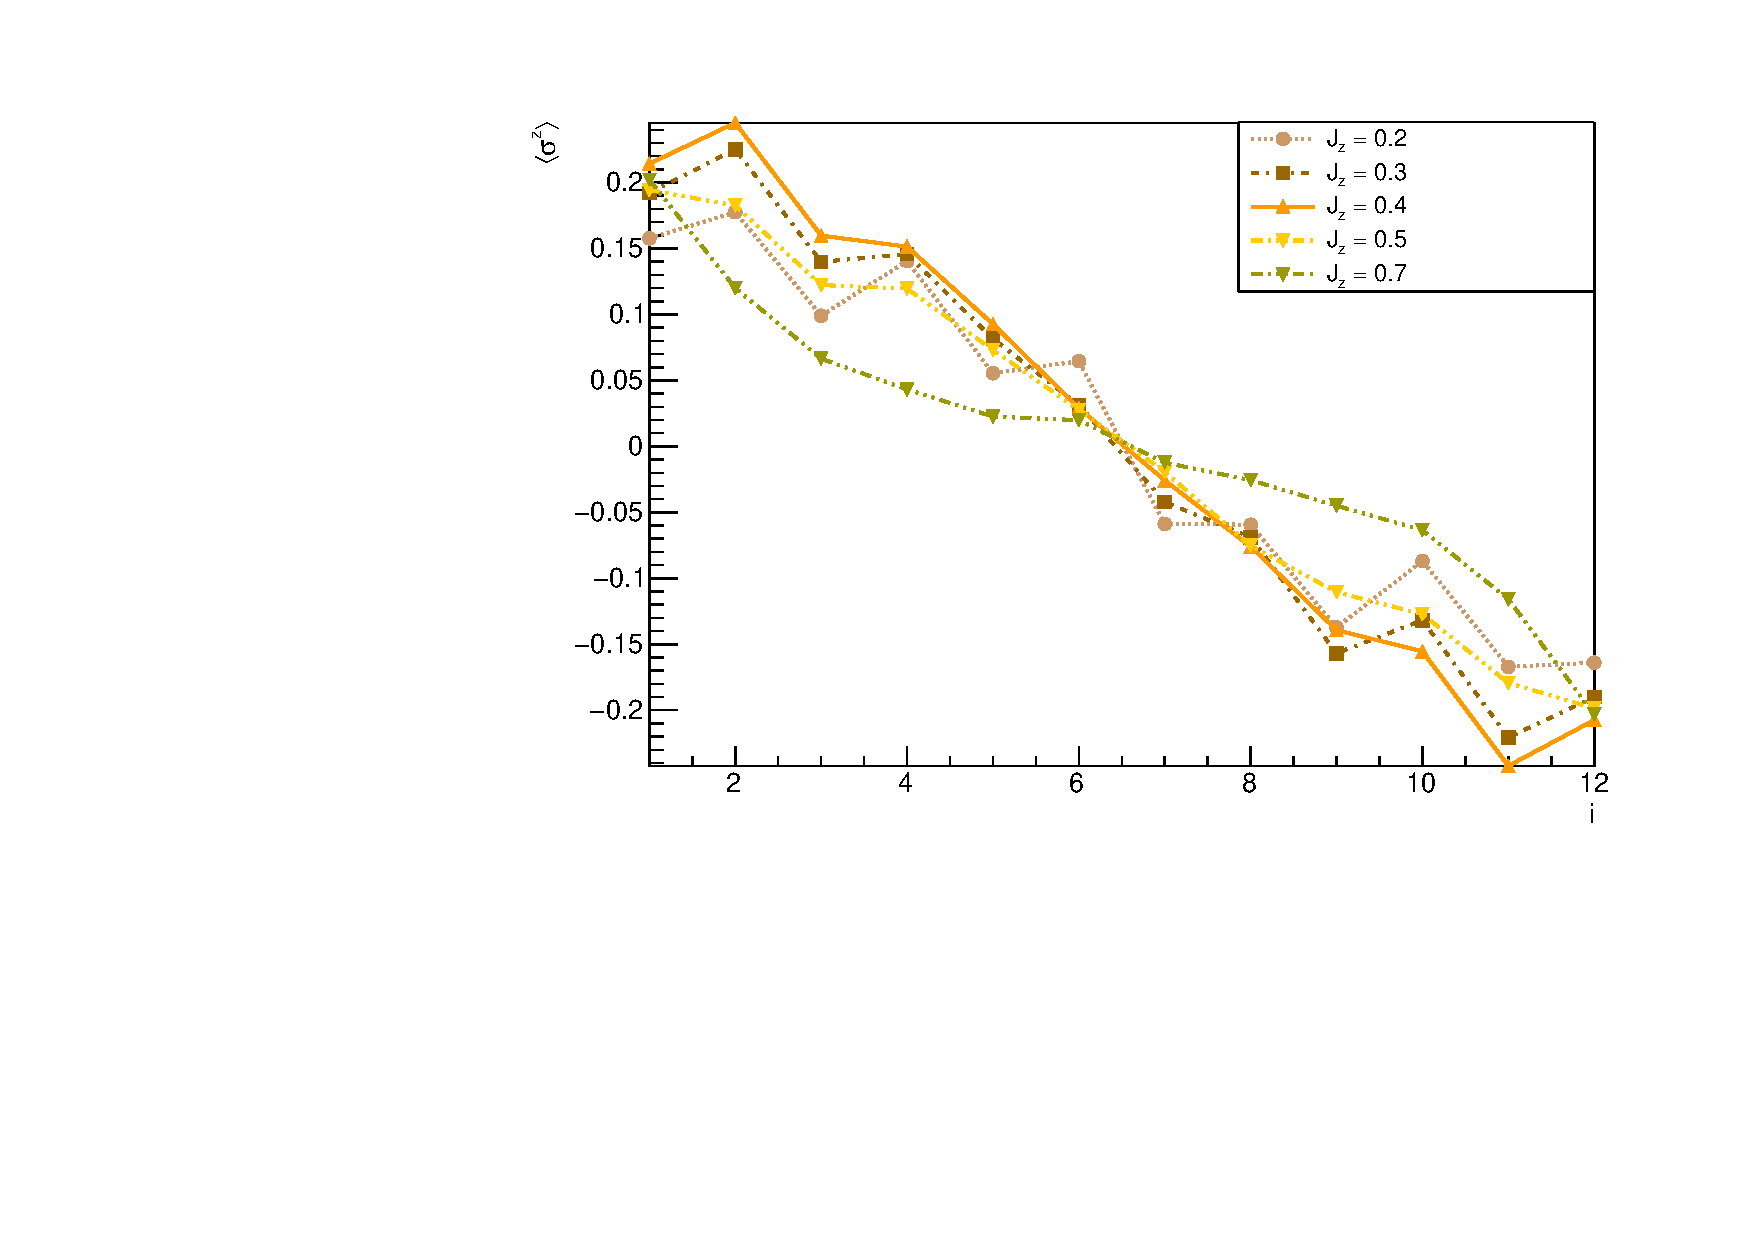
\includegraphics[scale=0.7]{Figures/12sites/12sites_LMvsLOWJz.pdf}
    %\caption{Magnetization profile of a 12-sites chain, with $\gamma = 1$ for $J_z %\leq 0.7$. Data obtained from MPO method.}
    %\label{fig:my_label}
%\end{figure}

%\begin{figure}[H]
    %\centering
    %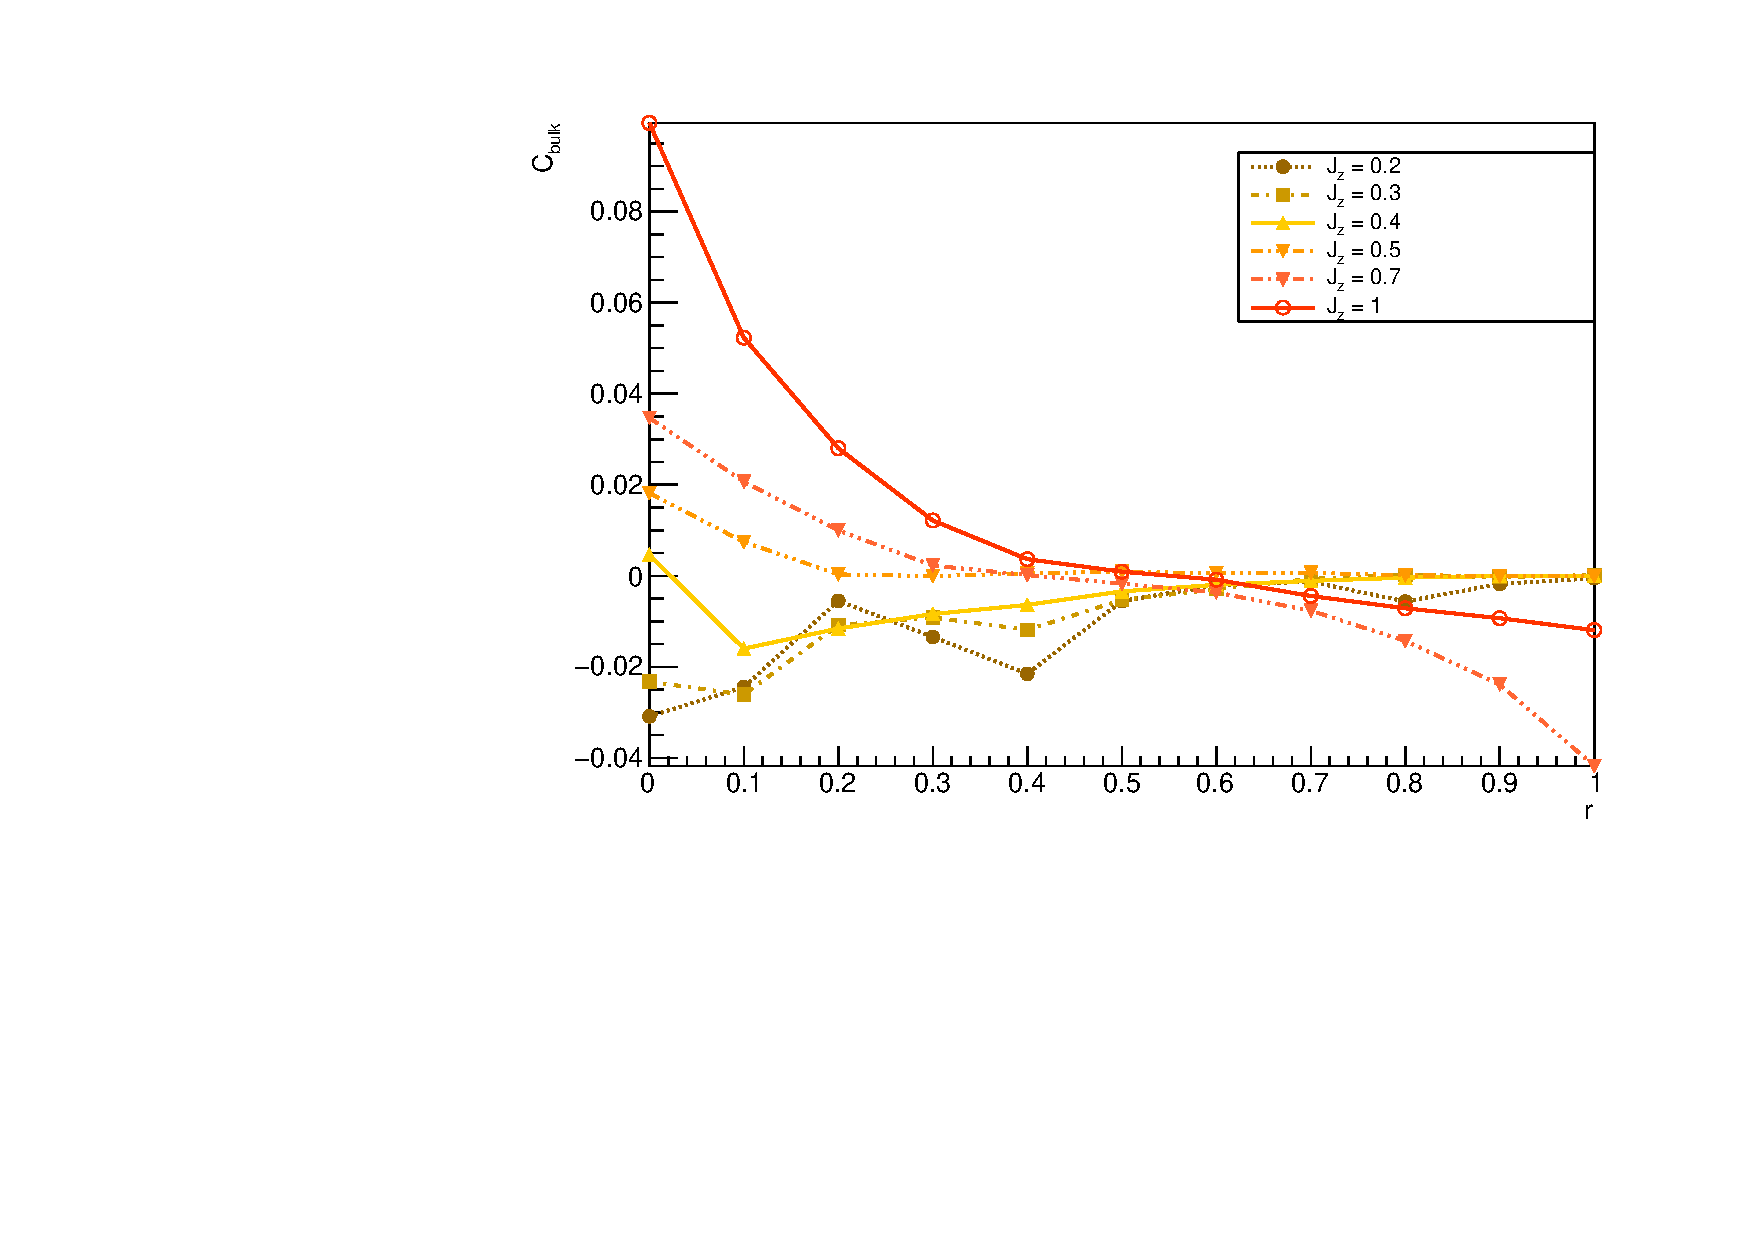
\includegraphics[scale=0.7]{Figures/12sites/12sites_CFBulkVSLowJz.pdf}
    %\caption{Bulk correlation function of a 12-sites chain, with $\gamma = 1$ for %several values of $J_z \leq 1$. Data obtained from MPO method.}
    %\label{fig:12sites_CFBulkVSLowJz}
%\end{figure}

\begin{figure}[H]
    \centering
    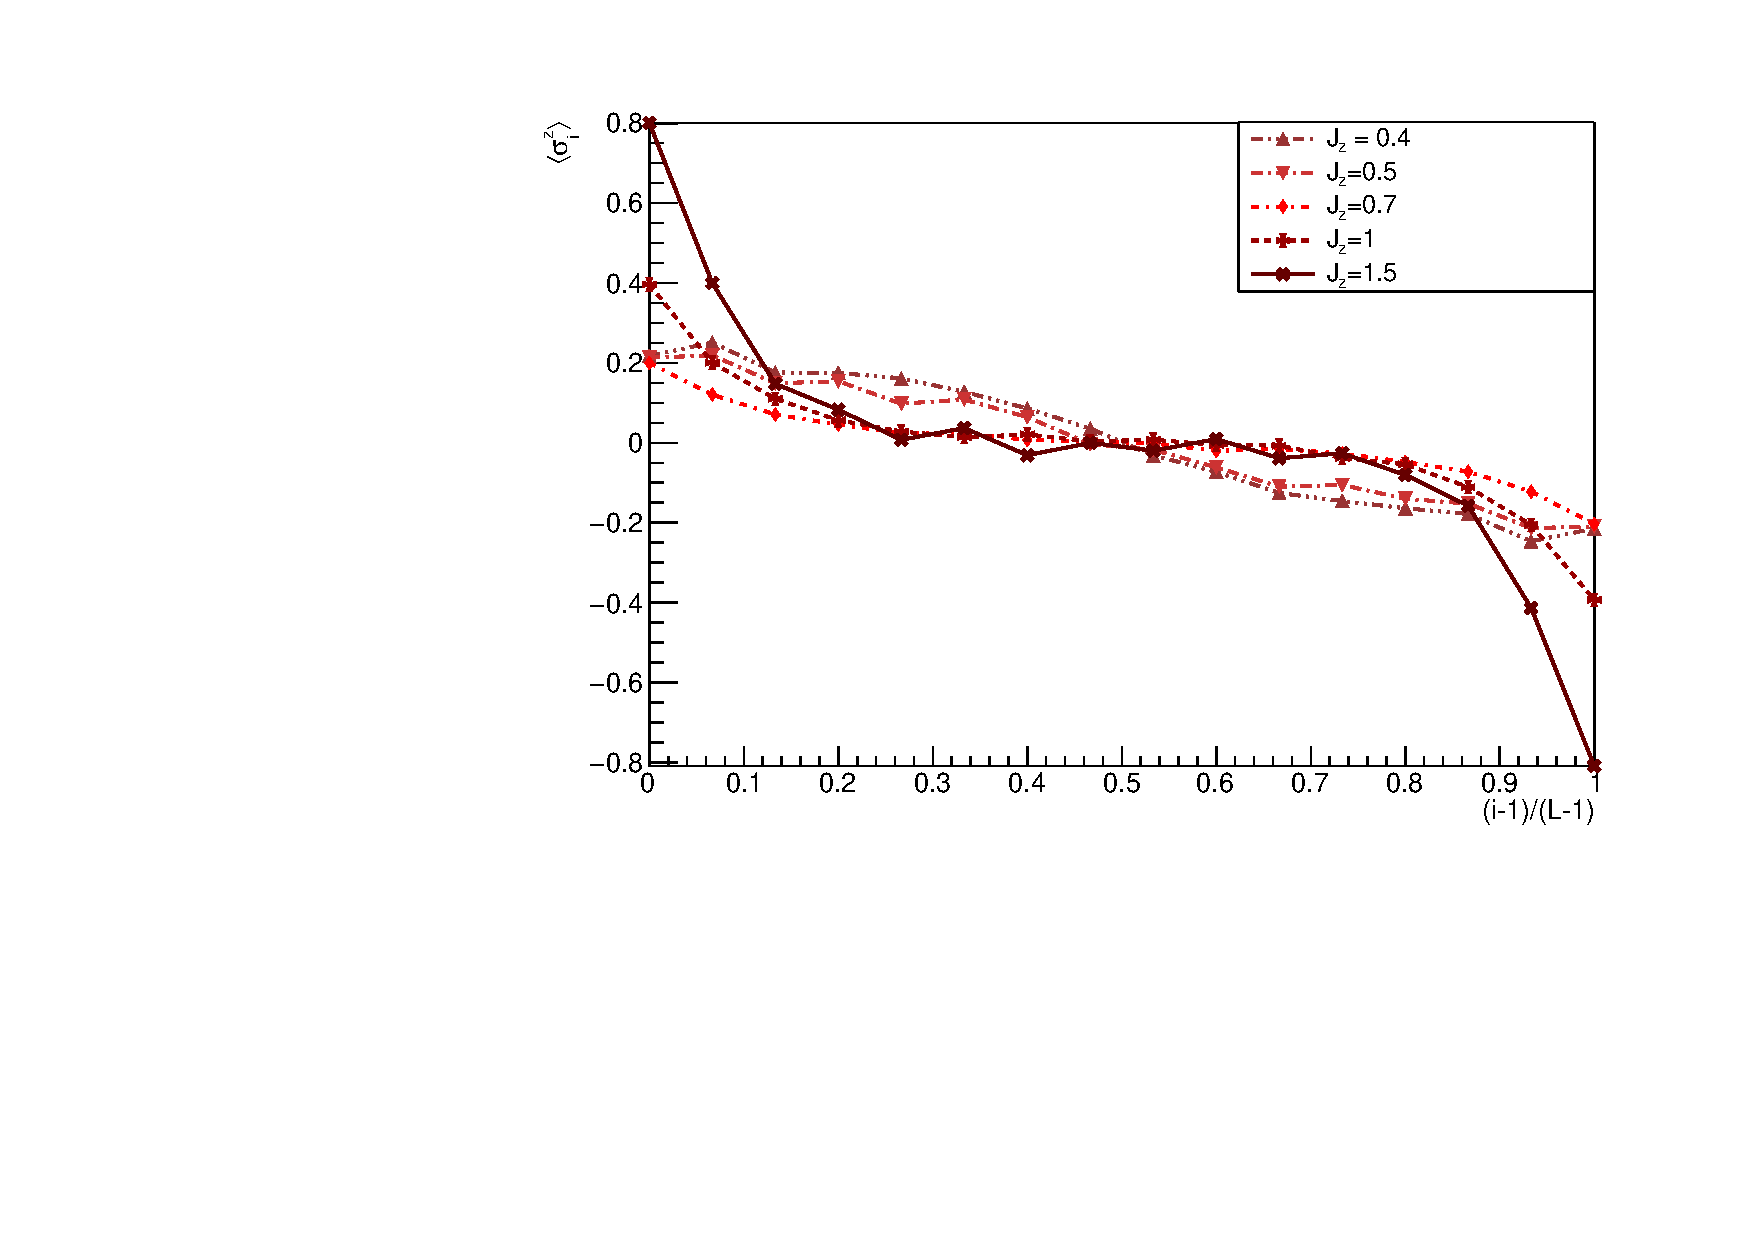
\includegraphics[scale=0.7]{Figures/16sites/16sites_LMvsJz.pdf}
    \captionsetup{width=1.\linewidth}
    \caption{Magnetization profile of a 16-sites chain, with $\gamma = 1$ for several values of $J_z$. Data obtained from MPO method.}
    \label{fig:16sites_LMvsJz}
\end{figure}

The magnetization profile (displayed in fig.~\ref{fig:16sites_LMvsJz}) for $J_z \geq 1$ shows a similar behaviour to the one seen in the previous chapter, when we considered variation of $\gamma$: the variation of the coupling constant $J_z$ has a similar effect of the one caused by the variation of the dissipation rate $\gamma$. 

For small values of $J_z$, i.e. $J_z < 1$, a couple of things can be noted. First of all, for all the $J_z < 1$ the $\langle \sigma^z \rangle$ of the first and of the last spin of the chain is constant. This can be explained as an unimportance of the Hamiltonian terms in relation to dissipation. 

It is worth noting that in the magnetization profile does not arise the discontinuity noticed in the trend of the spin current, for $J_z < 0.5$. Analyzing the two-point correlation function can be helpful in order to brighten this hypothesis.

%\begin{figure}[H]
    %\centering
    %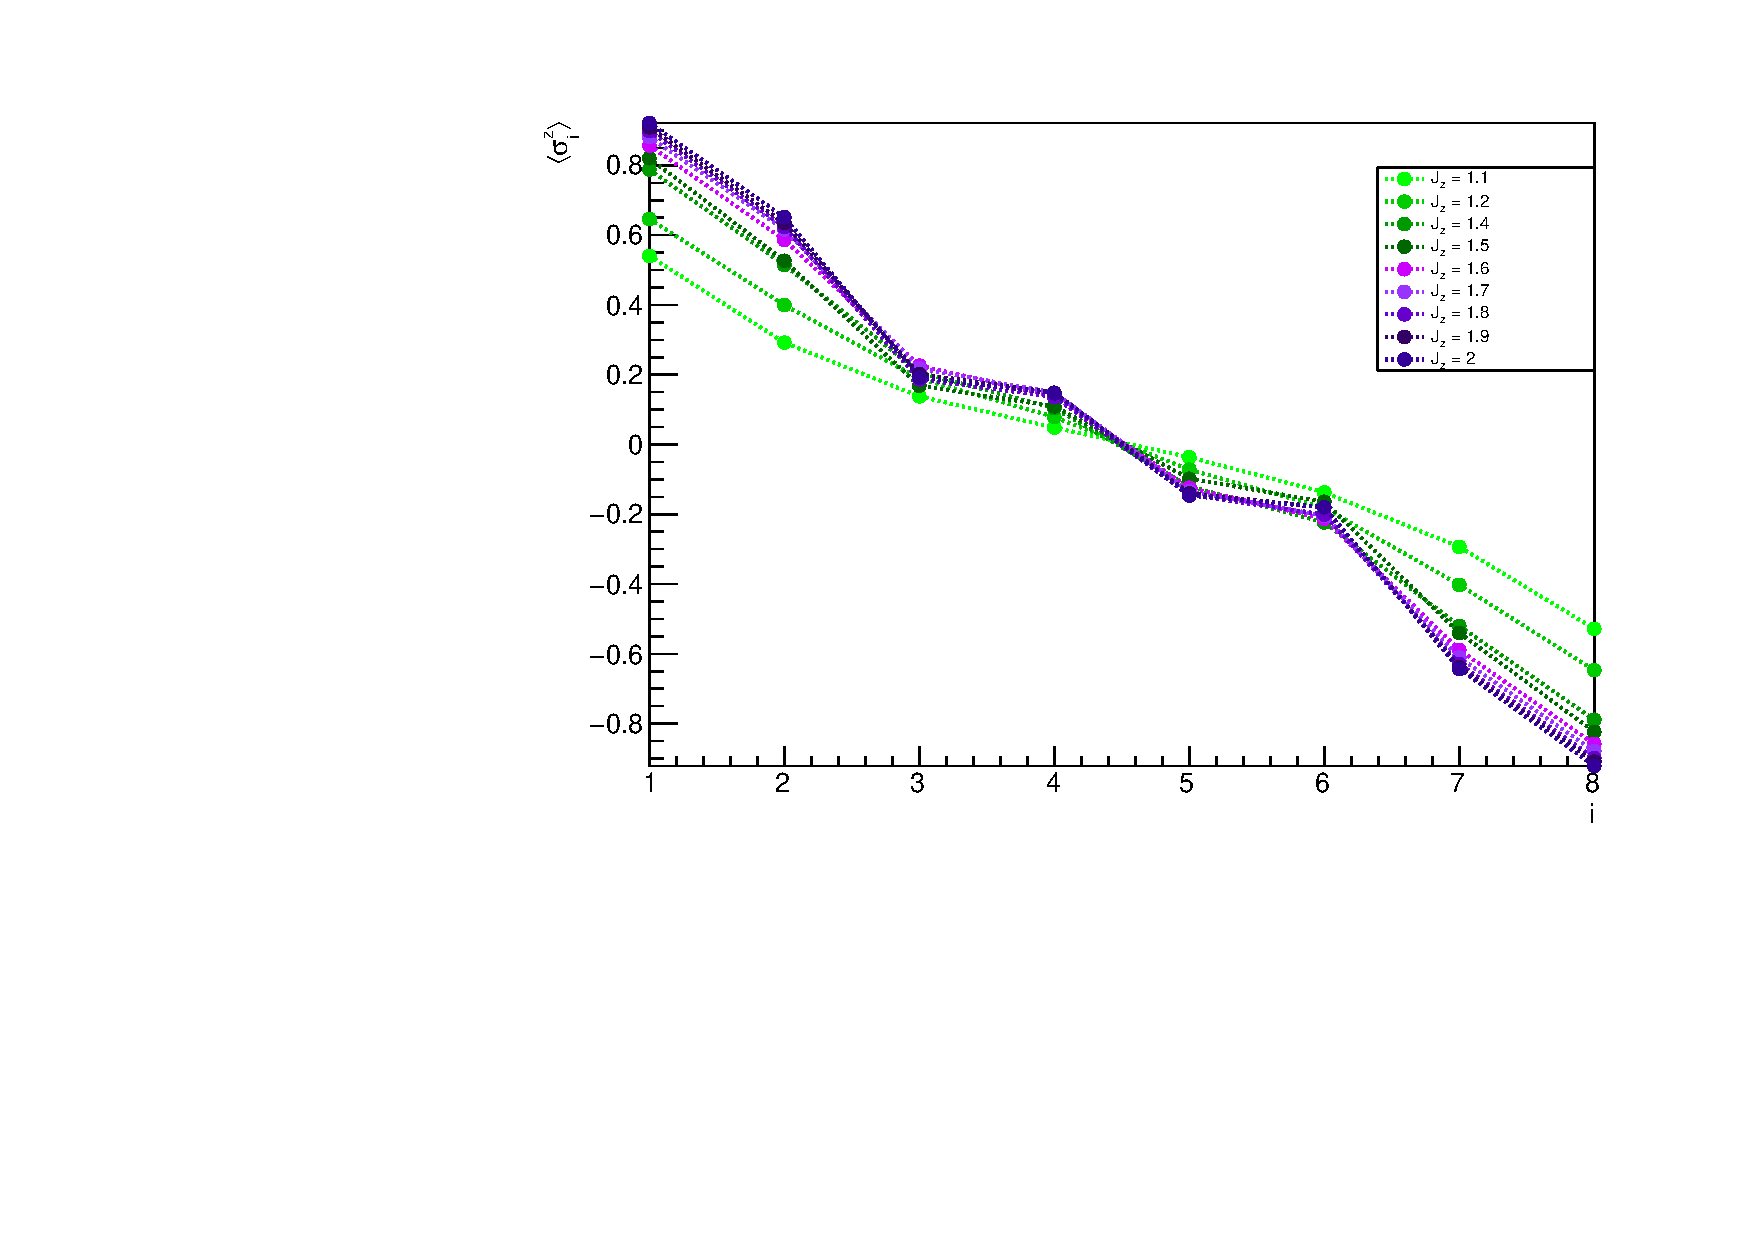
\includegraphics[scale=0.7]{Figures/8sites/8sites_LMvsJz_gtOneQT.pdf}
    %\caption{Magnetization profile of a 8-sites chain, with $\gamma = 1$ for %several values of $J_z \geq 1.1$. Data obtained from QT method.}
    %\label{fig:8sites_LMvsJz_gtOneQT}
%\end{figure}



\begin{figure}[H]
    \centering
    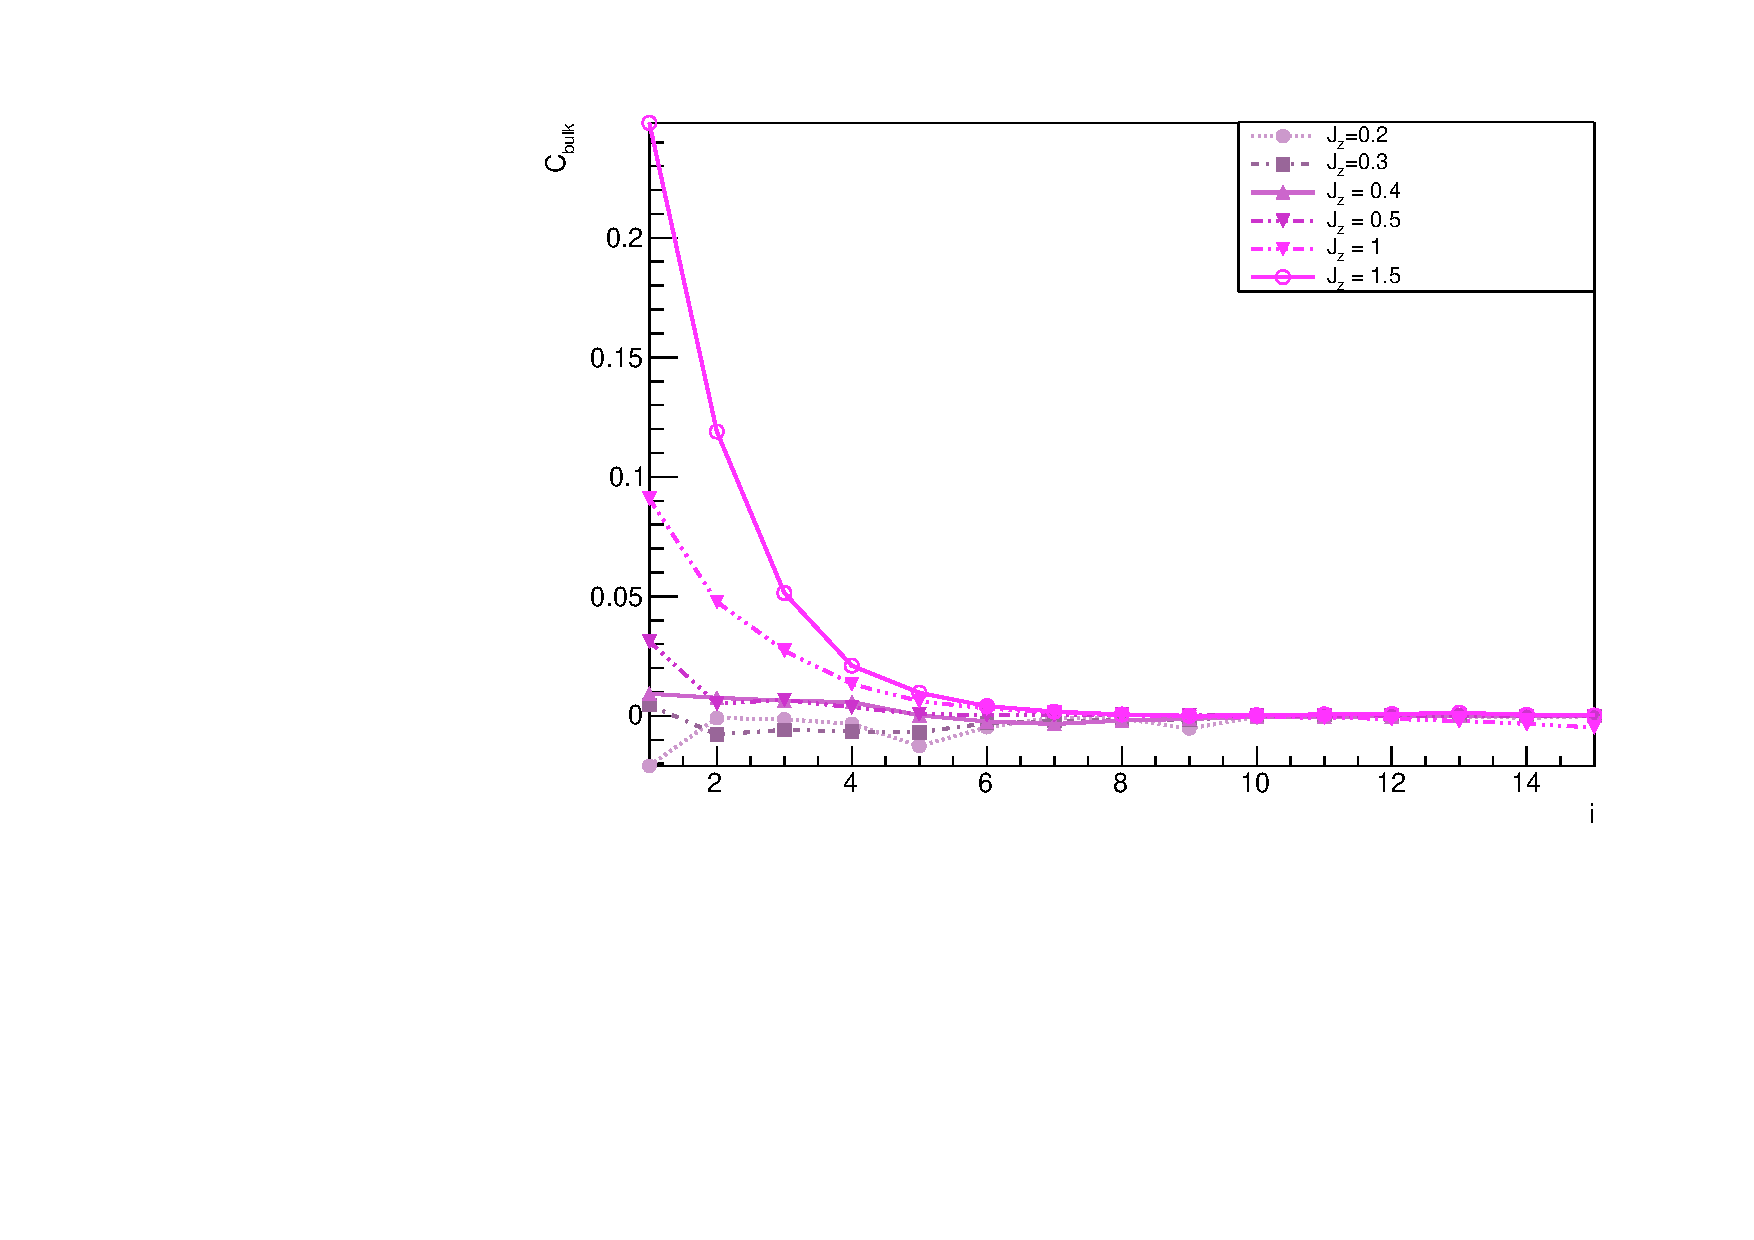
\includegraphics[scale=0.7]{Figures/16sites/16sites_CFBulkCONNvsJz.pdf}
    \captionsetup{width=1.\linewidth}
    \caption{Correlation function of a 16-sites chain, with $\gamma = 1$ for several values of $J_z$. Data obtained from MPO method.}
    \label{fig:16sites_CFBulkCONNvsJz}
\end{figure}

The two-point correlation function, displayed in fig.~\ref{fig:16sites_CFBulkCONNvsJz}, for $J_z \geq 0.5$ shows a behaviour similar to that seen in the previous chapter, with an exponential profile of the correlation function. In this case, however, there is a discontinuity in its behaviour for $J_z < 0.5$. Indeed, the plots show a null correlation function for such values of $J_z$, trend that is consistent with the profile of spin current in fig.~\ref{fig:16sites_SpinCurrVaryingJz}.

%%%%%%%%%%%%%%%%%%%%%%%%%%%%%%%%%%%%%%%%%%%%%%%%%%%%%%%%%%%%%%%%%%
%%%%%%%%%%%%%%%%%%%%%%%%%%%%%%%%%%%%%%%%%%%%%%%%%%%%%%%%%%%%%%%%%%
%%%%%%%%%%%%%%%%%%%%%%%%%%%%%%%%%%%%%%%%%%%%%%%%%%%%%%%%%%%%%%%%%%
